\documentclass[oneside, 12pt]{extbook}

% imports + page geometry
\usepackage{geometry}
\usepackage{graphicx}
\usepackage{listings}
\usepackage[dvipsnames]{xcolor}
\usepackage[italian]{babel}
\usepackage{amsmath}
\usepackage{mathrsfs}	% for pretty symbols
\usepackage{mathtools}
\usepackage{amssymb}
\usepackage[utf8]{inputenc}

\DeclarePairedDelimiter{\abs}{\lvert}{\rvert}

\geometry{
        a4paper, 
        top = 2cm,
        left = 1.5cm,
        right = 1.5cm,
        bottom=2cm
}

\title{Hardware, Electromagnetic and Localization Security}
\author{Pierciro Caliandro}



\begin{document}
\maketitle
\chapter{Introduzione}
\section{Introduzione}
Attacco fisico invece di informatico, viene applicato un attacco di tipo EM: si mandano segnali fisici su un apparato per indurre malfunzionamento o rubare dati.\\Si arriva all'impatto sull'elettronica, si cerca quindi di ottenere dei rudimenti di sicurezza fisica: 3 aspetti di livello diverso, dal sistema, alla parte di comunicazione alla parte elettronica.\\Aspetti fondamentali:\\
- short range vulnerabilities: dispositivi medici avranno tutte funzionalità wireless: pacemakers va configurato, quindi in base alla risposta configura il dispositivo con un accoppiamento di tipo NFC, in futuro anche le protesi più "sciocche" come una placca per le ossa saranno wireless, sarà funzionalizzato con diversi sensori per verificare infezioni etc... ed essere letto da fuori.\\Qualunque oggetto impiantato sarà funzionalizzato, a seguito di interventi di qualunque tipo (punti di sutura etc...) che sarà provvisto di sensori.\\È tutto vittima di attacco informatico, per rubare dati in maniera non intenzionale.\\Il corpo diventa quindi un nodo di Internet, si parla di \textbf{Internet of the bodies}, ci possono essere diversi tipi di sensori che interagiscono.C'è una lista svariata di oggetti di medica che controllano le attività fisiche.\\L'accesso non intenzionale al dispositivo ha un impatto potenzilamente dirompente, lo scenario va a parare in una medicina guidata dai dati dove si mischiano diverse discipline, è il concetto di \textbf{medicina di precisione}: parte dalle terapie oncologiche, in ingegneria è la capacità della medicina di apprendere. Se la terapia oggi va bene, il corpo umano cambia e quindi tale terapia può necessitare di essere aggiornata.\\Il punto critico è che per rendere questa visione operabile, occorre avere sistemi pervasivi + AI per poter poi tirare fuori una cura.\\È una medicina assistiva che può essere integrata con sensori nella casa che controllano l'utente paziente, si parla di 3 tipi di dispositivi, ci interessa capire come questi comunicano e non il loro funzionamento:
\begin{itemize}
    \item wearable
    \item epidermici
    \item implantable
\end{itemize}
che devono avere la safety by design, quindi non devono fare male quando indossati, la security by design e quindi essere sicuri da progettazione e poi la privacy by design, quindi capire come è possibile che i dati vengano usati impropriamente.\\Abbiamo ad esempio strumenti epidermici che rilascia cortisolo quando ad esempio viene misurato da un sensore che scende sotto soglia una certa misura.\\Ci sono quindi 3 tipi di links:
\begin{itemize}
    \item on-body link
    \item through-the-body
    \item off-the-body
\end{itemize}
Analizzeremo tutto a livello di modello fisico-matematico.\\Ci sono poi problemi per quanto riguarda la lettura dei dati, qui c'è la corrispondenza fisica di come si leggono tali dati, ma c'è anche il come si fa per accedere al dispositivo, ad esempio ci sono delle micro-antenne non volute.
\subsection{Introduzione generale sulla cybersecurity}
Si completa il concetto di cybersecurity con gli aspetti fisici e di comunicazione, vi sono delle criticità nelle comunicazioni sulla rete. Ce ne sono però alcune che non vengono prese in considerazione spesso, che è opportuno non tralasciare come appunto la comunicazione a corto raggio: si viaggia in ambienti affollati per rubare dati da cellulari ad esempio se è abilitato il sistema NFC. Normalmente la distanza è dell'ordine del metro, ma su un posto affollato è fattibile, il lettore viene posto vicino al cellulare e ruba dati.\\Per le reti ad ampio raggio, ci sarà la sicurezza delle reti da cui però rimangono fuori tutta una serie di apparati che sono ad esempio i sistemi di localizzazione. Ormai quasi tutte le applicazioni usano la posizione per fare delle operazioni, usano EMF per portare dati e sono attaccabili: è "facile" far credere ad un device di trovarsi in un luogo anzi che in un altro.\\È stato dimostrato che era possibile controllare uno yatch di lusso semplicemente ingannando il sistema di navigazione, ad esempio.È ancora più semplice inibire i servizi, quindi fare in modo che il servizio non funzioni e basta, un'altra applicazione è quella di sfruttare le EMF usate nei radar per capire dove si trova qualche oggetto, quindi disturbare un radar vuol dire interrompere il funzionamento di un sistema target a bassi rischi.\\Cerchiamo quindi di capire come disturbare o difendere un sistema di navigazione o un radar, per cercare di capire come proteggerli nel mondo reale.\\Entreremo poi nell'hardware, vedendo vari metodi su come attaccare l'hardware stesso: anche qui, si da per acquisito che il chip sia sicuro in quanto non si può aprire ed occorre per forza passare per il software, ma in realtà negli anni vi sono stati una serie di side channel, come ad esempio isolare termicamente un device.\\Ma se si può monitorare la temperatura del device, è possibile capire che elaborazioni sta facendo e quindi capire le attività dell'utente, questo vale anche per le RAM etc... ad esempio vedere quanto sono frequenti le rotture delle singole celle della RAM etc...\\
\subsection{Sicurezza informatica e cybersecurity}
È un concetto molto ampio, spesso confuso con la cybersecurity, ma la prima vuol dire mantenere in sicurezza l'informazione anche se non è digitale. Non basta quindi proteggersi da attacchi via rete, il concetto è molto più ampio della cybersceurity. Ci sono tantissime definizioni standard per cybersecurity, ma è meglio partire da un approccio che vede il sistema moderno come formato da tante entità, che possiamo dividere in 3 parti:
\begin{itemize}
    \item hardware, che non è per forza l'hardware del calcolatore, anche un banale pezzo di carta con su scritta una password.
    \item software, l'hardware visto da un punto di vista informatico è correlato con programmi applicativi che possono avere delle debolezze, occorre quindi anche proteggere l'interno della macchina
    \item parte di comunicazione, in quanto il mondo moderno di IoT o cloud prevede che l'informazione viaggi fra utente e server o fra vari utenti
\end{itemize}
La maggior parte delle informazioni continuano a mandare informazioni a qualche server chissà dove (magari in CINA \textbf{cit}), in questo modo ci sono diverse facilitazioni.\\\\Questo vuol dire aver venduto parte della privacy a qualcuno o comunque delegato, che non è detto che sia malvagio ma c'è una comunicazione che avviene continuamente e quindi potrebbe interessare a qualcun altro per intervenire sul canale di comunicazione ed entrare in casa.\\Questo rimanendo ancora nell'accezione più classica della comunicazione, ma abbiamo anche comunicazione a livello di corto raggio, quindi per gestire queste 3 componenti principali occorre mettere in atto tutta una serie di contromisure che non sono solo quelle che vederemo ma sono molto più ampie:\\
- procedure di autenticazione, come il controllo di accessi in un edificio, ci possono essere informazioni che vengono classificate come sensibili ed a cui non si può accedere (es. badge per accedere a determinati uffici). Già questo aspetto se ben fatto sarebbe una grossa protezione, soprattutto per software ed hardware security in quanto vorrebbe dire avere degli alti livelli di sicurezza
- sicurezza a livelli più bassi, CIA: Confidentiality, Availability and Integrity. Devono valere questi 3 principi nell'information security:
- C è un concetto diverso dalla privacy, sta proprio nel non rivelare l'informazione che non dovrebbe essere nota.
- I, ovvero la capacità del sistema di non perdere le informazioni che può essere accidentale o anche dovuta ad attacchi, esempi come i ransomware possono portare ad avere dei costi. Ci sono anche altre tipi di compromissione di integrità, che riguardano ad esempio il disturbo di un segnale riguardo la posizione
- A, il fatto che l'informazione sia integra non vuol dire che possa essere utilizzata.Ad esempio se si perde la password per accedere a determinati dati, mantenerle ha un suo costo\\\\Vedremo come declinare queste 3 caratteristiche nei casi di studio del corso.\\\\Ci sono delle definizioni da dare:
\begin{itemize}
    \item vulnerabilità: sfruttate dall'attaccantte, qualsiasi sistema ha una debolezza da qualche parte nella sua progettazione. Se può essere sfruttata per ridurre una delle 3 cose, possiamo chiamare tale debolezza una vulneraiblità
    \item un cyber attacco sfrutta la vulnerabilità per ridurre la sicurezza.\\\\Più comuni tecniche di attacco:\\
    \item backdoor: vie lasciate aperte dagli sviluppatori, come porte aperte etc... 
    \item DoS: negazione del servizio, si fa in modo che per qualche motivo il servizio sotto attacco divenga indisponibile, come ad esempio richieste di accesso ad un server molteplici volte. Nella parte wireless è molto usato, mediante il \textbf{jammer}: è un sistema che trasmette con la massima potenza possibile sul canale usato dal sistema per comunicare, che disturba la comunicazione fino a negare il canale per comunicare. È una tecnologia banale per effettuare DoS 
    \item attacchi ad accesso diretto non autorizzato.
    \item eavesedropping, dove si ascolta e se ci sono delle informazioni riservate si possono captare.\\Esempio: canale della DSB, ogni aereo mette la posizione, è un canale in chiaro e quindi ascoltare ed usare quei dati in modo malevolo può creare problemi. 
    \item phishing
    \item privilege escalation
    \item social engineering
    \item reverse engineering
    \item side channel attack: verificare dei canali correlate con l'informazione da difendere o attaccare, per capire cosa sta succedendo. 
    \item spoofing: attacco che tende a confondere la persona o entità sotto attacco mediante l'invio di falsi dati. Si presta bene alla comunicazione wireless, molto usato nei sistemi di localizzaizone tipo GPS peché è noto a tutti come è standardizato il segnale che arriva al satellite e quindi si può ricostruire e trasmettere. Ma quando lo si ricostruisce si inseriscono delle false informazioni, per far ad esempio cambiare posizione al GPS.
    \item tampering: alterazione fisica del dispositivo
    \item malware
\end{itemize}
È importante inoltre ribadire la differenza fra sicurezza intesa come
- safety: concetto che esprime la capacità di mettersi ala riparo da accadimenti dannosi per l'uomo e per la vita umana. Ad esempio la precipitazione dell'aereo, mantenere tale proprietà occorre salvaguardarsi da qualsiasi cosa può accadere. Ad esempio, un aereo può precipitare perché il sistema di comunicazione si danneggia o interferisce con un altro 
- security: la security è correlata, ma non è sovrapposta bensì è come "un ombrello" che permette di mantenere la safety.\\Se installiamo un sistema di sicurezza in casa, veniamo protetti da chi vuole entrare, ma non dal fatto di poter cadere e battere la testa scivolando nella vasca (\textbf{super cit}.\\\\Ci occuperemo della security, ma molte delle cose che vederemo possono o non possono essere usate anche per garantire la safety.\\È inoltre importante tenere a mente che ormai l'ambiente è pieno di EMF, quindi lo spettro EM è molto pieno e quindi aggiungere qualche altra fonte diventa semplice, quindi vedremo questa cosa.

\part{Parte Electromagnetic}
\chapter{Lezione 2}
\section{Interazione elettromagnetica col corpo umano}
Cosa accade quando una onda EM interagisce col corpo umano: occorre sapere cosa succede perché quando un dispositivo deve essere immesso nel mercato deve garantire la safety: vincolo sulla potenza che rilascia nel corpo umano. È un vincolo di progetto, occorre capire cosa si intende per potenza che entra nel corpo umano, occorre anche sapere che succede quando un dispositivo riceve un'onda EM per non far funzionare il dispositivo.\\Quando un onda investe il corpo umano, abbiamo un'onda elettrica ed una magnetica che investono il corpo umano e quindi 3 fenomeni:
\begin{itemize}
    \item propagazione
    \item riscaldamento, dovuto all'assorbimento di potenza
    \item effetti chimico-fisici
\end{itemize}
Ci interessa come punto fondamentale la propagazione, il riscaldamento è un effetto. In altri contesti, l'obiettivo è scaldare il corpo (come nella fisioterapia), ma comunque occorre capire anche cosa accade perché l'assorbimento di potenza produce dei vincoli che occorre tenere conto.\\Questi fenomeni sono legati a:
\begin{itemize}
	\item materiale
	\item frequenza: cambierà in base a che tipo di oggetto sta irradiando, come sono fatti i tessuti etc...
\end{itemize}
Tipicamente,l'esposizione del campo sul corpo produce delle correnti, quando consideriamo l'interazione col corpo umano abbiamo 4 tipi di correnti:
\begin{itemize}
	\item correnti di conduzione: sono legate alla presenza di elettroni liberi, ad esempio se ci sono dei fluidi.\\ Gli elettroni, quando si applica un campo E, tenderanno a muoversi in una determinata direzione secondo la \textbf{legge di Ohm}:
	\begin{equation}
		\underline{J} = \sigma \cdot \underline{E}
	\end{equation}
	\item correnti di convezione: dovuti alla deriva di ioni. Gli ioni in alcuni casi possono essere disciolti in fluidi corporei (sangue etc...) quindi anche in questo caso s'è c'è un campo le particelle possono spostarsi
	\item corrente di polarizzazione: la più dominante, legata alla presenza di composti polari, come l'acqua. Tali composti possono oscillare rispetto a posizioni di equilibrio, quindi subiscono una sollecitazione dovuta ad un campo incidente.
	\item corrente di spostamento:
	\begin{equation}
		\underline{J_s} = \frac{d\underline{D}}{dt} \Leftrightarrow j\omega D = j \omega \epsilon E
	\end{equation} è quella che ci piace per comunicare con il corpo umano, le altre sono non volute.\\Teniamo conto dei fenomeni introducendo una costante dielettrica complessa, è:
	\begin{equation}
		\dot{\epsilon} = \epsilon' - j \epsilon'' - j \frac{\sigma}{\omega} 
	\end{equation}, che deriva dalla
	\begin{equation}
	\Delta x \underline{H} = j \omega \dot{\epsilon} \underline{E} + \underline{J_0}
	\end{equation}
	dove j0 è la sorgente (appunti):
	\begin{itemize}
		\item i termini in j rappresentano la dissipazione 
		\item i termini reali rappresentano sia accumulo che propagazione di energia.
	\end{itemize} 
\end{itemize}
Abbiamo che 
\begin{equation}
	\epsilon' = \epsilon_0 \epsilon_r	
\end{equation}
dove $\epsilon_0$ ed $\epsilon_r$ sono relativamente costante dielettrica nel vuoto e costante dielettrica relativa, mentre $\epsilon ''$ è legata alla dissipazione dei materiali non per la legge di Ohm.\\Invece $\sigma$ ([$\frac{S}{m}$]) è legata legge di Ohm. Nei dielettrici, la dissipazione per effetto Joule non è quella dominante, abbiamo che $\epsilon'' > \frac{\sigma}{\omega}$ (nel corpo umano), quindi possiamo trascurare il termine.\\Introduciamo quindi una conducibilità elettrica equivalente
\begin{equation}
	\sigma = \epsilon'' \cdot \omega
\end{equation}
 $\sigma = \epsilon'' \cdot \omega$, così che $\omega$ sia l'inverso ed 
\begin{equation}
 	\dot{\epsilon} = \epsilon' - j\frac{\sigma}{\omega}
\end{equation}
quindi avremo, quando lavoriamo con i tessuti una 
\begin{equation}
	\bar{\epsilon} = \epsilon_0 \epsilon_r -j \frac{\sigma}{\omega}
\end{equation}
Un altro termine importante è la tangente di delta:
\begin{equation}
	tan \delta = \frac{\epsilon''}{\epsilon'} = \frac{\sigma}{\omega \epsilon''} = \frac{\sigma}{\omega \epsilon_0 \epsilon_r}
\end{equation}
dove, l'ordine di grandezza del tan$\delta$ è:
\begin{itemize}
	\item nel caso di buoni materiali, per fare ad esempio un antenna che irradi bene e scaldi poco, il tan$\delta$ deve essere dell'ordine di $10^{-3}$
	\item nel corpo umano abbiamo un ordine di $10^{-1}$, quindi non è buono per stabilire una comunicazione.
\end{itemize}
La complicazione è che il corpo umano non è omogeneo, quindi le costanti cambiano in quanto dipendono dal punto, poi c'è anche la dipendenza dalla frequenza che fa si che l'andamento possa essere molto dipendente dalla frequenza.
\subsection{Corrente di polarizzazione}
È quella dominante, il materiale umano è vincolato, quindi per gli elettroni non c'è movimento libero ma saranno comunque distorti dal campo.\\Abbiamo 3 tipologie:
\begin{itemize}
	\item polarizzazione dipolare
	\item polarizzazione molecolare-ionica
	\item polarizzazione elettronica
\end{itemize}
\paragraph{Polarizzazione dipolare}
Ci sono alcuni materiali, come l'acqua, che pur essendo elettricamente neutri, hanno una zona positiva ed una negativa. Possiamo immaginare di avere un'addensamento di cariche positive da una parte e di cariche negative da un altra, quindi avremo due cariche $Q$ e $-Q$ a distanza l, quindi abbiamo un dipolo fisico-chimico con associato un momento di dipolo 
\begin{equation}
	dp = lQ
\end{equation}
È quindi una piccola antennina sensibile ai campi che vi di applicano. Tali molecole sono, per quanto neutre, orientate a caso ma se si applica un campo elettrico E questo tenderà ad allineare tutte queste molecole, in direzione del campo stesso, come mostrato in figura 
\begin{figure}[!h]
	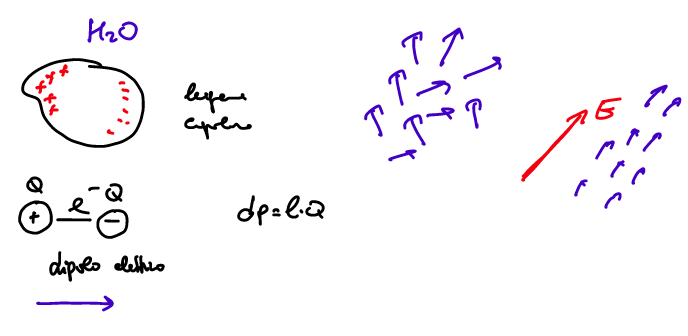
\includegraphics[scale=0.4]{immagini/pol_dip.png}
	\caption{Polarizzazione delle molecole a seguito dell'applicazione di un campo elettrico}
\end{figure}
\\\\Il mezzo viene quindi polarizzato per effetto del campo esterno.\\\\
\paragraph{Polarizzazione Ionica}
Nel corpo umano c'è tanta acqua, quindi è molto importante. Ci sono nel corpo altri materiali solidi, in cui è più difficile riconoscere la molecola in quanto sono organizzati sotto forma di reticolo, dove ogni nodo ha una composizione ionica e quindi una parte positiva ed una negativa ad esempio NaCl: l'Na si va ad "appiccicare" al Cl negativo.\\Nella singola cella, un pezzo è negativo ed uno è positivo, quando si applica un campo E, l'oggetto non può muoversi poiché vincolato, ma può essere deformato, quindi la poralizzazione ha effetto sulla modifica del reticolo, come riassunto nella figura sottostante
\begin{figure}[!h]
	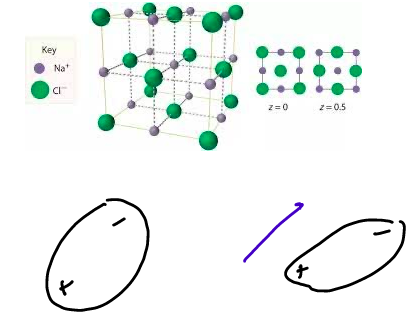
\includegraphics[scale = 0.5]{immagini/pol_io_effetti.png}
	\caption{Effetti della polarizzazione ionica}
\end{figure}
\paragraph{Polarizzazione elettronica}
Questa agisce direttamente sull'atomo, dove abbiamo il kernel positivo e la nube di elettroni. Anche in questo caso, in presenza di un campo E esterno la nube elettronica si può distribuire, su una forma magari più schiacciata, quindi abbiamo ancora un effetto dovuto allo stimolo esterno
\begin{figure}[!h]
	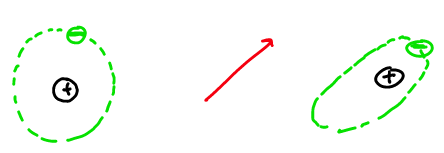
\includegraphics[scale=0.6]{immagini/pol_elettr_effetto.png}
	\caption{Effetti della polarizzazione elettronica}
\end{figure}
\\\\La dissipazione risulta nel momento in cui è necessario trasferire informazione, in quanto occorrono dei segnali sinusoidali, avremo che il campo esterno ha la seguente forma
\begin{figure}[!h]
	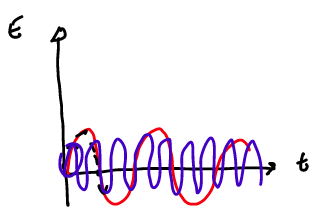
\includegraphics[scale=0.7]{immagini/appl_ce.png}
	\caption{Andamento nel tempo del campo elettrico generato da un segnale sinusoidale}
\end{figure}
\\\\questa applicazione di una forza elettrica alla struttura produce lavoro, siccome la materia vuole stare in un certo modo, la struttura tenderà ad opporsi allo stimolo e quindi ci sarà inerzia che produce attrito e che quindi conseguentemente verrà prodotto un riscaldamento.\\La dissipazione è quindi dovuta alla coesione complessiva dell'organismo che tende a non far muovere le molecole come vogliono.\\È simile a cosa accade con un forno a microonde: se metto del grasso non si cuoce bene, se lo metto in acqua questa cede il calore e lo fa riscaldare più velocemente.\\Se ci fosse una frequenza maggiore, ci sarebbe un ritardo in quanto il corpo umano ha del ritardo per capire che sta succedendo qualcosa e quindi le molecole sono sollecitate contro una forza, ci sarà quindi prima un po' di inerzia per cui ci vuole del tempo prima che la struttura si accorga che sta arrivando un fonte d'onda, ma finché se ne accorge arriva già il fronte negativo e quindi quello che avviene è che l'interazione con la materia è ridotta e concentrata sulla parte esterna.\\\\Occorre ora capire come rappresentare il corpo umano: si usa il modello di Debye, per cui abbiamo
\begin{equation}
	\dot{\epsilon} = \epsilon_{\infty} + \dfrac{\epsilon_s - \epsilon_{\infty}}{1 + j\omega \tau} 
\end{equation}
dove
\begin{itemize}
	\item $\epsilon_s$ è la costante statica (??)
	\item $\epsilon_{\infty}$è la costante ottima
	\item $\tau$ è il tempo di rilassamento, legato al tempo che serve alla molecola per sentire lo stimolo e tornare alla condizione iniziale dopo che lo stimolo è finito. È quindi il ritardo con cui viene seguito lo stimolo
\end{itemize}
Se rappresentiamo consideriamo una rappresentazione grafica:
\begin{figure}[!h]
	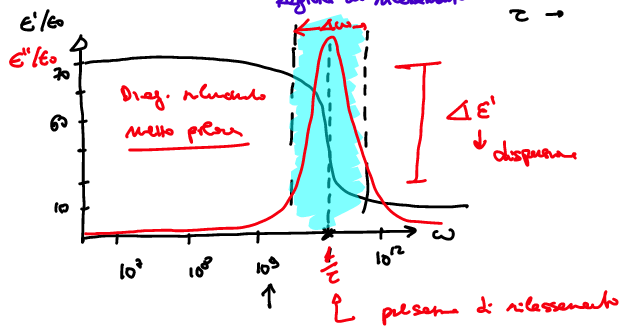
\includegraphics[scale=0.5]{immagini/eps_in_time.png}
	\caption{Andamento del rapporto $\frac{\epsilon'}{\epsilon_0}$ ed $\frac{\epsilon''}{\epsilon_0}$}
\end{figure}
\\\\teniamo conto che i GHz sono nell'ordine $10^9$, mettiamo ad $\frac{1}{\tau}$ la pulsazione di rilassamento.\\Avviene che la parte reale, quindi la capacità di immagazzinare energia e trasmetterla, in prossimità della frequenza in rosso ha un passaggio brusco, in un range di frequenza abbastanza stretto, la regione celeste che è la regione di rilassamento. La parte immaginaria ha un andamento totalmente opposto, in quella finestra c'è un assorbimento importante, le perdite sono elevate e quindi la potenza ceduta viene dissipata dal corpo. Questo è il digramma di rilassamento in un mezzo polare, le conseguenze da un punto di vista di comunicazione è nel che lavorare nella finestra celeste ci sono due fenomeni negativi:
\begin{itemize}
	\item molte perdite, se mando 1W di potenza buona parte del segnale è propagato;
	\item guardando alla permettività, mandando un segnale con una banda importante avrà ogni componente spettrale con una diversa velocità di propagazione e quindi avremo informazione dispersa
\end{itemize}
Quindi tutti i mezzi biologici sono dispersivi, quindi occorre lavorare distanti dalla zona di rilassamento perché il segnale ha effetti dispersivi e distorcenti.\\Visto invece dal punto di vista della fisioterapia, conviene lavorare in quella fascia perché c'è dissipazione e quindi riscaldamento.\\L'acqua ha una pulsazione di rilassamento dell'ordine di 20GHz, quindi il forno a microonde che funziona a 2450 MHz non è molto lontano.\\Questo avverrebbe se ci fossero solo composti polari come l'acqua, ma l'espressione quando consideriamo un corpo umano va adeguata a composti come proteine etc... ottenendo
\begin{equation}
	\dot{\epsilon} = \epsilon' - j \frac{\sigma}{\omega\epsilon_0} = \epsilon_{\infty} + \dfrac{\epsilon_s - \epsilon_{\infty}}{1 + (j \omega \tau)^{1 - \alpha}}
\end{equation}
(dove $0 < \alpha < 1$), 
ottenendo \textbf{l'espressione di Cole-Cole}.\\Mettendo tutto insieme, si è visto che tutto il corpo umano si può rappresentare con 4 di queste espressioni
\begin{equation}
	\dot{\epsilon} = \sum\limits_{i = 1}^{4} \dfrac{\epsilon_{si} - \epsilon_{\infty}}{1 + (j \omega \tau_i)^{1 - \alpha_i}} + \epsilon{\infty} - j \frac{\sigma_0}{\omega}
\end{equation}
dove tutti i parametri con la i e $\sigma$ sono dipendenti dai tessuti del corpo considerato.\\Rappresentando la finestra di dispersione, abbiamo 3 finestre per i vari parametri:
\begin{figure}[!h]
	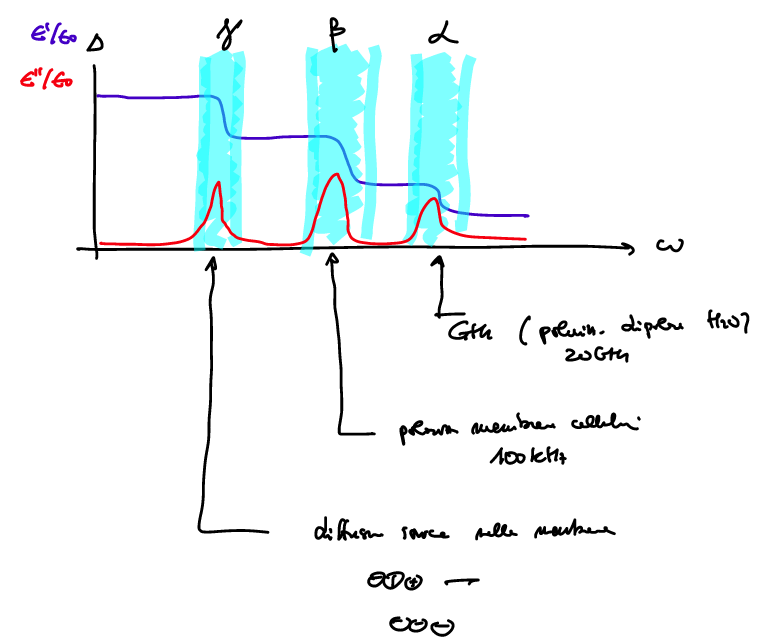
\includegraphics[scale=0.5]{immagini/fin_disp.png}
	\caption{Finestre di dispersione}
\end{figure}
\\\\nelle varie finestre ci sarà un incremento di perdite locale, questa è la risposta del corpo umano tessuto per tessuto (grasso, pelle, ...) in termini di riscaldamento, ed hanno nomi $\gamma$, $\beta$ $\alpha$, dove comandano diversi effetti
\begin{itemize}
	\item[$\gamma$] comanda la polarizzazione dipolare dell'acqua
	\item[$\beta$] comanda la polarizzazione delle membrane cellulari
	\item[$\alpha$] diffusione ionica nelle membrane
\end{itemize}
Immaginando di avere delle cariche libere: applicando il campo questi ioni entrano, poi applicandone un altro escono e quindi c'è assorbimento che produce delle perdite.
\subsection{Come caratterizzare i materiali}
Negli anni 90, sulla spinta dell'evoluzione della telefonia mobile, si è studiato l'impatto del telefono sulla testa e molti gruppi hanno studiato come caratterizzare i tessiti (sugli animali), usando l'espressione come interpolatore ed hanno estratto i parametri che sono di interpolazione. Ci sono dei DB dove in base alla frequenza ed al materiale c'è la lista dei parametri e quindi introducendola nella Cole-Cole generalizzata si ottiene la $\dot\epsilon$.\\Uno dei DB è Italiano, del CNR: niremf.ifac.cnr.it/emfref o /tissprop: si possono scaricare direttamente i parametri oppure avere i valori di permetività e conducibilità: otteniamo diversi valori tra cui la lunghezza d'onda ($\lambda = \frac{\lambda_0}{\sqrt[2]{\epsilon_r}}$). Prendendo ad esempio il muscolo, all'aumentare della frequenza, la conducibilità aumenta, la permettività diminuisce. Più c'è presenza di acqua, più permettività e conducibilità sono elevate.Ne riportiamo alcuni:
\begin{table}
    \begin{tabular}{c|c|c|c|c}
        Tessuto & 10 Mhz ($\frac{\epsilon_r}{\sigma}$) & 434 Mhz & 915 Mhz & 2450 Mhz\\
        \hline
        Grasso & 54 205 & 15 60 & 5 820 & 12 341\\
        Muscolo & 283 715 & 57 1120 & 55 1450 & 50 2272\\
    \end{tabular}
\end{table}
la differenza di conducibilità è importante, quindi il muscolo dissiperà sicuramente più potenza del grasso.
Cerchiamo ora di caratterizzare tutto da un punto di vista ingegneristico
\subsubsection{Assorbimento}
Un'onda arriva su un materiale: una grandezza importante è la densità di potenza dissipata nel corpo
\begin{equation}
	p_j = \frac{1}{2} \sigma \abs{E}^2
\end{equation}
e si misura in $\frac{W}{m^3}$.\\Per le norme di emissione si considera la SAR (Specific Absorption Rate), data da:
\begin{equation}
	SAR = \frac{p_j}{p}
\end{equation}
misurato in $\frac{W}{kg}$ e che indica quanta potenza viene assorbita per unità di massa del dispositivo, ed è quindi data da 
\begin{equation}
	\frac{\partial P}{\partial m} = \frac{1}{2\rho} \sigma \abs{E}^2
\end{equation}
e si usa in quanto è più facile da misurare.\\Se abbiamo un organo e vogliamo calcolare la potenza avremo quindi:
\begin{equation}
	P(\Omega_m) = \int\limits_{\Omega_m} P(r')SAR(r) dr'
\end{equation}
dove 
\begin{equation}
	SAR(\underline{r}) = \frac{1}{2 \rho(r)} \sigma(r) \abs{E(r)}^2 
\end{equation}
Le misure vengono fatte su dei "fantocci" che simulano le caratteristiche EM del corpo, il modo più semplice è usare acqua zucchero e sale:
\begin{itemize}
	\item l'acqua ha una permettività intorno a 70 Ghz
	\item il sale abbassa la $\epsilon_r$
	\item lo zucchero aumenta la $\sigma$
\end{itemize}
Ci sono delle ricette per ricostruire ogni organo e poter quindi misurare il SAR, altrimenti si usano fantocci da "macellaio", pezzi di carne etc...
\subsubsection{Propagazione nei tessuti biologici}
Consideriamo il caso più semplice possibile, dove il corpo umano è un mezzo omogeneo, avrà quindi una permettività $\epsilon' - j \frac{\sigma}{\omega}$.\\Immaginiamo di avere i due mezzi, (1) e (2) e che arrivi un campo elettrico che sia un'onda piana, si propaghi in direzione z, come mostrato in seguito:
\begin{figure}[!h]
	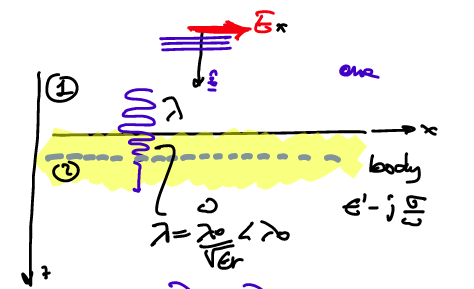
\includegraphics[scale=0.5]{immagini/es_propag.png}
	\caption{Esempio di propagazione di un'onda EM che attraversa due mezzi}
\end{figure}
\\\\Cosa accade al corpo: abbiamo, per un'onda piana
\begin{equation}
	E_x(z) = E_0 e^{-jkz}
\end{equation}
dove k è la costante complessa di propagazione
\begin{equation}
	k = \beta -j \alpha
\end{equation}
ed $\alpha$ e $\beta$ sono rispettivamente il fattore di propagazione ed il fattore di attenuazione:
\begin{equation}
	\alpha = \omega\sqrt[2]{\mu\epsilon'}\{ \frac{1}{2}[ \sqrt[2]{1 + (\frac{\epsilon^{\nu}}{\epsilon'})} -1] \}^{\frac{1}{k}}
\end{equation}
(esponente della quadra forse sbagliata).\\Sia $\alpha$ che $\beta$ dipendono dalla propagazione e dal mezzo.\\L'onda entra nel mezzo e man mano tenderà ad attenuarsi per via delle perdite, è importante capire da che punto in poi possiamo dire che l'onda si sia attenuata: definiamo $\delta_s$ = $\frac{1}{\alpha}$ ed è tale per cui z(profondità)= = $\delta_s$:
\begin{equation}
	\abs{\dfrac{E_x(\delta)}{E_y(\delta)}} = \frac{1}{e}
\end{equation}
che è circa del 37\%, quindi comunicare sotto questa soglia diventa molto complicato, la densità di potenza proporzionale al modulo di E si è ridotta invece del 13\%. Abbiamo un grafico come quello in \ref{sar_att}:
\begin{figure}[!h]
	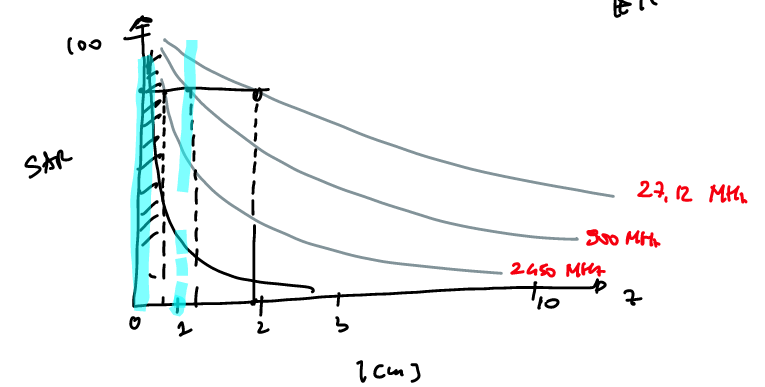
\includegraphics[scale=0.5]{immagini/attenuazione_sar.png}
	\caption{Attenuazione del SAR}
	\label{sar_att}
\end{figure}
\\\\supponiamo di fissare un valore di riferimento del SAR: questo sarà ottenuto nel mezzo, al variare della frequenza, ad una profondità via via crescente: se la profondità diminuisce lo spessore aumenta, quindi aumentando la frequenza otterremmo una profondità di penetrazione molto sottile.\\Fissando la profondità, all'aumentare della frequenza, il SAR tende ad abbassarsi quindi le conseguenze sono che volendo arrivare i profondità per comunicare con un dispositivo in profondità occorre usare frequenze basse, per cui il $\delta_s$ è basso, aumentando la frequenza l'interazione è sempre più in superficie \textbf{\textsf{(ricorda di smentire i coglioni che dicono che il 5G fa male perché entra nel corpo. COJONI, leggete le frequenze usate COJONI)}}.

\chapter{Lezione 3}
\section{Discontinuità fra due mezzi}
Cosa accade quando c'è una discontinuità: il corpo umano può essere rappresento in modo semplice come un mezzo non omogeneo, e quando l'onda incide il corpo umano sperimenterà una serie di effetti. Cosa accade quindi quando l'onda attraversa una superficie: consideriamo una superficie che separi due materiali differenti, materiale 1 e 2 ovvero grasso e muscolo: immaginiamo di avere determinati campi elettrici \underline{E} e di induzione \underline{D} e vediamo cosa succede alla potenza rilasciata sul corpo: la distribuzione della potenza dipende dall'incidenza dell'onda, possiamo avere campo elettrico paralleli o normale e dipendentemente dal fatto che il campo arrivi normale o parallelo avremo il \textbf{teorema di continuità dei campi}: a ridosso della discontinuità la componente tangente dei campi si conserva, quindi il campo parallelo sulla discontinuità $\pi$ si conserva senza avere salti, mentre la E$_\perp$ non si conserva, c'è un salto ma sappiamo che si conserva la componente D$_\perp$.\\Da queste considerazioni, cerchiamo di capire le conseguenze sulla distribuzione di potenza a ridosso delle superfici:
\begin{enumerate}
	\item Polarizzazione tangente:
	\begin{equation}
		\underline{E} = \underline{E_{\parallel}}
	\end{equation}
	avremo che 
	\begin{equation}
		P = \frac{1}{2}\sigma|E|^2
	\end{equation}
	e quindi le due P, una prima della superficie di separazione ed una dopo saranno 
	\begin{equation}
		p_1 = \frac{1}{2}\sigma_1|E_1|^2 p_2 = \frac{1}{2}\sigma_2|E_1|^2
	\end{equation} ne consideriamo il rapporto che sarà dato da
	\begin{equation}
		\frac{p_1}{p_2} = \frac{\sigma_1}{\sigma_2}
	\end{equation}
	\item Polarizzazione normale: ripartiamo da 
	\begin{equation}
		\frac{p_1}{p_2} = \dfrac{\frac{1}{2}\sigma_1|E_1|^2}{\frac{1}{2}\sigma_1|E_2|^2}
	\end{equation}
	dove le componente ortogonali NON sono più uguali come prima, quindi esprimiamo uno in funzione dell'altro: 
	\begin{equation}
		\epsilon_1 E_{\perp1} = \epsilon_2 E_{\perp2}
	\end{equation}
	ricaviamo $E_{\perp1}$ che messo nel rapporto fa si che questo dipenda anche dalla permettività:
	\begin{equation}
		\frac{p_1}{p_2} = \frac{\sigma_1}{\sigma_2} \abs{ \frac{\epsilon_2}{\epsilon_1}}^2
	\end{equation}
\end{enumerate}
Con degli esempi, CAPIAMO:\\ il mezzo 1 è grasso, mentre mezzo 2 è il muscolo. Fissiamo una frequenza fra quelle libere, f = 434 MHz e abbiamo $\epsilon_r$ e $\sigma$:
\begin{table}
	\begin{tabular}{|c|c|c|}
		& $\epsilon_r$ & $\sigma$\\
		muscolo & 60 & 1\\
		grasso & 15 & 0,1\\
		
	\end{tabular}
\end{table}
nella polarizzazione tangente, avremo che 
\begin{equation}
	p_f = \frac{1}{10} p_m
\end{equation} (dove f ed m sono fat e muscle), mentre nella nella polarizzazione ortogonale avremo 
\begin{equation}
	p_f = \frac{16}{10} p_m
\end{equation}
quindi si inverte: in un caso la potenza è maggiore nel muscolo, nell'altro caso nel grasso.\\Come sono gli andamenti:
\begin{figure}[!h]
	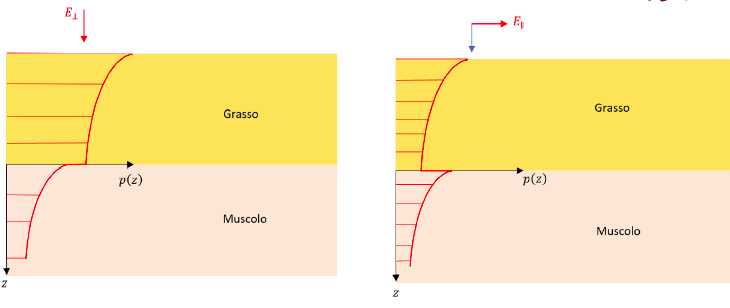
\includegraphics[scale=0.5]{immagini/disc_mezzi.png}
	\caption{Variazione di densità di potenza in base all'incidenza del campo E}
\end{figure}\\\\
la potenza man mano che si scende in profondità si attenua con legge esponenziale. Nel caso tangente, nella discontinuità, la potenza nel grasso è $\frac{1}{10}$ di quella nel muscolo, c'è un salto netto e poi continua a calare per via dell'attenuazione.\\Nel caso parallelo, c'è un salto ma in direzione opposta, perché in questo caso la potenza è maggiore nel grasso.\\L'effetto di assorbimento dei tessuti dipende quindi da come è fatto il dispositivo che genera il campo, in base a come lo genera: se normale, il valore nel muscolo è basso, mentre se parallelo è maggiore e quindi anche l'effetto di esposizione del corpo sarà differente.\\Vediamo ora l'effetto di questa potenza assorbita
\section{Effetti dell'assorbimento di potenza}
L'effetto principale è il riscaldamento ("effetto microonde"), quindi l'esposizione EM ha come effetto principale questo riscaldamento, che in alcuni casi come i sistemi terapeutici è voluto (sempre es. fisioterapia), in molti casi sono effetti collaterali, non voluti quindi si cerca di ridurli. Cerchiamo di capire il legame fra il SAR e la variazione di temperatura nel corpo: c'è l'equazione di Fourier che spiega come evolve un processo termico, che nel caso di una sorgente EM ha un pezzo in più
\begin{equation}
	\rho C \frac{\partial T(t)}{\partial t} = \Delta (K \Delta T) + p
\end{equation}
dove 
\begin{itemize}
	\item la temperatura T dipende da tempo e posizione (T(t, \underline{r}));
	\item $\rho$ è la densità (?)
	\item C è il calore specifico ovvero la quantità di calore assorbita da 1g di sostanza durante la variazione di temperatura di 1° ($\dfrac{J}{kgC°}$)
	\item K è il coefficiente di conducibilità termica
	\begin{equation}
		\frac{\Phi Q}{\Delta T} (\dfrac{W}{m°C})
	\end{equation}
	più k è elevato più il mezzo tende ad essere isolante. Infine p è la densità di potenza assorbita ($\frac{W}{m^3}$).\\ 
\end{itemize}
Ora, è molto più agevole considerare la stessa equazione quando dividiamo ambo i membri per $\rho$, in quanto
\begin{equation}
	\frac{P}{\rho} = SAR
\end{equation}
questo è il termine "forzante", questa diventa la sorgente del termine noto e quindi rilascia calore e tale potenza è una sorgente che si chiama \textbf{endogena}, in quanto è fornita all'interno del materiale mediante onda EM: se poggiamo un pezzo di metallo caldo su un oggetto, questa è una sorgente esogena, mentre questa si origina dall'interno.\\Nel corpo umano ci sono un paio di peculiarità:
\begin{itemize}
	\item è vivo, quindi si oppone a degli stress esterni, in questo caso il riscaldamento dell'onda EM col sangue che è un sistema di raffreddamento: il vaso si dilata ed il passaggio di sangue toglie calore. C'è un termine che si oppone al riscaldamento
	\item c'è poi un termine dovuto alla combustione chimica del cibo, che genera energia e si oppone
\end{itemize}
Otteniamo quindi la nuova equazione, Bioheat equation (Pennes 1948)
\begin{equation}
	\rho C \frac{dT(t)}{dt} = \Delta (k \Delta T) + p + M - B
\end{equation}
dove: 
\begin{itemize}
	\item M è il metabolismo ($\frac{W}{m^3}$), calore metabolico, \item B è la perfusione sanguigna, che ha segno meno perché tende ad opporsi per l'incremento dovuto agli altri termini.
\end{itemize}
Abbiamo che 
\begin{equation}
	B = W\cdot c_b (T - T_{arteria}
\end{equation}
dove T arteria se stiamo bene è di 37°, se questa diminuisce è il sangue che tende a scaldare, altrimenti raffredda. Ma dopo un po' c'è shock termico e quindi il tessuto comincia a bruciare: se ne vediamo l'andamento
\begin{figure}[!h]
	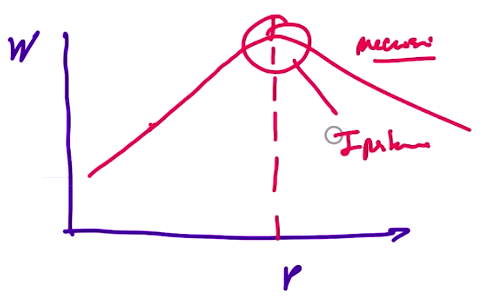
\includegraphics[scale=0.5]{immagini/andam_perf.png}
	\caption{Andamento della perfusione sanguigna, in funzione della densità di potenza}
\end{figure}

c'è un punto in cui va giù, ovvero quando la temperatura supera il 44° la perfusione sanguigna non ce la fa più perché il vaso non si più più estendere ed i tessuti necrotizzano (nel punto cerchiato si verifica l'ipertermia).\\Occorre quindi evitare che la temperatura inserita nel corpo dal dispositivo sia vicina ai 43°-44°, altrimenti si arriva a bruciare.\\Ci interessa l'equazione perché c'è un modo semplice per misurare il SAR: il cellulare rilascia un certo SAR nella testa, si parte dall'equazione di Pennes: il primo termine è istantaneo, poi c'è il termine di conduzione, la M quando c'è una sorgente esterna è piccolo rispetto al calore esterno ed anche la B è un fenomeno lento: il $\tau$ del fenomeno EM è veloce (ordine dei ns), se tocchiamo qualcosa di caldo non è istantaneo capire che si passa ad una temperatura fredda (ordine s), quindi applicando un fenomeno EM in un $\Delta t$ minore di un minuto nell'equazione rimane solo che 
\begin{equation}
	\rho C \frac{\partial T}{\partial t} \simeq p
\end{equation}
quindi dividiamo per $\rho$ ed otteniamo il SAR, che è proporzionale alla variazione di temperatura in un tempo abbastanza breve, quindi la posso approssimare come 
\begin{equation}
	C\frac{\Delta T}{\Delta t} \leq 1m
\end{equation}
Se mettiamo in una bacinella un liquido body-like (acqua zucchero sale) ed introduciamo un telefono cellulare, se facciamo una "foto" all'esterno (con termocamera o sondine), la zona sarà calda verso l'esterno e man mano sempre più fredda, così si può misurare il SAR prodotto dai dispositivi radianti.
\section{Normative EM}
Il progetto del dispositivo deve essere safety by design, quindi devo progettare prima il dispositivo che abbia fra i requisti una certa intensità di campo EM.\\Le attività del capire le soglie di esposizione nascono negli anni 80-90, l'impulso è stato dato dall'esplosione dei telefoni cellulari, c'è stato uno sforzo grande nel 97'-98' per capire quali parametri considerare e come caratterizzarli.\\Prima sono stati fatti degli studi con animali e tessuti espiantati e poi fatta una grossa analisi della letteratura scientifica. Sono stati poi fatti degli studi per cercare di correlare con le malattie (come tumori etc...), si è poi cercato di ridurre gli effetti accertati a breve termine, infine noti gli effetti gli studi si sono spostati sull'individuare le dosi soglia per evitare tali effetti.\\Ci sono due classi di effetti dell'esposizione ai campi EM:
\begin{enumerate}
	\item effetti diretti:
	\begin{itemize}
		\item accoppiamento con campi E a bassa frequenza
		\item accoppiamento con campi B a bassa frequenza
		\item assorbimento di energia EM.
	\end{itemize}
	Queste 3 tipologie di fenomeno producono due effetti percepibili:
	\begin{itemize}
		\item riscaldamento di organi e tessuti, ed è quella più facilmente quantificabile perché produce calore
		\item stimolazione di nervi e muscoli: c'è un disturbo dovuto al segnale, è possibile che il muscolo si contragga o che vengano stimolati degli effetti chimici e sono difficili da caratterizzare perché sono a lungo termine e sono più difficili da mettere in evidenza.
	\end{itemize}
	\item effetti indiretti, legati principalmente a
	\begin{itemize}
		\item alle correnti di contatto
		\item accoppiamento del campo EM con dispositivi impiantati, interazione con un dispositivo impiantato nel corpo. I primi pacemaker erano sensibili al telefono cellulare, sono stati poi protetti con dei filtri
	\end{itemize}
\end{enumerate}
Sull'analisi e la ricondizione degli effetti sono stati individuati dei limiti: inizialmente sono stati individuati i limiti di base, ovvero quelli legati alle grandezze EM che producono direttamente l'effetto, ovvero campo E nel corpo, al SAR ed in alcuni casi alla densità di potenza ovvero a grandezze direttamente generate nel corpo e che sono direttamente correlabili agli effetti diretti.\\Chiaramente cambiano in base alla frequenza, aumentandola, diminuisce la permettività sulla pelle.\\Misurarle è difficile, quindi sono stati introdotti degli \textbf{insiemi di livelli di riferimento o derivati}: sono delle grandezze che si possono valutare in assenza del corpo umano: se abbiamo un cellulare a contatto con la testa, leviamo la testa e calcoliamo le grandezze in un volume che sarebbe stato occupato dalla testa.\\Se scelti bene, rispettando i livelli di riferimento allora questi implicheranno che tali valori verranno rispettati anche quando sarà presente il corpo umano, MA NON vale il viceversa: se vengono rispettati i requisiti di base, non è detto che vengano rispettati quelli di riferimento.\\Le restrizioni di base sono quindi legate alla misurazione "in situ", mentre invece le restrizioni derivate sono misurate in assenza del corpo umano e quindi il loro rispetto implica i primi.\\Abbiamo ad esempio quelli per l'ELF fra 1-100 Khz
\begin{figure}[!h]
	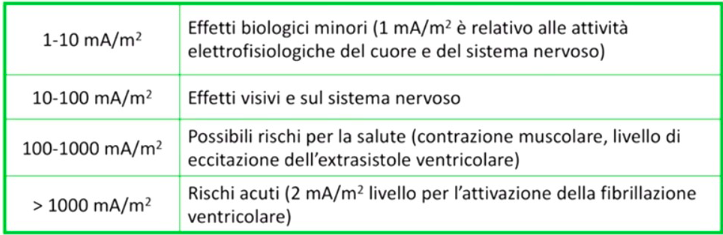
\includegraphics[scale=0.5]{immagini/elf_effetti.png}
	\caption{Effetti sul corpo umano in corrispondenza di Extremely Low Frequency}
\end{figure}
\\\\poi la microonde (100 Mhz in su), la sperimentazione animale indica come soglia di danno alla salute un incremento della temperatura di 1°C, per legarlo alla grandezza EM si è visto dalle misure che applicando un SAR per 6 min di 4 W/kg si innalza la temperatura di 1°C.\\I limiti di base del SAR sono diversi fra operatori e popolazione: un operatore può essere più esposto in quanto può prendere le dovute precauzioni, difatti per i lavoratori mediati su 6 min i valori sono circa 5 volte tanto, inoltre la media va fatta sui 10g: se ad un certo punto c'è un hotspot,  possibile superare il limite ma per un punto non posso buttare il dispositivo e quindi si fa una media su 10 g di materiale: si misurano i valori di SAR sui 10g e si fa questa media mobile così da buttare gli outlayers
\begin{figure}
	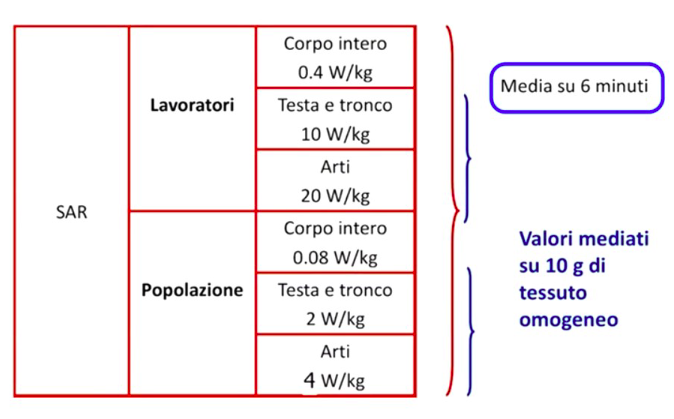
\includegraphics[scale=0.5]{immagini/limiti_sar.png}
	\caption{Limiti del SAR mediato su 6 minuti}
\end{figure}
\\\\Nel caso di dispositivi wearable, i limiti dei lavoratori sono coincidenti con quelli della popolazione\\Vi è poi un altro aspetto: le analisi vengono spesso fatte nel caso peggiore, ovvero quando viene trasmessa una sinusoide, quindi un segnale continuo.\\Nella realtà ogni dispotivo di telemetria ha un \textbf{duty cycle:} ci  sono parti alte e poi periodi di nulla, come mostrato in figura:
\begin{figure}[!h]
	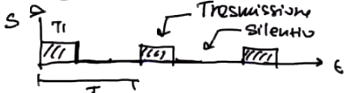
\includegraphics[scale=1.5]{immagini/duty_cycle.png}
	\caption{Trasmissione classica di un dispositivo di telemetria}
\end{figure}
\\\\Immaginiamo di avere un esempio in cui un dispositivo trasmette una volta l giorno lo stato di salute di una protesi impiantata, dove:
\begin{itemize}
	\item la trasmissione dura T = 1min;
	\item il SAR di picco è pari a 10 $\frac{W}{kg}$, quindi sopra soglia
\end{itemize}
averemo un minuto al giorno in cui il SAR è sopra soglia, ma facendo la media otteniamo 
\begin{equation}
	<SAR>_{6 min} = \frac{1}{6} \cdot 10 = 1,67 \frac{W}{kg}
\end{equation}
e quindi sotto la soglia di omologazione, avremo quindi un valore che è d $\cdot$ SAR.\\\\Se però un soggetto è portatore di oggetti come pacemaker i limiti vanno impostati per ogni istante di tempo: se viene messo in atto un attacco isico e si produce una potenza molto elevata, questo viene messo fuori uso.\\\\In Italia ed in Europa: il quadro italiano si pone in maniera molto restrittiva rispetto a quelle europee, dove in Europa sono indicati 40 V/m, in Italia ce ne sono 6. Inoltre, ovunque vanno rispettati certi valori, in siti come scuole etc.. ci devono essere valori ancora più bassi, inoltre a regime vanno rispettati dei valori ancora più bassi. La legislazione italiana fissa 3 livelli:
\begin{itemize}
	\item limite di esposizione: 20 V/m, non devono poter essere misurati in zone che non sono ad esempio dei tralicci recintati
	\item valore di attenzione: in alcuni ambienti dove ci si viva per un tempo maggiore di 4h consecutive non ci devono essere più di 6 V/m
	\item obiettivi di qualità: fare in modo che progressivamente in qualunque punto si vada verso i 6 V/m.
\end{itemize}
\subsection{Come fare una valutazione}
Ci si muove su tre livelli a complessità crescente:
\begin{enumerate}
	\item Misura del campo EM in assenza del corpo umano, andando a misurare i livelli di campo nel volume occupabile dall'uomo, si media per 6 min e si confrontano con i livelli derivati. Se rientrano nella normativa, possiamo omologare il dispositivo
	\item Se 1 da valori più elevati, occorre salire di complessità. Qui va fatta una simulazione EM, in cui si introduce il corpo umano, ma può andare bene un fantoccio di forme standard (cubi, cilindri), spesso di materiale omogeneo.\\Con un simulatore si simula il dispositivo e si calcolano campi e SAR nel fantoccio
	\item Se ancora i valori sono elevati, si fa una nuova simulazione con un modello antropomorfo, ovvero con tutti i tessuti del corpo umano con la sua permettività e conducibilità  e si valuta il SAR iterando ciascun componente del corpo umano.\\Se non si è conformi, tocca tornare alla progettazione.\\Esistono dei fantocci, il più famoso è visible human (progetto HUGO), un ergastolano che venne messo sotto gelatina, ghiacciato e fatto a fette e dopo la sedia elettrica venne "fotografato". È un fantoccio dove ci sono tutti i tessuti.
\end{enumerate}

\chapter{Lezione 4}
\section{Link bodycentrici - generalità}
Si fa riferimento a quei collegamenti nei quali in qualche modo compare il corpo umano, qui non solo c'è una sorgente che irradia, ma c'è un oggetto che si pone nel mezzo ed è molto complesso (corpo umano).\\Possiamo caratterizzare questi sistemi in base a 
\begin{itemize}
	\item[A)] orientamento della radiazione: immaginiamo di avere un corpo, possiamo avere un'antenna fuori che sta irradiando nel corpo oppure un'irradiazione che dal corpo irradia verso l'esterno.\\Possiamo quindi avere link:
	\begin{itemize}
		\item into the body, dove abbiamo ad esempio:
		\begin{itemize}
			\item sensori
			\item harvester: raccolgono l'energia esterna e la forniscono all'elettronica 
			\item sistemi di telemedicina: possiamo avere un dispositivo che cerca di interrogare dei sensori che sono all'interno del corpo
			\item terapia fisica, ovvero l'irraggiamento del corpo umano ai fini della terapia
		\end{itemize}
		\item out of the body (esterno), dove l'irradiazione dal corpo va verso l'esterno. Abbiamo:
		\begin{itemize}
			\item telemedicina, il sensore trasmette il dato verso l'esterno
			\item sensori
			\item trackers o beacon: dispositivi che servono per identificare la persona. Il dispositivo trasmette informazioni ad esempio sulla posizione
		\end{itemize} 
	\end{itemize}
	\item[B)] tipologia di interazione
	\begin{itemize}
		\item quasi statica, i campi E e B sono poco variabili nel tempo:
		\begin{itemize}
			\item induttivo, si lavora principalmente col campo B
			\item di tipo capacitivo, in cui si lavora col campo E 
		\end{itemize}
		\item zona di midfield, è una zona intermedia che domina molte delle applicazioni body centriche, non siamo più nel campo lontano ma non possiamo più separare campo elettrico e magnetico
		\item radiativa, abbiamo che i campi non sono più così separabili
	\end{itemize}
\end{itemize}
Immaginiamo di avere un elemento radiante, ed una corrente (antenna di cellulare, smartwatch etc...) ed avere r che è la distanza dominante: abbiamo 3 regioni
\begin{figure}[!h]
	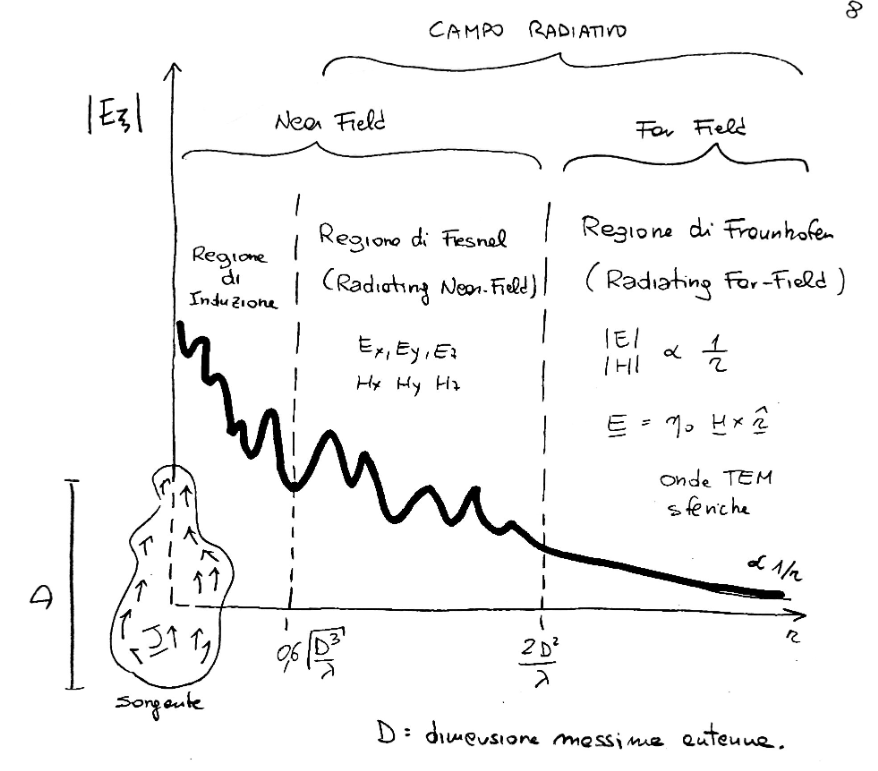
\includegraphics[scale=0.5]{immagini/regioni_campo.png}
	\caption{Regioni del campo radiativo}
\end{figure}
\\\\Nella zona di far field il campo elettrico e magnetico sono fra loro ortogonali, (anche a k che è la direzione di propagazione) e la densità di potenza è reale ed è proporzionale al campo elettrico, (copia tutte le formule)\\Nella zona induttiva, che è il near field, il campo varia molto lentamente e l'energia è induttiva(??) ma possiamo usarla per far colloquiare due dispositivi, ci sono tutte le componenti e sono mischiate e non si possono separare. Poi c'è la zona di mezzo dove comunque non si segue $\frac{1}{r}$.\\Va tenuto chiaro che: nelle zone vicine, quando abbiamo a che fare col corpo umano, c'è energia reattiva che  magnetostatica o elettrostatica che NON si propaga ma si può "raccogliere" ed accoppiare e quindi usare per le applicazioni.\\\\Un altro aspetto importante sono le frequenze di lavoro:
\begin{itemize}
	\item basse, Low Frequency ed High Freqeuncy (kHz - MHz), le LF vanno 30-300 KHz, mentre HF 2-30MHz. Sono tipiche dei sistemi quasi statici, quando lavoriamo con queste stabiliamo un regime quasi statico e quindi tutto interviene in campo quasi statico. Qui il campo si attenua di meno quando interagisce col corpo, lo spessore pelle è maggiore ma sono coinvolti dei dispositivi più grandi. Se volessi con una sola antenna trasmittente leggere tante antenne del corpo umano dovrei usare queste frequenza
	\item elevate, UHF e microwave. Le UHF sono 300 MHz - 3GHz, mentre le microvawe sono da 1 - 3GHz.  Sono tipiche dei sistemi radiativi. Penetrano meno, circa 4cm nel corpo e quindi possono interagire con la pelle meglio (penetrano meno) ma hanno come vantaggio di permettere l'utilizzo di antenne più basse.
	\item 
\end{itemize}
L'antenna è un oggetto poco miniaturizzabile, quindi in molti dispositivi l'ingombro è dovuto alla presenza di antenne (similmente a quanto accade per la batteria) soprattutto se l'antenna deve essere piccola.\\\\Altro aspetto importante sono le geometrie, i layout
\begin{itemize}
	\item in dispositivi quasi statici, abbiamo 
	\begin{itemize}
		\item coil, avvolgimenti nei sistemi magneto-statici
		\item piastre, che svolgono la funzione di condensatore
	\end{itemize}
	\item in sistemi radiativi abbiamo
	\begin{itemize}
		\item dipoli
		\item loop
		\item slot
		\item patch
	\end{itemize}
\end{itemize}
Seguono poi le tipologie di servizio, ovvero perché usiamo il sistema bodycentrico:
\begin{itemize}
	\item comunicazione: uno degli scopi principe.\\Sistemi wearable, con cui è possibile fare delle body area network. Ad esempio, in ambito militare, quando vanno in missione c'è una rete mash fra i vari soldati: ognuno ha una radio che permette di stabilire una comunicazione con gli altri fino ad arrivare al capo
	\item telemetrica e comando: abbiamo un dispositivo sul corpo o al suo interno, che deve mandare un messaggio all'esterno (telemetria). Il comando invece serve principalmente a configurare dei dispositivi impiantati: le pompe ad infusione, dispositivi che rilasciano farmaco, neuro-stimolatori periodicamente vanno controllate dagli esperti del settore (\textbf{\textsf{NON NOI}}).
	\item Wireless Power Trasnfer: trasferimento di energia per alimentare un dispositivo che non ha batteria o per evitare che la batteria di un dispositivo venga consumata per comunicare.\\Anche se un dispositivo medico non ha la batteria si cerca di non usarla i più possibile, quindi l'energia che serve per comunicare viene fornita dall'esterno.\\L'esempio classico è la ricarica del cellulare o dello spazzolino elettrico
	\item Marker / Labeling: alcuni dispositivi medici possono essere dei \textbf{marcatori}. I marker non trasmettono informazione, ma servono ad esempio per centrare il corpo umano rispetto a qualche altra sorgente.\\Il labeling è l'associazione al dispositivo medico un codice, simile al codice a barre, fatto a radiofrequenza da sistemi RFID quindi si può assegnare un identificavo ad un oggetto per leggere e scrivere dentro. Si fa quindi identificazione e tracking, ma anche localizzazione.
\end{itemize}

\subsection{Architetture di comunicazione}
Abbiamo due modalità per stabilire un link:
\begin{itemize}
	\item link simmetrici
	\item link asimmetrici
\end{itemize}
differiscono sostanzialmente nella gerarchia con cui uno trasmette ed uno riceve, c' è differenza nei protocolli usati, nella progettazione hadrware etc...

\subsubsection{Link simmetrici}
In un link in generale abbiamo due oggetti, A e B che devono scambiarsi delle informazioni.\\In un link simmetrico, possiamo definire trasmettitore TX e ricevitore RX: TX manda il segnale ed RX deposita tale segnale su un carico.\\È possibile anche che si scambino i ruoli fra i due ad un certo punto, quindi non parlano mai contemporaneamente (half duplex).
\begin{figure}
	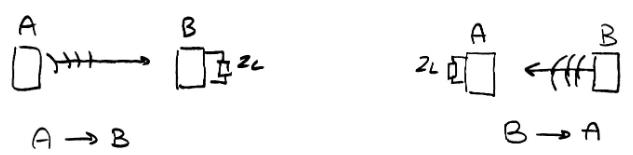
\includegraphics[scale=0.5]{immagini/com_halfd.png}
	\caption{Schema di comunicazione half duplex}
\end{figure}\\\\
L'esempio classico sono il cellulare che parla con stazione RB e poi altro cellulare, o anche i walkie talkie.\\Ambe due i dispositivi hanno la stessa elettronica e serve una fonte locale di alimentazione, quindi o una alimentazione ad un cavo fisico oppure una batteria.\\Esempi: bluetooth BT, che funziona a 2450 MHz, bluetooth BLE (low energy) che permette di avere una durata della batteria più lunga: la prima cosa da fare è il pairing fra i dispositivi.\\LTE (ex 4G), che è Long Term Evolution, 850-900 - 2100 MHz, ci sono i sistemi UMTS, CDMA, SCDMA\\Wi Fi, le cui frequenze sono 2450 - 5800\\5G, che ha diverse frequenze, 700 MHz, LTE, 3600Mhz, 26GHz fino a 60 GHz.\\Sistemi IoT: LoRa (Long Range) e SIGFOX: sono sistemi di Wireless Lan, sistemi con cui interconnettere oggetti e quindi molto usati in sistemi di IoT, possono collegarsi ad un hotspot tipo WiFi ma con range molto più alto e con batterie che durano molto tempo (ordine anni). Le frequenze sono più basse, 433 Mhz e 868 Mhz.

\subsubsection{Link asimmetrici}
Altra filosofia, che è molto gerarchizzata: tipicamente c'è un oggetto che si chiama lettore (Reader) che va ad interrogare un altro oggetto "stupido" da un punto di vista dell'elettronica e risponde per riflessione, quindi non ha sensori ma in qualche modo riflette il segnale modulandolo in modo da poter codificare i valori 0 ed 1. 
\begin{figure}
	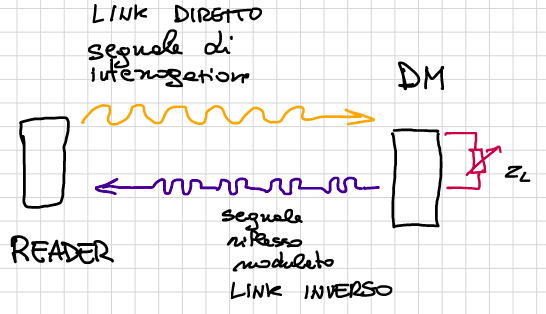
\includegraphics[scale=0.5]{immagini/com_fulld.png}
	\caption{Schema di comunicazione full duplex}
\end{figure}
Per farlo, c'è un interruttore del D che permette di modulare ma è molto semplice e non richiede batteria o elettronica complessa, tutta l'energia che serve per attivare l'interruttore arriva dal trasmettitore, a differenza invece del Reader.\\Ci sarà un link diretto dal lettore al trasmettitore e poi un link inverso che va dal dispositivo al reader.\\In questo caso i due dispositivi possono mandare segnali contemporaneamente, quindi con comunicazione full duplex. Abbiamo dispositivi monouso, come cerotti che evitano l'uso di batterie e costano meno.

\subsection{Efficienza dei collegamenti}
Quando si fa un collegamento, una delle cose più preziose è l'energia, in quanto sistemi wearable non possono essere collegati alla corrente e quindi tutta l'energia è data dalla batteria che non ha durata lunga, inoltre nel corpo umano si perde tanta energia per via delle perdite.\\Introduciamo in due step:
\begin{itemize}
	\item[1] solo antenna che trasmette in prossimità del corpo umano, ad esempio l'orologio che prova a collegarsi al wifi: abbiamo il corpo, un dispositivo che sta irradiando e che produce una radiazione che poi entra magari nel corpo.\\Consideriamo poi una superficie che racchiude tutto:
	\begin{figure}
		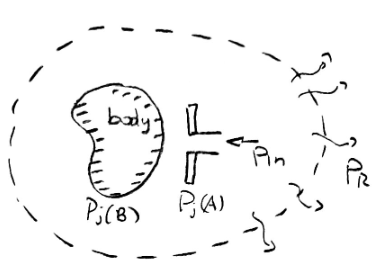
\includegraphics[scale=0.3]{immagini/eff_coll_1.png}
		\caption{Schema di trasmissione}
	\end{figure}\\\\
	potremmo applicare il thm di Pointying, abbiamo della potenza irradiata, della potenza dissipata nel corpo (P$_j$), quindi la potenza totale che fornisco è 
	\begin{equation}
		P_{in} = P_r + P_j(k) + P_j(B) + P_j(A)
	\end{equation}
	se abbiamo un sistema di comunicazione deve prevalere la potenza irradiata, mentre invece per sistemi che fanno terapia deve prevalere quella dissipata.\\\\Possiamo caratterizzare la bontà del trasmettitore in base alla efficienza 
	\begin{equation}
		\ni_R = \frac{P_R}{P_{in}} = \dfrac{P_r}{P_j(A) + P_j(B)} \equiv \dfrac{R_R}{R_R + R_j}
	\end{equation}
	abbiamo in più il termine (verde) che è proprio specifico della presenza del corpo.Si possono anche associare le resistenze delle antenne.\\Quando non c'è il corpo umano, la $R_R$ tende ad andare proporzionalmente come il raggio dell'antenna, l'andamento è simile a questo (metti immagine), le prestazioni migliorano ingrandendo l'antenna in modo da avere una resistenza di radiazione migliore ed enfatizzare quindi la parte radiata.\\Se abbiamo anche il corpo, aumentando le dimensioni dell'antenna irradia meglio ma manda più potenza nel corpo e ci sarà maggiore dissipazione. Se $\frac{R}{\lambda}$ aumenta abbiamo due effetti opposti:
	\begin{itemize}
		\item da una parte aumenta la resistenza di radiazione
		\item ma da una parte aumenta anche la resistenza di perdita
	\end{itemize}
	(copia ASSOLUTAMENTE L'IMMAGINE DEL DONDOLO)-\\Nei sistemi radianti, non comanda la lunghezza in se, ma la lunghezza RISPETTO alla lunghezza d'onda. Abbiamo il seguente andamento:\\ ad un certo punto, superato questo, il dispositivo irradierebbe come uno piccolo e quindi sarebbe poco efficiente.\\È un tradeoff e vale ogni volta che abbiamo un mezzo con perdite (pelle, pneumatico, etc...) l'effetto di portare un dispositivo in prossimità di un mezzo avrà un valore ottimale e tale valore ottimale dipende poco dalla forma dell'antenna (dipolo, loop, slot) ma tanto dalla forma: gli oggetti fatti a loop hanno una l$_{max}$ ottimale in termini di ingombro.
	\item[2] Consideriamo ora anche il link in presenza del corpo umano.\\Possiamo avere la seguente immagine:\\un'antenna che irradia, chiamiamo P$_l$ la potenza che verrà raccolta per far funzionare il dispositivo. Il parametro che descrive quanto p efficiente questo trasferimento di potenza dal tx all'oggetto è il PTE: $\frac{P_L}{P_{in}}$ e va massimizzato per avere un link efficiente.\\Dipenderà anche in questo caso dai tessuti, dalla posizione rispetto al corpo (più in profondità, maggiore l'attenuazione), dipende anche dalla forma delle antenne coinvolte ed ovviamente dalla frequenza (PTE tende a diminuire quando la frequenza aumenta perché l'attenuazione del corpo aumenta ed è quindi più difficile eseguire il comportamento).\\Possiamo scrivere $P_L = P_{in} \cdot PTE$, fissando la PTE, per aumentare la P$_L$ va aumentata la $P_{in}$, ma nel corpo aumenta anche il SAR ovvero la potenza rilasciata: qui il problema è che per aumentare la P$_L$ potremmo aumentare la potenza in ingresso ma se aumenta troppo il SAR sforo i limiti di legge e qui si capisce bene cosa vuol dire safety by design.\\Il primo anello della catena di progettazione deve:
	\begin{itemize}
		\item SAR $< SAR_{max}$
		\item P$_{in}$ < P max
	\end{itemize} 
	viene quindi fuori un vincolo per la PTE, imposto dal SAR: questo ci dice quindi quanto deve essere fatto bene il collegamento in modo da poter minimizzare la potenza necessaria.
\end{itemize}

\section{Link in near field}
Negli anni di fine 800 (1831) vengono fatti i primi studi da Faraday sulla induzione EM: gli studi avevano a che fare con due coil, in modo che questi potessero trasferirsi energia senza che questi si toccassero. L'accoppiamento veniva fatto mediante l'uso di materiale ferromagnetico, per molti anni venne usato ad esempio nei trasformatori ma non per la comunicazione.\\Agli inizi del 1900 ci sono gli esperimenti di Hertz e di Tesla, dove si parla proprio di trasmissione di informazione a distanza, Telsa introdusse anche i concetti di risonanza in quanto la sua ambizione era rifornire l'energia nelle città tramite una torre che mandava energia sulle case della città.\\Sono applicate nelle comunicazioni a bassa frequenza e piccola distanza, in ambito medico abbiamo dispositivi IMD (Implanted Medical Device) che possono essere pacemaker, defibrillatori, neurostimolatori etc... la comunicazione viene stabilita con un altro coil messo sulla superficie del body stabilendo un link a bassa frequenza. Sono link di tipo quasi statico, basati o su accoppiamento induttivo, o su accoppiamento induttivo risonante o accoppiamento capacitivo. Le frequenze di lavoro sono le HF ed LF, anche attorno ai KHz: in queste condizioni la capacità di conduzione del corpo è bassa, quindi basse perdite che permettono di avere PTE elevata, inoltre la permettività è elevata.\\I dispositivi non sono vere e proprie antenne, sono una specie di elettrodi in quanto lavorano in campo vicino.
\chapter{Lezione 5}
\section{Inductive (Magnetic) coupling}
Nell'accoppiamento siamo nel regime delle LF (125 KHz) e delle HF(13-56 MHz)
e possiamo usarlo per dispositivi medici impianti ma anche per la ricarica wireless.\\Tipicamente vengono usati due coil, di cui uno fa da trasmettitore ed uno raccoglie il campo vicino, siamo in campo vicino e non si può parlare di antenne:\\
\begin{figure}[!h]
	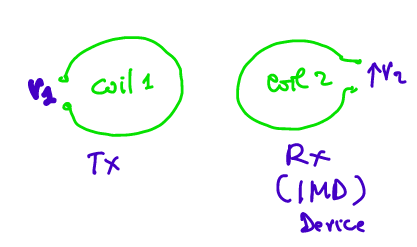
\includegraphics[scale=0.7]{immagini/spire.png}
	\caption{Coil usati per l'accoppiamento magnetico}
\end{figure}\\\\
abbiamo due spire ai capi della seconda spira vogliamo raccogliere la tensione.Parliamo di link induttivo perché avviene per induzione di Farady o magnetico perché avviene per il passaggio del campo da un coil all'altro, a noi interessa anche come sistema di comunicazione: questo sistema funzionerà come un trasformatore
 \\
 \begin{figure}[!h]
 	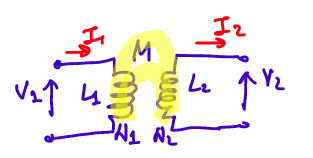
\includegraphics[scale=0.7]{immagini/trasf.png}
 	\caption{Sistema di comunicazione}
 \end{figure}\\\\
(M è il coefficiente di mutuo accoppiamento) ed abbiamo 
\begin{equation}
	\frac{V_1}{V_2} = \frac{N_1}{N_2}
\end{equation}
\begin{equation}
	\frac{I_1}{I_2} = \frac{N_2}{N_1}
\end{equation}
ed inoltre
\begin{equation}
	V_2 = -M \frac{dI_1}{dt}
\end{equation}
nel caso ideale abbiamo che tutto il flusso del primario è raccolto dal secondario e quindi vale:
\begin{equation}
	M = \sqrt{L-1 \cdot L_2}
\end{equation}
nel caso reale invece abbiamo:
\begin{equation}
	M = k \sqrt{L-1 \cdot L_2}
\end{equation}
dove k è il \textbf{coefficiente di accoppiamento}, e vale k $\in [0,1]$.\\
Vogliamo vedere come esprimere M per il sistema di due coil che sarà poi quello che legherà la tensione nel device rispetto alla tensione accesa nel primario:\\se c'è un filo lineare percorso da una corrente I\\
\begin{figure}[!h]
	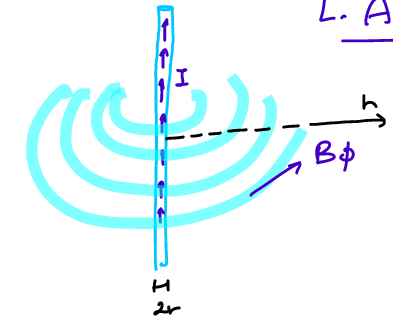
\includegraphics[scale=0.6]{immagini/corrente_filo.png}
	\caption{Campo magnetico generato da un filo lineare}
\end{figure}\\\\
viene generato un campo magnetico e dalla \textbf{legge di induzione di Ampere} abbiamo
\begin{equation}
	\underline{B} = \frac{\mu_0 I}{2 \pi r}\Phi
\end{equation}
se "curviamo" questo filo otteniamo questa configurazione
\begin{figure}[!h]
	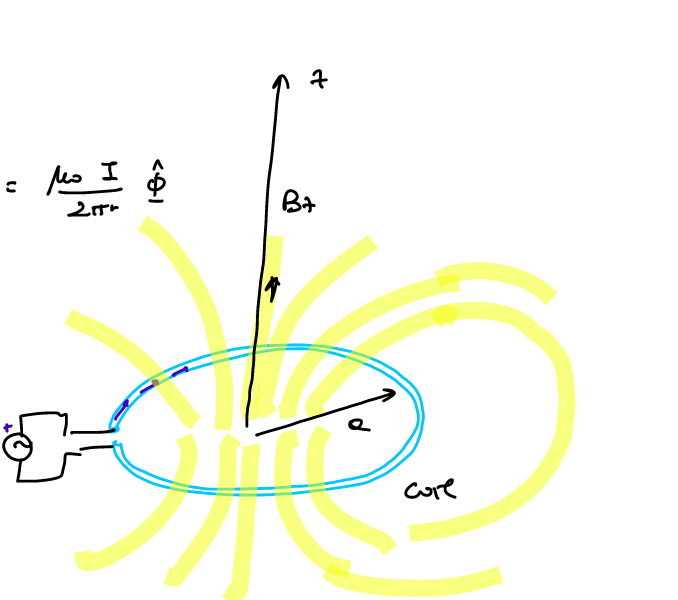
\includegraphics[scale=0.6]{immagini/solen.png}
	\caption{Campo magnetico generato da un filo lineare curvato}
\end{figure}
mettiamo un generatore in modo che scorra una corrente nel verso mostrato, allora verrà generato un campo magnetico le cui linee di forza sono come mostrate, considerando la $B_z$ che sarà
\begin{equation}
	B_z = \frac{\mu_0 I a^2}{2(a^2 + r^2)^{\frac{3}{2}}}
\end{equation}
se supponiamo di avere N spire, l'espressione precedente viene moltiplicata per N.\\Si vede intanto che se la distanza è r $>>$ a, allora $(a^2 + r^2) \approx r^2$, quindi avremo un andamento come $\frac{1}{r^3}$ e quindi il campo più forte si avrà nelle vicinanze ed avremo che $B_z$ si può approssimare con
\begin{equation}
	B_z = \frac{\mu_0 NI a^2}{2}\frac{1}{r^3}
\end{equation}
\\\\Consideriamo ora due coil, uno che trasmette ed uno che riceve \\
\begin{figure}
	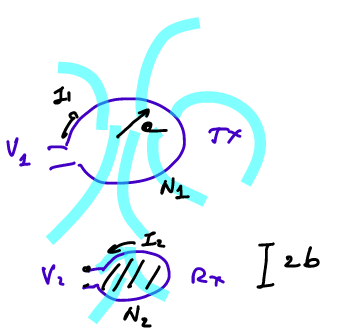
\includegraphics[scale=0.6]{immagini/coils.png}
	\caption{Sistema di due coil (tx ed rx)}
\end{figure}
\\\\avremo che RX concatenerà alcune delle linee del campo magnetico e quindi vale la \textbf{legge di Faraday}, che dice che un campo magnetico B variabile nel tempo che concatena una spira chiusa andrà ad indurre una ELF (Forza Elettromotrice Indotta) (vedi bene).\\Se consideriamo il flusso $\phi$ del campo magnetico:
\begin{equation}
	\phi(t) = \int\int \underline{B}(t) \cdot d\underline{s}
\end{equation}
allora la EMF sarà 
\begin{equation}
	V_2 = -N\frac{d\phi}{dt}
\end{equation}
c'è un meno perché la tensione che viene indotta ai capi nel secondario a sua volta tende a muovere degli elettroni che genera un campo magnetico che si oppone al primo (altrimenti si violerebbe il principio di conservazione).\\La applichiamo al nostro caso:
\begin{equation}
	V_2 = -N_2 \frac{d}{dt} \psi_{2,1} = -N_2 \frac{d}{dt} \int\int\limits_{S_2} \underline{B_1} da
\end{equation}
dove il pedice a destra è la causa, quello a sinistra è l'effetto (coil 2, coil 1), sostituiamo poi l'espressione per B (supponendo che i due coil siano colinerari, quindi allineati rispetto a z) ottenendo:
\begin{equation}
	V_2 = -N_2 \frac{d}{dt} \int\int\limits_{S_2} \frac{\mu_0 I_1 a^2 N_1}{2(a^2 + r^2)^{\frac{3}{2}}} da
\end{equation}
supponendo che i coil siano piccoli, possiamo considerare che il campo sia costante sul coil, possiamo integrare e moltiplicare per l'area:
\begin{equation}
	V_2 = -[] \frac{dI}{dt}
\end{equation}
e la confrontiamo con la $V_2$ ottenuta dalla precedente, quindi M è $f(N_1\cdot N_2, b^2, \frac{1}{r^3})$.\\\\Cosa succede invece se il TX e l'RX non sono allineati: supponiamo di avere un angolo $\alpha$ fra i due assi, il secondario raccoglierà meno flusso e quindi possiamo tenere conto della mutua rotazione con un cos($\alpha$), ottenendo un'espressione più completa di M aggiungendo il cos($\alpha$)
\begin{equation}
M = 	\dfrac{\mu_0 I a^2 N_1}{2(a^2 + r^2)^{\frac{3}{2}}} \pi b^2 cos\alpha
\end{equation}
\\\\Per incrementare il trasferimento di potenza fra un coil e l'altro possiamo:
\begin{enumerate}
	\item aumentare l'intensità del campo \underline{B}, ma viene limitato dai limiti del campo a basse frequenze
	\item possiamo diminuire la distanza fra tx ed rx, ma non è una cosa che si può fare sempre, ad esempio per un dispositivo medico impiantato
	\item aumentare la frequenza del campo \underline{B}, in modo che l'attenuazione sia meno evidente. La derivata nel dominio armonico è un -j$\omega$ ma l'aumento della corrente ha delle contro-indicazioni. Abbiamo $\frac{dI}{dt}$ $\rightarrow$ -j$\omega$I (quindi $V_2$ aumenta) ma questo fa si che ci siano più perdite e si dissipi di più (più potenza)
	\item aumentare il flusso concatenato, ovvero fare in modo che il secondario raccolga più possibile del primario che tipicamente si ottiene facendo in modo che il primario ed il secondario abbiano le stesse dimensioni oppure facendoli lavorare per \textbf{risonanza}.\\Anche qui occorre fare i conti con le normative di esposizione
\end{enumerate}
\subsection{Accoppiamento induttivo risonante}
Uno dei modi è quindi fare un'accoppiamento induttivo risonante: si deve a Telsa, alla risonanza si ha tipicamente un massimo trasferimento di potenza (o quanto meno di stimolo).\\Per far risonare i due sistemi occorre, innanzi tutto fare in modo che il tx sia risonante: occorre agire sulle dimensioni in modo che la parte immaginaria x sia pari a 0.\\Sull'RX c'è poco margine, se abbiamo un loop piccolo e ne vediamo la reattanza in ingresso $X_{in}$ se 2$pi$B << x allora la reattanza sarà induttiva, ovvero $>$ 0 e si comporterà come un circuito.\\Ci sarà poi il carico del dispositivo, ovvero qualcosa che gli permetta di utilizzare l'energia, occorre aggiungere un condensatore che può essere messo sia in serie che in parallelo.\\Avremo quindi il coil trasmittente e possiamo mettere in risonanza sia tramite un condensatore in serie oppure con un condensatore in parallelo 
\begin{figure}[!h]
	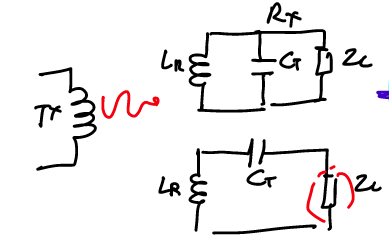
\includegraphics[scale=1]{immagini/cond_ser_parall.png}
	\caption{Condensatore in parallelo o in serie per il ricevente}
\end{figure}
 entrambe danno la stessa potenza sul carico ma cambiano i valori mutui di corrente e di tensione:
 \begin{itemize}
 	\item lo schema in parallelo darà corrente bassa e tensione elevata
 	\item lo schema in serie il contrario
 	tipicamente si sceglie il parallelo: dopo il carico, c'è tipicamente un rettificatore AC$\rightarrow$DC e poi deve esserci un convertitore da corrente alternata a corrente continua per alimentare la circuiteria digitale (l'elettronica).
 \end{itemize}
Questo tipo di dispositivo lavora meglio con alte tensioni, quindi si preferisce usare uno schema parallelo.\\\\Abbiamo quindi il nostro modello circuitale TX ed RX:
\begin{figure}
	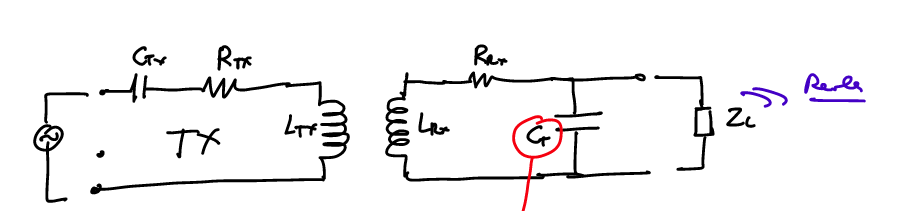
\includegraphics[scale=1]{immagini/schema_circuitale.png}
	\caption{Schema circuitale di TX ed RX}
\end{figure}
dove nel ricevitore C$_T$ è il condensatore di tuning. La $C_T$ va scelta in modo tale che 
\begin{equation}
	f_0 = \frac{1}{2\pi\sqrt{L_{R_x} \cdot C_T}}
\end{equation}
Abbiamo trovato che
\begin{equation}
	V_2 = -N_2 \frac{d}{dt} \int\int\limits_{R} \underline{B} ds
\end{equation}
passando al dominio dei fasori, sappiamo che $\frac{d}{dt} = j\omega$ ed abbiamo quindi 
\begin{equation}
	V_2 = -N_2 j\omega B_0 S_{RX} cos\alpha Q_{RX}
\end{equation}
in più compare il fattore di qualità Q del ricevitore, dove è definito come 
\begin{equation}
	Q_{RX} = \omega \frac{\Xi_{RX}}{P_{j, RX}}
\end{equation}
Più Q è elevato e meno potenza dissipata ci sarà e quindi più quella che viene immagazzinata.\\Per fare quindi in modo che aumenti $V_2$ occorre avere un fattore di qualità elevato che si ha quando il sistema è risonante, ancora di più se in parallelo.\\Avere un Q elevato comporta una criticità operativa, ovvero la banda è stretta in quanto la larghezza di banda è 
\begin{equation}
	B \propto \frac{1}{Q}
\end{equation}
(quanto più è alto il fattore di qualità tanto più c'è sensibilità a spostamenti dalla frequenza di lavoro).\\\\Con la $V_2$, quando questa è maggiore di una tensione di threashold che è connesso al coil primario, il secondario si accende e comincia a funzionare, quindi $V_2$ deve essere $> V_{th}$ e fissata la distanza sappiamo quali sono il fattore di qualità da avere etc... che sono valori minimi.\\Un parametro di performance che ci interessa è la \textbf{PTE (Power Trnasfer Efficiency)}, definita come 
\begin{equation}
PTE = \frac{P_L}{P_{in}}	
\end{equation}
quindi la 
\begin{equation}
	(1-PTE)P_{in}	
\end{equation}
è quella persa.\\È stato trovato che la PTE è data da:
\begin{equation}
	PTE = [1 + \frac{1}{q} + \dfrac{1}{M^2 Q_{TX} + Q_{RX}}(2 + q + \frac{1}{q})]^{-1}
\end{equation}
 \textbf{IMPORTANTE: QUESTO GROSSO GOAT DI MARROCCO TI FA PORTARE IL FORMULARIO (KING)}), dove q è dato da:
\begin{equation}
	q = \sqrt{\dfrac{1 + M^2\cdot Q_{TX}\cdot Q_{RX}}{1 + M^2 \cdot Q_{TX} Q_{RX}^{-1}}}
\end{equation}
e vale per un circuito risonante parallelo.\\Nota importante: a frequenza basse (dove siamo) le perdite dei tessuti sono basse, cioè la conducibilità $\sigma$ (legata alle perdite) è piccola. Siamo nell'ordine dei 100KHz e contano quasi più le perdite sui conduttori che sul tessuto.\\Tipicamente quindi i due coil conviene farli di dimensioni simili in modo che buona parte del campo B prodotto dal primario viene raccolto dal secondario, in alcuni casi però non è possibile farli simili perché magari un coil ricevente deve poter raccogliere più coil tx, quindi è possibile usare un coil booster:\\
\begin{figure}
	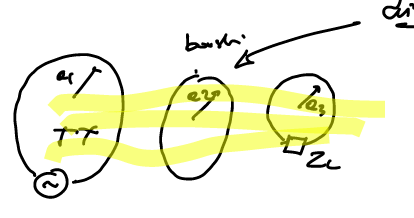
\includegraphics[scale=1]{immagini/booster_coil.png}
	\caption{Sistema con coil booster}
\end{figure}
\\\\
il booster ha dimensioni intermedie fra i due, è a corto circuito ed ha l'effetto di ridirezionare il flusso verso coil più piccoli.\\Funziona come un \textbf{direttore di antenna}, in modo che se il coil è piccolo ed in un posto difficilmente raggiungibile possiamo usare un coil intermedio in modo che venga ridirezionato il flusso fino a dove serve.
\subsection{Criticità}
Principalmente legata la disallineamento: immaginiamo di avere la classica stratificazione, col dispositivo IMD (copia disegno)\\l'ideale sarebbe avere il coil che trasmette in un certo punto, ma una volta impiantato non posso più vederlo, per cui se abbiamo un disallineamento non concateno più il massimo del campo e quindi avremo un notevole decadimento delle prestazioni.\\Una soluzione è porre dei magneti con opportune polarità in modo che il campo prodotto di polarizzazione fra i due magneti vada a far allineare i coil, quindi si possono impiantare dei micromagneti sotto pelle sia sul tx che sull'rx\\Altra criticità è la flessibilità: in molte applicazioni, soprattutto quando il dispositivo deve aderire a delle protesi o a degli organi, viene realizzato con un'elettronica flessibile, si può realizzare su delle membrane.\\Immaginiamo di avere il coil "spalmato" su qualcosa che può flettersi, ma questo provoca un cambiante nella forma che provoca un detuning: cambia il fattore di qualità e si abbassa la tensione raccolta.\\L'oggetto va quindi progettato a priori per quelle condizioni.\\Ultimo punto, riguarda i materiali.Essendo a frequenze basse, le perdite sui conduttori pesano e quindi servono conduttori con perdite basse come il rame, che però non è biocompatibile. Oggetti biocompatibili sono il titanio, che non è però un buon conduttore (1.5 ordini in meno del rame) e quindi tende ad avere perdite maggiori.\\Si può usare il rame andando a fare un coating, ovvero un rivestimento del conduttore di rame con materiale biocompatibile, come ad esempio
\begin{itemize}
	\item silicone
	\item materiali ceramici, che vanno bene per dispositivi solidi
	\item poliammide (PEEK il più usato, polimero semi cristallino), sono polimeri ovvero materiali fatti da tanti monomi agglomerati che formano una matrice molto solida
	\item zirconia
\end{itemize}


\subsection{Comunicazione del ricevitore col trasmettitore (modulazione capacitiva)}
Per la comunicazione inversa si può usare un link simmetrico, quindi si invertono le parti oppure si usa un link asimmetrico (come si tende a fare sempre di più) cioè il ricevitore va a modificare l'accoppiamento col trasmettitore ovvero fa quella che si chiama una \textbf{modulazione capacitiva}: si fa in modo che il sensore vada con una logica binaria a modificare l'accoppiamento col primario così che questo si renda conto che qualcosa sta irradiando dall'altro lato.\\Consideriamo il circuito di prima:\\
\begin{figure}[!h]
	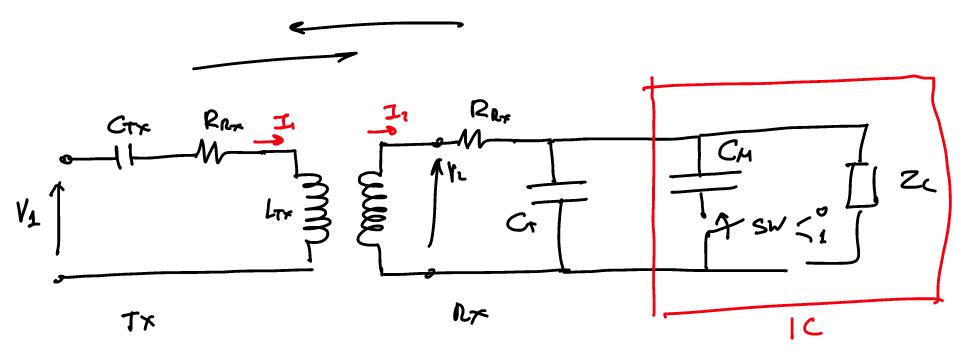
\includegraphics[scale=0.5]{immagini/schema_mod_cap.png}
	\caption{Schema per la modulazione capacitiva}
\end{figure}
\\\\
abbiamo poi un altro pezzo, una scatola dove troviamo un altro condensatore che si può connettere / sconnettere con interruttore (sarà il condensatore di modulazione) e quindi sarà il blocco che esegue tale modulazione, sarà un circuito integrato.\\Lo switch ha due stati, 0 o 1 (chiuso aperto) ed in base a questo il $V_1$ vedrà una cosa o un'altra:
\begin{itemize}
	\item switch open: bit '0', $V_1$ sarà dato (risolvendo il circuito) nel dominio dei fasori 
	\begin{equation}
		V_1 = \frac{1}{j \omega G_X} I_1 + j \omega L_{TX}I_1 + R_{TX}I_1 - j\omega M I_2^{(0)}
	\end{equation}
	e dove la frequenza è pari alla frequenza di risonanza
	\begin{equation}
		f_0 = \frac{1}{2\pi \sqrt{L_{RX} \cdot C_T}}
	\end{equation}
	abbiamo poi che il circuito è risonante e quindi il valore visto è alto, perché l'accoppiamento è forte.\\Ripuliamo quindi i termini reattivi in quanto siamo in risonanza
	ottenendo
	\begin{equation}
		V_1^{(0)} = R_{TX}I_1 - j\omega M I_2^{(0)}
	\end{equation}
	\item switch close: bit '1', abbiamo la somma dei due condensatori, di tuning e di modulazione e quindi avremo una $f_1$ diverso dalla frequenza di risonanza:
	\begin{equation}
		f_1 = \frac{1}{2\pi \sqrt{L_{RX}(C_T + C_M)}} \neq f_0
	\end{equation}
	 I due coil quindi non si parlano bene perché non sono in risonanza e quindi la $V_1$ vista dal primario sarà bassa
	 \begin{equation}
	 	V_1^{(1)} = R_{TX}I_1 -j\omega MI_2^{(1)}
	 \end{equation}
\end{itemize}
governando lo switch secondo elettronica digitale (apri/chiudi) facciamo in modo che $V_1$ sia modulato in ampiezza in quindi ottenere una situazione di questo tipo: vogliamo mandare questa stringa, sul writer si vedrà un qualcosa del genere:\\
\begin{figure}[!h]
	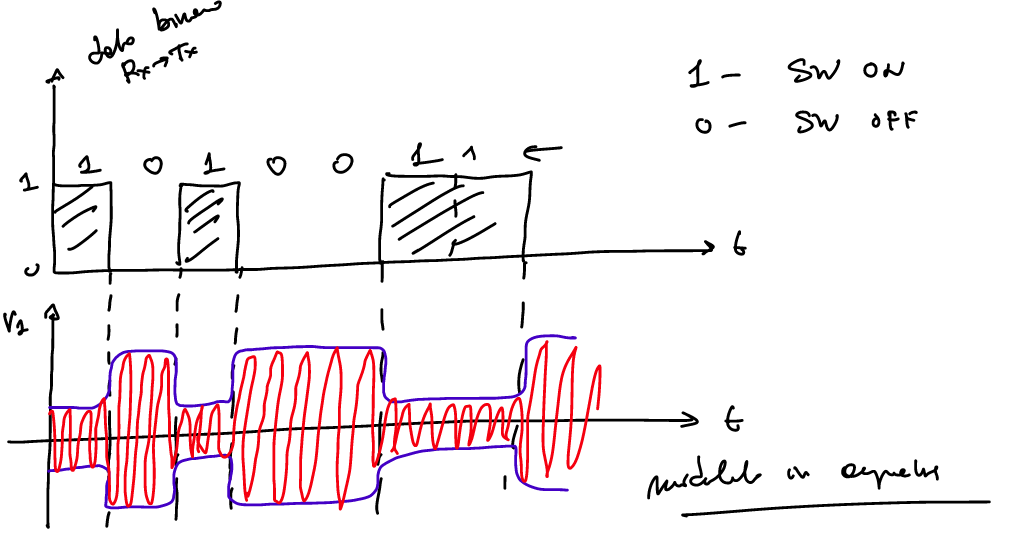
\includegraphics[scale=0.5]{immagini/rx_verso_tx.png}
	\caption{Segnale di risposta del ricevente}
\end{figure}\\\\
dove abbiamo il segnale modulato in ampiezza.\\Questo è il sistema con cui funzionano i sistemi NFC.\\È il primo collegamento in campo vicino visto, usato sia in ambito medico che anche in campo logistico, basato su coil:
\begin{itemize}
	\item patenti
	\item codice fiscale
\end{itemize}
tutto funziona esattamente così.


\chapter{Lezione 6}


\section{Near-field: link capacitivi}
Sono dei link meno usati degli altri ma hanno dei risvolti interessanti. Lavorano a frequenze un po' più alte, sui pochi MHz, ma se le dimensioni sono piccole si può anche arrivare al GHz.\\Immaginiamo un condensatore a facce piane e parallele, immaginiamo che sia alimentato da un generatore \\
\begin{figure}[!h]
	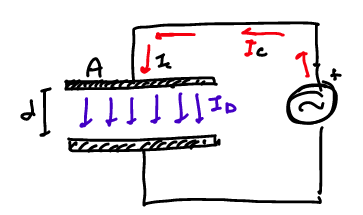
\includegraphics[scale=0.7]{immagini/circ_cap_link.png}
	\caption{Esempio di circuito}
\end{figure}\\\\
la corrente gira sul filo, il circuito ha un interruzione ma la corrente circola poiché viene generata una corrente di spostamento fra le facce del condensatore (legata al campo che si propaga e che carica il condensatore).\\La $I_d$ sarà
\begin{equation}
	\epsilon_0 \epsilon_r A \frac{\partial\underline{E}}{\partial t}
\end{equation}
oppure nel dominio dei fasori
\begin{equation}
	j\omega \epsilon_0\epsilon_rA\underline{E}
\end{equation}
Possiamo immaginare di avere il condensatore a cavallo del corpo umano, così, da poter mandare un'informazione alla piastra dentro.\\Si divide il condensatore a metà, su ogni faccia di esso, collegandola come segue
\begin{figure}[!h]
	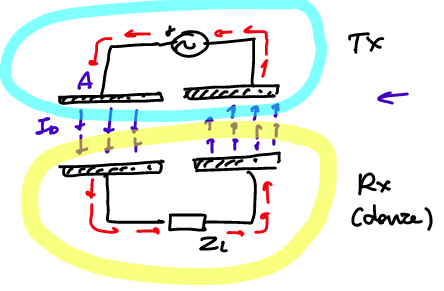
\includegraphics[scale=0.5]{immagini/divisione_circ.png}
	\caption{Divisione del circuito}
\end{figure}
le correnti faranno lo stesso giro di prima, abbiamo quindi due oggetti separati:
\begin{itemize}
	\item il primo è fatto con le due metà della prima faccia, sarà il tx
	\item il secondo è fatto dalle due metà dell'altra, sarà per noi il rx
\end{itemize}
il dispositivo deve quindi avere due elettrodi belli larghi che userà per accoppiarsi elettrostaticamente con i due elettrodi del ricevente.\\L'accoppiamento come detto è principalmente elettrostatico, quindi domina il campo E.\\Occorre però fare attenzione:
\begin{figure}[!h]
	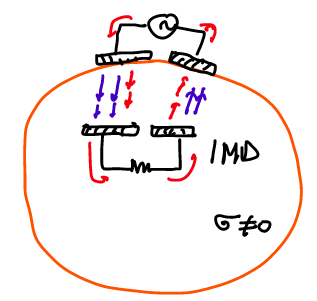
\includegraphics[scale=0.6]{immagini/circ_divis_corpo.png}
	\caption{}
\end{figure}
fra le due coppie di armature non abbiamo solo la corrente di spostamento, il mezzo corporeo ha una conducibilità $\neq 0$, quindi ci saranno anche delle correnti di conduzione che sono legate al fatto che il materiale permette di spostare anche elettroni.\\Nuovamente ci sono due fenomeni contrastanti:
\begin{itemize}
	\item propagazione, legato alle correnti di spostamento;
	\item dissipazione, legato alle correnti di conduzione.
\end{itemize}
Cerchiamo di caratterizzare le due entità:
\begin{itemize}
	\item $I_d = \epsilon_0 \epsilon_r A \frac{\partial\underline{E}}{\partial t}$
	\item la corrente di conduzione è data dalla legge di Ohm: abbiamo il body \\
	\begin{figure}[!h]
		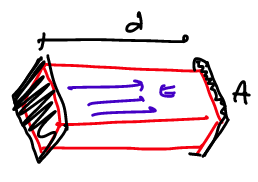
\includegraphics[scale=0.7]{immagini/rapp_body.png}
		\caption{Rappresentazione di un blocchetto di corpo}
	\end{figure}\\\\
	la resistenza del blocchetto è $R = \frac{1}{\sigma} \frac{d}{A}$, quindi $I_c = \frac{V\sigma(\omega)A}{d}$
\end{itemize}
come facciamo ad enfatizzare la corrente di spostamento:
\begin{itemize}
	\item se aumentiamo il campo E:
	\begin{itemize}
		\item possiamo aumentare la $V_0$ del generatore, ma se il campo aumenta dobbiamo fare attenzione ai limiti di esposizione
		\item ridurre d, ovvero la distanza fra le due armature così che il campo sia più intenso. Ma ci sono delle limitazioni legate all'istallazione
		\item aumentare l'area A delle placche (degli elettrodi), anche qui un punto di attenzione è l'ingombro per dispositivi impiantati
	\end{itemize}
	\item incrementare la frequenza, poiché la $I_d $pro a $j\omega$ (che è la derivata rispetto al tempo nel campo dei fasori), ma l'aspetto critico sono le perdite nei tessuti
\end{itemize}
Per ridurre la $I_c$ occorre fare l'opposto di quello che si faceva prima:
\begin{itemize}
	\item ridurre l'area A, ma si riduce anche la $I_d$
	\item ridurre la tensione di eccitazione del condensatore ma di nuovo si riduce anche l'altra
\end{itemize}
come sempre va trovato il compromesso in base all'applicazione, occorre effettuare una trade off analysis delle cose.
\subsection{PTE (Power Transfer Efficiency) e SAR}
Per analizzare la PTE si fa un circuito equivalente tenendo conto che ora le perdite nei tessuti non sono così trascurabili (verso i MHz le perdite sui tessuti sono più importanti di quelle sui conduttori). Facciamo quindi questo circuitino equivalente\\
\begin{figure}[!h]
	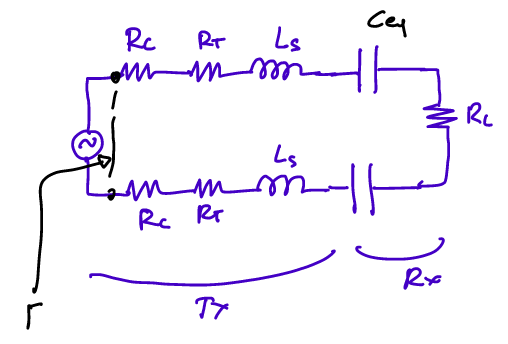
\includegraphics[scale=0.5]{immagini/circ_equiv.png}
	\caption{Circuito equivalente}
\end{figure}\\\\
(ogni resistenza fa riferimento alle perdite!!): il filo è approssimabile bene con l'induttanza in genere, possiamo assumere che le $R_C <<R_T$. C'è una formula che dice che la PTE (rapporto fra la potenza rilasciata sul carico e la potenza in ingresso) è 
\begin{equation}
	PTE = \frac{R_L}{R_L + R_T} (1 - \abs{\gamma}^2)
\end{equation}
e stesso vale per 
\begin{equation}
	R_T = R_L [\dfrac{d}{A \epsilon_0 \epsilon_r}]
\end{equation}
Quindi la PTE complessivamente aumenta se:
\begin{itemize}
	\item  aumenta la A
	\item diminuisce la d
\end{itemize}
quindi elettrodi larghi e dispositivi molto vicini.\\Vediamo come è correlata la massima potenza di tx immissibile nel dispositivo rispetto al SAR: sappiamo che il SAR è limitato: 
$
SAR_{max} =
\begin{cases}
	2 \dfrac{W}{kg} & \text{per testa e addome}\\
	4 \dfrac{W}{kg} & \text{per testa e addome} negli arti
\end{cases}$
Per legare il SAR alla potenza massima:
\begin{equation}
	PTE = \frac{P_L}{P_{TX}}	
\end{equation}
considerando 
\begin{equation}
	P_{TX}(1-PTE)	
\end{equation}
questa è la potenza che viene dissipata nel corpo, ovvero la $P_j$, quindi PTE*P$_{TX}$ è proprio la potenza ceduta al corpo mentre quella dissipata è l'altra.\\Consideriamo 10g di tessuto:

$P_j(10g) = \int\int\limits_{10gr} SAR dm$, ammettendo il SAR costante perché il volume è piccolo, possiamo ottenere $SAR * 10^{-2}$ W, quindi $P_jmax (10gr) = SAR_{max}10?{-2}$ che è la massima potenza che si può rilasciare in una massa di 10g.\\Facciamo un ipotesi brutale: immaginiamo che tutta la potenza venga rilasciata in un paio di cubetti di 10gr, quindi la max potenza rilasciabile in 20g è : $2*10^{-2}SAR_{max}$ che è molto conservativa come ipotesi perché la potenza viene distribuita su un volume maggiore.\\Allora la $P_jmax(20g) = P_{TX}(1-PTE)$ da cui la $P_{TX_{max}} = 2*10^{-2}SAR_{max}/1 - PTE$, quindi se il SAR è 2 $\frac{W}{kg}$ otteniamo un $P_{j_{max}} = \frac{0.04}{1-PTE} W$, nella testa ed addome, mentre negli altri avremmo $\frac{0.08}{1-PTE} W$.\\Quindi se la PTE fosse il 50\%, ma in realtà tipicamente è molto più bassa, avremmo circa 0.1W di P$_{TX}$ che può suonare bene (da quindi un'ordine di grandezza di riferimento).

\subsection{Criticità}
La criticità è simile a quella dell'accoppiamento induttivo ovvero i disaccoppiamenti, i due condensatori tendono a chiudere meno bene le correnti è c'è una perdita di efficienza di trasferimento.\\Il campo lavora su delle discontinuità, quindi nel grasso come ricordiamo (è poco vascolarizzato) c'è maggiore (vedi sopra).\\


\section{Link nel mid-field}
Fin ora abbiamo visto link a frequenze molto basse, aumentandola i dispositivi sono più lontani e non si può più approssimare ad elettrostatico o magnetostatico, siamo quindi nel midfield (regione di Fresnell, non siamo così lontani).\\Quando siamo a frequenza maggiori del GHz, e tipicamente più piccole dei 3GHz le perdite del corpo sono più alte, quindi $\sigma_{body}$ è più alta ma ci spostiamo qui perché se la frequenza è più elevata:
\begin{itemize}
	\item c'è un vantaggio nel bitrate, posso trasmettere informazioni più velocemente
	\item gli oggetti possono diventare elettricamente più grandi e quindi possiamo usare anche più oggetti contemporaneamente e quindi usare degli array di trasmettitori nel corpo
\end{itemize}
\textbf{RICHIAMO}: ciò che comanda nel mondo delle antenne non è la lunghezza l del dispositivo ma la sua dimensione elettrica che è $\frac{l}{\lambda}$ e la lunghezza d'onda nel vuoto è $\lambda_0$ ma in un mezzo con perdite è $\lambda_0/\sqrt{\epsilon_r}$ e quindi se abbiamo aria e sotto un mezzo biologico, se arriva un onda con una certa $\lambda_0$, quando entra nel mezzo la lunghezza d'onda diminuisce perché viene divisa per il valore di permettività del mezzo.\\Quindi all'aumentare della frequenza, siccome $\lambda_0 = \frac{\lambda}{f}$ la lunghezza fisica del dispositivo è 
\begin{equation}
	L_e = \frac{L}{C}f \sqrt{\epsilon_r}	
\end{equation}
quindi abbiamo un dispositivo elettricamente più grande pur rimanendo piccolo, quindi abbiamo un maggiore controllo sul campo EM irradiato.\\La lunghezza EM è 
\begin{equation}
	L_e \propto f\sqrt{\epsilon_r}
\end{equation}
e la frequenza migliore si ha per 1GHz, ovvero l'efficienza di un'antennina impiantata anche tenendo conto delle perdite è quella ottimale e vale nell'ipotesi in cui $D_{IMD} > 1cm$ e si ottiene la frequenza alla quale l'oggetto impiantato risulta efficiente come antenna.\\\\Abbiamo come altro vantaggio di poter usare più di un dispositivo:\\
\begin{figure}
	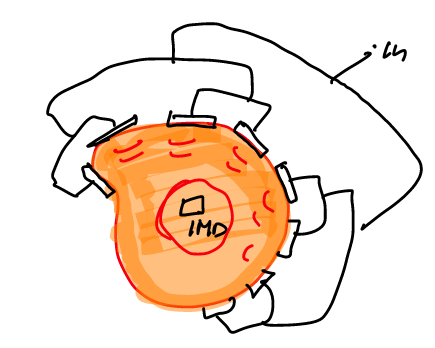
\includegraphics[scale=0.5]{immagini/disp_imp.png}
	\caption{Disposizione di vari dispositivi impiantati sul corpo}
\end{figure}
\\\\possiamo usare vari tipi di trasmettitori all'esterno che, siccome la frequenza è elevata, sono geometricamente piccoli ma elettricamente più grandi.\\Possiamo quindi collegarli con una rete di fascio, mandano un segnale in ingresso posso far si che ciascuno irradi un campo solo nel punto dove serve, quindi per focalizzare l'interrogazione in una piccola regione e si può fare perché gli oggetti sono piccoli geometricamente ma grandi (e quindi posso farli risonanti) elettricamente.\\Il vantaggio è che ognuno produrrà un SAR più basso, riuscendo quindi a rimanere entro i limiti delle normative.\\I conti sono complicati, non possiamo usare i concetti di guadagno delle antenne etc... quindi si introduce un modo di lavorare che non necessita approssimazione ma si rinuncia al rappresentare tutti i fenomeni: introduciamo il \textbf{guadagno di trasduzione}

\subsection{Guadagno di trasduzione (Transducer Power Gain)}
Il guadagno di trasduzione tiene conto di vari fatti ed è specifico per una configurazione particolare.\\Per ottenerlo, dobbiamo rappresentare l'antenna come una rete a due porte: immaginiamo di avere due antenne una che tx ed una che rx\\
\begin{figure}
	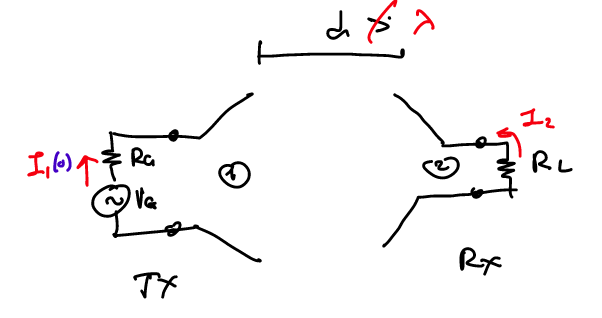
\includegraphics[scale=0.5]{immagini/rete_dp.png}
	\caption{Rappresentazione di un'antenna come rete a due porte}
\end{figure}
\\\\le antenne sono vicine, la distanza d non è più grande di $\lambda$ e quindi c'è disturbo.\\Occorrerebbe fare un calcolo del campo e della tensione raccolta, ma ci interessa analizzare il link di comunicazione, quindi che succede sul carico del ricevitore quando alimentiamo il trasmettitore: immaginiamo di rappresentare tutto come una scatola che verrà analizzata solo ai morsetti\\
\begin{figure}
	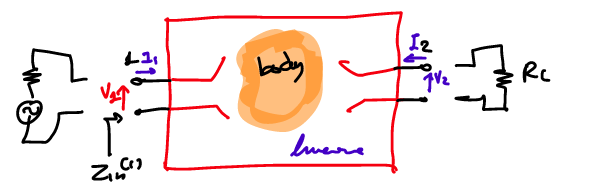
\includegraphics[scale=0.5]{immagini/antenna_scatola.png}
	\caption{Rappresentazione dell'antenna come una "scatola chiusa"}
\end{figure}
\\\\guardando quindi tensione $V_1$ e corrente, che consideriamo entrante nella rete $I_1$ e le $V_2$ ed $I_2$. Non perdiamo nulla perché dipendono dalle interazioni EM che stanno "dentro la scatola", che sono le osservabili.\\Consideriamo che il sistema sia lineare, possiamo immaginare che la tensione che vediamo ad una porta sia $V_1 = I_1$, guarderemo il seguente sistema:
$
\begin{cases}
	V_1 = I_1(0) Z_{11} + Z_{12}I_2\\
	V_2 = I_1(0) Z_{21} + Z_{22}I_2\\
\end{cases}
$
la corrente viene considerata sul punto di alimentazione, da cui la valutazione in 0 (ma la corrente tipicamente scorre ovunque).\\I coefficienti Z sono la \textbf{matrice di impedenza}\\\\
$
\begin{bmatrix}
	Z_{11} & Z_{12}\\
	Z_{21} & Z_{22}\\
\end{bmatrix}
= [Z]
$
\\\\dove i coefficienti sulla diagonale corrispondono al caso in cui si misura la corrente sulla porta 1 quando la porta 2 è in circuito aperto e viceversa, ovvero:
\begin{equation}
	Z_{ii} = \frac{V_i}{I_i}\bigg\rvert_{I_j = 0}
\end{equation}
\\Gli altri due coefficienti sono uguali se la rete è \textbf{reciproca}:
\begin{equation}
	Z_{ij} = Z_{ji} = \frac{V_i}{I_j}\bigg\rvert_{I_i = 0}
\end{equation}
ed sono \textbf{l'impedenza mutua} ed è il termine che da l'accoppiamento fra le due porte.\\L'impedenza in ingresso alla porta 1si esprime come 
\begin{equation}
	Z_{in}^{(1)} = \frac{V_1}{I_1} = Z_{11} + Z_{12}\frac{I_2}{I_1}	
\end{equation}
quindi la dipendenza è mediante il termine di impedenza mutua che da l'accoppiamento, e vale anche il viceversa 
\begin{equation}
	Z_{in}^{(2)} = \frac{V_2}{I_2} = Z_{22} + Z_{21}\frac{I_1}{I_2}
\end{equation}
\\Immaginiamo alcuni casi
\begin{itemize}
	\item[1)] L'antenna rx è chiusa in corto circuito\\
	\begin{figure}
		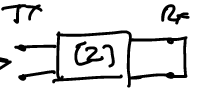
\includegraphics[scale=0.7]{immagini/rx_cortoc.png}
		\caption{Ricevente chiuso in corto circuito}
	\end{figure}
	\\\\L'impedenza che vedo è $Z_{in}^{(1)}$, se $V_2 = 0$ possiamo calcolare 
	\begin{equation}
		\frac{I_2}{I_1} = - \frac{Z_{21}}{Z_{22}}	
	\end{equation}
	e quindi avere  
	\begin{equation}
		Z_{in}^{(1)} = Z_{11} -\frac{Z_{12} \cdot Z_{21}}{Z_{22}} = Z_{11} -\frac{Z_{12}^2}{Z_{22}}	
	\end{equation}
	Quando questo avviene l'oggetto alimentato è fortemente infastidito dalla presenza dell'oggetto non alimentato
	\item[2)] L'antenna rx è in circuito aperto: la configurazione è la seguente\\
	\begin{figure}
		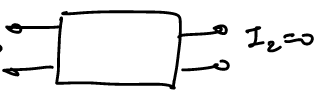
\includegraphics[scale=0.7]{immagini/ric_aperto.png}
		\caption{Antenna ricevente in circuito aperto}
	\end{figure}
	\\\\avremo $I_2 = 0$ e vediamo la $Z_{in}^{(1)}$, dall'espressione di prima viene cancellato un termine e quindi 
	\begin{equation}
		Z_{in}^{(1)} = Z_{11}	
	\end{equation}
	e possiamo dire che l'impedenza in ingresso sia simile a quella dell'antenna se fosse isolata.\\Normalmente in queste condizioni l'antenna tx risente poco della rx (a meno che questa non siamo molto grande).\textbf{IMPORTANTE: la $Z_{11}$ NON rappresenta l'impedenza dell'antenna isolata, ma è molto simile sopratutto se l'antenna ricevente è piccola.}
	\item[3)] Il caso più generale è quando RX è collegato ad un carico $Z_L$, $Z_{in}^{(1)}$ si ricava in quanto esistono diverse rappresentazioni circuitali:
	\begin{itemize}
		\item a $\pi$;
		\item a T
	\end{itemize}
	che hanno le stesse relazioni di grandezze in uscita di una rete a due porte, è dimostrabile (\textsf{\textbf{ma io credo al prof sulla parola}}).\\La rete più semplice è quella a T, una rete a T che ha la stessa matrice di impedenza di una rete a due porte ha questi valori:\\
	\begin{figure}
		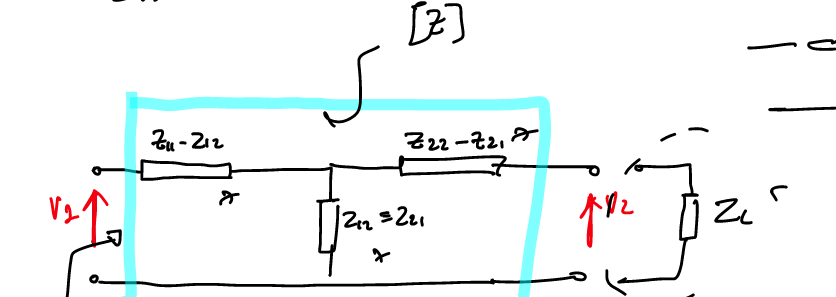
\includegraphics[scale=0.5]{immagini/rete_t_equiv.png}
		\caption{Rete "a T" equivalente alla rete a due porte}
	\end{figure}
	\\\\calcolando l'impedenza in ingresso $Z_{in}^{(1)}$ corrisponde a quella di una rete a due porte.\\Si può fare risolvendo il circuito (che viene lasciato per esercizio?) ottenendo 
	\begin{equation}
	Z_{in}^{(1)} = Z_{11} - \dfrac{Z_{12}^2}{Z_{22} - Z_L}	
	\end{equation}
	\\Se nell'antenna da sola bastava la Z in ingresso qui serve la matrice Z, e questo si chiama impedenza passiva, tiene conto dell'altro oggetto ma non alimentato (se fosse alimentato ci vorrebbe l'impedenza attiva e sarebbe più complesso).
\end{itemize}
Vogliamo esprimere la potenza che viene raccolta dal carico del rx rispetto a quella che viene mandata in ingresso ed (altro) ed introdurremmo il guadagno di trasduzione.\\Ripartiamo dalla rete a due porte, che rappresentiamo con la matrice di impedenza\\
\begin{figure}
	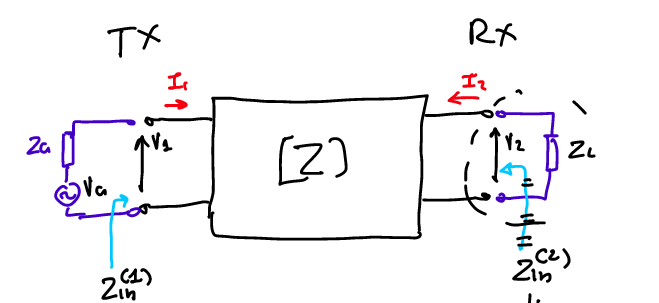
\includegraphics[scale=0.5]{immagini/rete_dp_matr.png}
	\caption{Rete a due porte con matrice d'impedenza}
\end{figure}
\\\\possiamo quindi vedere le impedenze in ingresso alle diverse porte del tx e dell'rx, sappiamo che sono date da:
\begin{equation}
	Z_{11}^{(1)} = Z_{11} - \frac{Z_{12}^2}{Z_{22}+Z_L}	
\end{equation}
e 
\begin{equation}
	Z_{22}^{(2)} = Z_{11} - \frac{Z_{12}^2}{Z_{11}+Z_G}	
\end{equation}
Vediamo l'equivalenza di Thevenhin:\\
\begin{figure}
	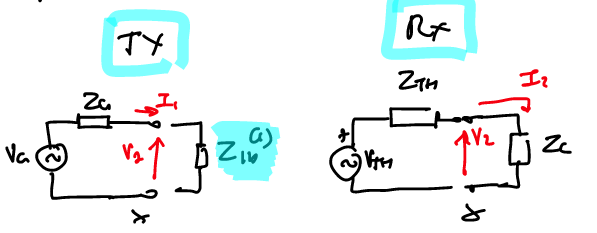
\includegraphics[scale=0.6]{immagini/equiv_thev_rx_tx.png}
	\caption{Equivalenza di Thevenhin per rx e tx}
\end{figure}
\\\\guardando da sinistra, un'osservatore vedrà tutto quello che accade dentro dal valore di $Z_{11}^{(1)}$ e questo è per il tx, mentre per l'rx: ci saranno impedenza di Thevenhin e generatore di Thevenhin che vanno calcolate.\\Possiamo quindi studiarli separatamente, nel secondo valuteremo la potenza che verrà distribuita sul carico.\\Partiamo dalla $Z_{Th}$ che è l'impedenza passiva che vediamo verso l'interno avendo staccato il generatore, quindi è uguale all'impedenza di ingresso che avremmo calcolato con il circuito attivo 
\begin{equation}
	Z_{Th} = Z_{in}^{(2)}	
\end{equation}
\\La tensione del generatore è data dal fatto che il circuito è aperto, riprendiamo l'espressione di $V_2$ circuitale 
\begin{equation}
	V_2 = Z_{21}I_1	
\end{equation}
in quanto il termine con $I_2$ È 0 perché i circuiti sono staccati.\\Esplicitiamo
\begin{equation}
	V_1 = V_{C1} - Z_G I_1 \equiv Z_{11}I_1 + Z_{12}I_2\bigg\rvert_{I_2 = 0}
\end{equation}
sapendo che $I_2$ = 0 avremo 
\begin{equation}
	I_1 = \dfrac{Z_G}{Z_{11} + Z_G}	
\end{equation}
Inseriamo l'espressione trovata per trovare la 
\begin{equation}
	V_{Th} = V_2 = \dfrac{Z_{21}}{Z_{11} + Z_G} V_G	
\end{equation}
Ora possiamo usare i due circuiti per fare delle considerazioni di potenza: consideriamo 2 potenze
\begin{itemize}
	\item $P_L$, che il trasmettitore rilascia al carico del ricevitore.\\È data da 
	\begin{equation}
		P_L = \frac{1}{2} R_{L}|I_2|^2	
	\end{equation}
	è quella che serve al dispositivo impiantato per farlo funzionare. La $I_2$ si ricava da
	\begin{equation}
	I_2 = \dfrac{V_{Th}}{Z_{in} + Z_L}	
	\end{equation}
	quindi
	\begin{equation}
		P_L = 
		\frac{1}{2} \dfrac{\abs{Z_{21}}^2 \abs{V_G}^2 R_L}{\abs{Z_{11} + Z_G}^2} \dfrac{1}{\abs{Z_{22} - \frac{(Z_{21}^2)}{Z_{11 + Z_G}} + Z_L}^2}
		= \frac{1}{2} \dfrac{\abs{Z_{12}}^2 \abs{V_G}^2 R_L}{\abs{(Z_{11} + Z_G)(Z_{22}+Z_L) - Z_{12}^2}^2}
	\end{equation}
	\item $P_{in}^{(1)}$ che è quella che entra nell'antenna trasmittente data da 
	\begin{equation}
		P_{in}^{(1)} = \frac{1}{2}R_{in}^{(1)} |I_1|^2 
	\end{equation}
	In particolare 
	\begin{equation}
		P_{in}^{(1)} = \frac{1}{2}R_{in}^{(1)} \dfrac{\abs{V_G}^2}{\abs{Z_{11} + Z_G}^2}
	\end{equation}
\end{itemize}
Definiamo ora la \textbf{potenza disponibile} in ingresso (available power) che è la $P_{AV,G}$ che è la massima potenza che il generatore può erogare verso la rete e che viene erogata nelle condizioni in cui l'impedenza delle rete è il complesso coniugato dell'impedenza del condensatore 
\begin{equation}
	Z_{in}^{(G)} = Z_G^*	
\end{equation}
(adattamento coniugato, $R_{in}^{(1)} = R_G$ e $X_{in}^{(1)} = -X_G$)
quindi 
\begin{equation}
	P_{AV,G} = \dfrac{\abs{V_G}^2}{8R_G}	
\end{equation}
Qualcosa del genere si fa in uscita ed è la \textbf{network available power}, che è la massima potenza che la rete è in grado di rilasciare al carico e si ha la massima quando l'impedenza in ingresso in 2 è uguale al complesso coniugato della $Z_L$.\\Vale 
\begin{equation}
	P_{AV,N} = max{PL} = \dfrac{\abs{V_{Thev}}^2}{8 R_{Th}}	
\end{equation}
Definiamo finalmente il $G_T$ (transducer power gain) uguale per definizione a
\begin{equation}
	G_T \triangleq \frac{P_L}{P_{AV,G}} 	
\end{equation}
ed è importantissima perché dipende dal fatto che rx non è adattato al carico, che c'è un mezzo con perdita etc... e la dobbiamo ottimizzare perché sappiamo che
\begin{equation}
	P_L = P_{AV,G} G_T	
\end{equation}
sostituendo nella precedente viene fuori la relazione
\begin{equation}
	G_T = \dfrac{4R_G R_L \abs{Z_{12}}}{\abs{ (Z_{11} + Z_G) (Z_{22} + Z_L) - Z_{12}^2}^2}
\end{equation} 
(che è adimensionale essendo un guadagno). (N.B: la X è la reattanza).È la grandezza da tenere in conto quando si progetta il sistema.


\chapter{Lezione 7}
\section{Ancora sul guadagno di trasduzione}
Possiamo scrivere la potenza che finisce sul carico $P_L$, che è quella che serve al dispositivo se non ha una batteria per accendersi come 
\begin{equation}
	P_L \equiv P_{R\rightarrow T} P_{AV,G} G_T	
\end{equation}
(il pedice T indica il transponder) dove $G_T$ è specifica della configurazione, quindi se ad esempio ruoto un dispositivo rispetto all'altro devo ricalcolare il guadagno di trasduzione.\\In ingegneria è solito calcolare il margine, che è \textsf{\textbf{ciò che permette di dormire la notte}}, ovvero avere della capacità in più per le evenienze: $p_0$ è la minima potenza da rilasciare sul carico tale per cui il ricevitore funzioni, ovvero la $min\{P_L\}$, il margine in scala lineare è 
\begin{equation}
	M = \frac{P_L}{p_0}	
\end{equation}
dove $p_0$ è la power sensitivity.\\Se la quantità è $<$ 1 stiamo rilasciando una potenza più piccola di quella che serve al dispositivo per funzionare, quindi non avremo il link, mentre più è maggiore di 1 e più il link è robusto.\\Normalmente si rappresenta in DB: 
\begin{equation}
	M_{db} = P_{AV,G} + G_T -p_0 - M_0	
\end{equation}
dove $M_0$ è un margine aggiuntivo che cerca di tenere conto di eventuali difetti fisici dell'oggetto per cui conta che viene mantenuta della potenza in più.\\Il radio collegamento si stabilisce quando $M_{db} > 0$, quindi più è grande più si compensano fenomeni di cui non si era tenuto conto durante il progetto.\\\textbf{Con margine pari a 0 ce dice bene se funziona na volta sola a culo}, mentre invece con della potenza di riserva c'è una sicurezza maggiore.\\esempio:\\ 
\begin{figure}[!h]
	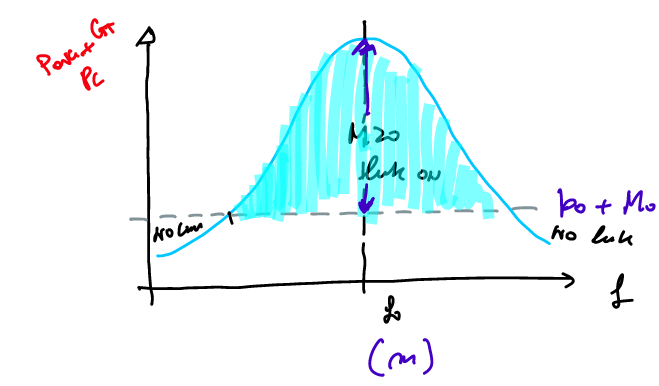
\includegraphics[scale=0.5]{immagini/margine_sens.png}
\end{figure}\\\\
la linea rappresenta la sensitivity + margine aggiuntivo, quindi dire che $M_{db} > 0$ vuol dire che $P_{AV,G} + G_T > p_0 + M_0$. Se abbiamo progettato bene il dispositivo il picco sarà sulla frequenza di lavoro $f_0$, avremo quindi una regione dove c'è il collegamento ed una dove non c'è.\\Il grafico si fa spesso rispetto anche ad un parametro di progetto, come ad esempio la dimensione, la freccia viola indica quanto si è sicuri che il dispositivo sia robusto rispetto a delle cose che non si è riusciti a prevedere.\\Fissata la potenza in ingresso (che è strettamente finita) occorre progettare i dispositivi al meglio possibile in modo che $G_T$ sia elevato.

\subsection{Guadagno di sistema}
(Orfanidis, pdf free: libro di EM dove nel cp 5 c'è questa parte).\\Il guadagno di sistema è definito come:
\begin{equation}
	g = \dfrac{\text{max}\{P_L\}}{\text{Potenza entrante nella rete} (P_in)} = \frac{P_{av,in}}{P_{in}}
\end{equation}
dove la massima $P_L$ è quella che abbiamo chiamato la $P_{av,in}$.\\Questa espressione differisce da quella di prima in quanto presuppone l'adattamento coniugato in ingresso ed in uscita, quindi è il caso migliore: se il transponder venisse progettato perfettamente adattato rispetto a ciò che vede in ingresso e l'interrogatore perfetto rispetto a ciò che arriva dall'esterno avrei questo massimo: per l'adattamento coniugato deve valere:
\begin{itemize}
	\item $Z_{in}^{(1)} = Z_{G}^*$
	\item $Z_{in}^{(2)} = Z_{L}^*$
\end{itemize}
moltiplicando: 
\begin{equation}
	g \cdot P_{in} = P_{L,max}
\end{equation}
otteniamo l'upper bound per il link.\\ \textbf{Perché è importante:} quando si fa un progetto, non si "spacca subito il capello" se magari ci sono molti parametri, quindi se il link va progettato secondo certe condizioni ci si chiede se occorre progettare l'antenna proprio così.\\Posso assicurare che le due antenne riescano a comunicare? Quello che si fa è fare un design di massima senza preoccuparsi di adattare subito le antenne, ma messe in un certo modo nel caso migliore si riesce a tx una potenza sufficiente da poter fare accendere l'antenna rx? Allora controllo il guadagno di sistema, se mi ci trovo e quindi il margine è sufficiente per lavorare, allora penso a poter ottimizzare le antenne per poter lavorare.\\Il calcolo si ottiene mettendo le espressione trovate prima:
\begin{equation}
	g = \dfrac{\frac{1}{8}\frac{\abs{V_{Th}}^2}{R_{Th}}}{\frac{1}{2} \dfrac{\abs{Z_{12}}^2 R_L \abs{V_G}^2}{\abs{(Z_{11}+Z_G)(Z_{22}+Z_L) - Z_{12}^2}^2}}
\end{equation}
Esiste poi un'espressione molto pulita se si fa riferimento alla \textbf{matrice di scattering}, "cugina" della matrice di impedenza, ovvero è una rappresentazione con un'onda di tensione che entra che è $a_1$ ed un'onda di tensione che torna indietro (l'onda riflessa dall'interfaccia) $b_1$ ed anche le $a_2, a_2$ dove $V_1$ e $V_2$ in funzione di A:
\begin{equation}
	V_1 = \sqrt{Z_0}(a_1 + b_1)
\end{equation}
\begin{equation}
	V_2 = \sqrt{Z_0}(a_2 + b_2)
\end{equation}
si può anche trovare una relazione matriciale, ($Z_0$ è l'impedenza di riferimento della linea. Tipicamente, se il carico non è complesso, sono 50$\Omega$) e la matrice di scattering è tale per cui:\\ 
\begin{equation}
	\begin{bmatrix}
		b_1\\
		b_2
	\end{bmatrix} = 
	\begin{bmatrix}
		S_{11} & S_{12}\\
		S{21} & S_{22}\\
	\end{bmatrix} \cdot
	\begin{bmatrix}
		a_1\\
		a_2
	\end{bmatrix}
\end{equation}
per capirci l'$S_{11}$ corrisponde al coefficiente di riflessione della porta 1 isolata dalla 2.\\Otteniamo quindi un'espressione del guadagno di sistema: 
\begin{equation}
	g = \dfrac{\abs{S_21}^2}{(1-\abs{S_{11}}^2)(1 - \abs{S_{22}}^2)}
\end{equation}
\textbf{Esempio:}\\
immaginiamo di avere un moncherino di un braccio, nel quale siano stati impiantanti dei sensori miografici che raccolgono gli impulsi della mano che si apre/chiude (\textbf{perché il muscolo lo ricorda :O}). Immaginiamo di mettere due sensori A e B e sopra l'antenna TX\\
\begin{figure}[!h]
	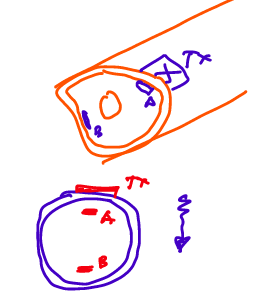
\includegraphics[scale=0.5]{immagini/moncherino.png}
	\caption{Sensori su moncherino (la seconda immagine è la vista in sezione)}
\end{figure}
\\\\si usano due sensori perché si acquisisce il segnale del muscolo agonista ed antagonista. I due dispositivi sono a differenti profondità rispetto al TX e quindi daranno guadagni di trasduzione diversi.\\Immaginiamo di aver calcolato i guadagni di trasduzione, troviamo questa situazione:
\begin{table}
	\begin{tabular}{|c|c}
		 & G[DB]\\
		 \hline
		 A & -15\\
		 B & -25\\
	\end{tabular}
\end{table}
$p_0 = -15 dBm$, dove x dbM = xdB - 30, quindi se 1W = 0dB $\rightarrow$ 1W = 30dbM (1W = 1000 mW)\\$M_0 = 3dB$, cerchiamo la $P_{av,G}$ per attivare il link fra i due dispositivi.\\Abbiamo visto che $P_{av,G} + G_T > p_0 + M_0$, $P_{av,G} > -G_T + p_0 + M_0$. Riconduciamo alla stessa unità di misura poi:
\begin{itemize}
	\item[A] $P_{av,G} = -15dBm + 3dB + 15dB$. Portiamo tutto in dBm, riscriviamo $P_{av,G} = M_0\frac{p_0}{G_T}$, vanno espressi $p_0$ e $G_T$ o in W o in mW. Quindi, in dB: -45dB +3dB +15dB = -27dB, che sono 3dBm ovvero 2mW.
	\item[B] +25dB -15 dbM +3dB.\\Riportiamo tutto in dB, +25dB (-15-30)dB + 3dB = -17 dB. Conviene riportare tutto in DB visto che il margine aggiuntivo è espresso in dB.
\end{itemize}
\textbf{tenere presente che:}
\begin{itemize}
	\item 3dB $\approx$ 2W e quindi per i dBm si ragiona in mW.
\end{itemize}

\subsection{Link asimmetrico - guadagno di Round-Trip}
Consideriamo di avere un ricevitore RX che sia privo di sorgente e per comunicare con il trasmettitore deve usare la modulazione del segnale di interrogazione (simile a ciò che avviene nei link induttivi).\\Prendiamo il circuito di Thevenhin del RX:\\
\begin{figure}
	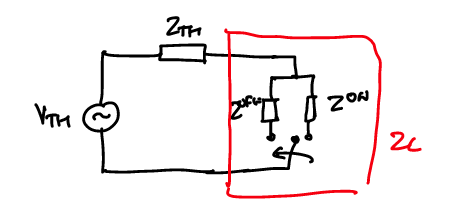
\includegraphics[scale=0.5]{immagini/thev_rx.png}
	\caption{Circuito di Thevenhin del ricevitore senza sorgente}
\end{figure}
\\\\immaginiamo che nella modalità in cui $TX \rightarrow RX$ il carico venga collegato ad uno switch che in base ad una logica binaria, se si vuole trasmettere 1 o 0, commuta su uno dei due carichi.\\I due carichi sono molto diversi, quindi normalmente $Z^{OFF} >>> Z^{ON}$.\\I due dispositivi sono accoppiati, quindi il trasmettitore si accorgerà che dall'altra parte sta cambiando qualcosa:\\
\begin{figure}
	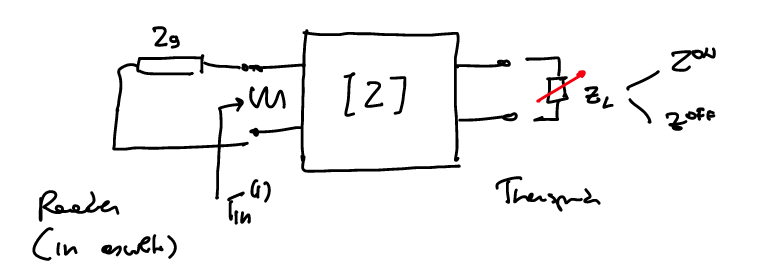
\includegraphics[scale=0.5]{immagini/rete_dp_2.png}
	\caption{Schema della rete a due porte}
\end{figure}
\\\\Il coefficiente di riflessione che il reader vede è dato da
\begin{equation}
	\Gamma^{(1)} = \frac{Z_{in}^{(1)} - Z_g}{Z_{in}^{(1)} + Z_g}
\end{equation}
l'impedenza tramite $Z_in^{(1)}$ è funzione del particolare stato di commutazione del carico.\\Si può far vedere che ci sono segnali sinusoidali che vengono trasmessi, rimuovendo la portante si vede che la potenza che il transponder manda indietro al reader si scrive come
\begin{equation}
	P_{R \leftarrow T} = \frac{1}{4} \abs{\Gamma_{in}^{(1)} (Z^{ON}) - \Gamma_{in}^{(1)}(Z^{OFF})}^2 \cdot P_{av,G}
\end{equation}
quindi dipende dalla potenza massima iniettata nella porta moltiplicata per una grandezza che dipende dai valori di impedenza.\\Valori tipici:
$Z^{OFF} \rightarrow \infty$
$Z^{ON} \rightarrow Z_L$.\\Quindi come caratterizziamo il link andata e ritorno: introduciamo il guadagno di Round-Trip definito come:
\begin{equation}
	G_{RT} = \frac{P{R \leftarrow T}}{P_{a, G}} = \frac{1}{4} [\Gamma_{in}^{(1)} (Z^{ON}) - \Gamma_{in}^{(1)}(Z^{OFF})]^2
\end{equation}
che è data da 
\begin{equation}
	\abs{\dfrac{Z_G \cdot Z_{12}^2}{Z_{11} + Z_G}}^2 \cdot \dfrac{1}{\abs{(Z_{11}+Z_G)(Z_{22}+Z_L) - Z_{12}^2}^2}
\end{equation}
dove deve valere la condizione:
\begin{equation}
	P_{R \leftarrow T} = P_{av,G}G_{RT} > p_R
\end{equation}
per stabilire il link totale inverso.\\Possiamo anche qui definire un margine di Round-Trip (in dB siamo in scala 10$log_{10}$):
\begin{equation}
	M_{RT}\bigg{\rvert{dB}} = P_{av,G} + G_{RT} - p_R - M_0
\end{equation}
quando la quantità è $\geq 10$ abbiamo che il link inverso è attivato.\\
\begin{figure}[!h]
	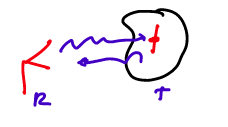
\includegraphics[scale=0.5]{immagini/read_trans.png}
\end{figure}\\\\
c'è il segnale che va dal reader al transponder e poi dal transponder torna indietro e viene raccolto dal reader. Abbiamo quindi due margini:
\begin{itemize}
	\item per il link diretto:
	\begin{equation}
		M_D = P_{av,G} + G_T - p_T - M_0
	\end{equation}
	\item per il link di Round-Trip:
	\begin{equation}
		M_{RT} = P_{av,G} + G_T - p_T - M_0
	\end{equation}
\end{itemize}
quindi il link è stabilito quando ambe due le grandezze sono maggiori di 0, altrimenti può accadere che accendo il transponder ma questo risponde "debolmente" o viceversa.\\Tipicamente qui il bottleneck è l'$M_D$ perché tipicamente la sensitivity del transponder è molto più "scarsa", specialmente se questo è senza batteria.\\Se il link diretto è verificato ho quindi buone possibilità che lo sia anche quello inverso (ma non è sempre così).\\\\In generale, $G_{RT} << G_T$ perché nel primo caso c'è un'attenuazione dovuta al fatto che entra e poi torna indietro quindi se il mezzo è con perdite subisce due forti attuazioni invece di una sola.\\\\La maggior parte di questi link funziona posizionando il lettore sul corpo e leggendo dal dispositivo impiantato. Ci sono dei casi in cui c'è vantaggio a leggere il dato da fuori, ad esempio protesi che monitorano le infezioni in modo che ad esempio un lettore che è in bagno legga il dato per individuare i precursori dell'infezione.\\Ovviamente si è esposti ad attacchi malevoli.

\section{Link in campo lontano}
Qui valgono tutte le grandezze inserite studiando le antenne classiche. Questo tipo di link si ha tipicamente quando abbiamo dispositivi wearable che comunicano con l'esterno:\\
\begin{figure}[!h]
	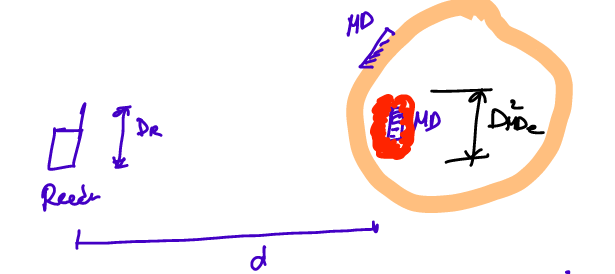
\includegraphics[scale=0.5]{immagini/com_far_field.png}
	\caption{Esempio di link di comunicazione in far field}
\end{figure}\\\\
abbiamo il corpo ed immaginiamo che il dispositivo sia o all'esterno o anche all'interno ma venga interrogato a distanza.\\Abbiamo il reader (interrogatore) e la distanza $d$ è tale per cui ogni oggetto è nel campo lontano dell'altro, da cui la \textbf{distanza di Fraunhofer}:
\begin{equation}
	r_F \geq \frac{2D^2}{lambda}	
\end{equation}
Per il reader, abbiamo
\begin{equation}
	d > \frac{D_r^2}{\lambda}	
\end{equation}
dove $\lambda_0$ è sempre quello nel vuoto.\\Per il dispositivo sul corpo, la dimensione che conta è quella dove c'è della distribuzione di corrente ovvero dove il corpo diventa un pezzo dell'antenna e quindi 
\begin{equation}
	d > \frac{D_{MD}^2}{\lambda_0}
\end{equation}
dove immaginiamo una zona dove ci sono delle correnti di conduzione che possono a loro volta produrre delle radiazioni.\\In queste condizioni, possiamo studiare i due oggetti separatamente per poi metterli assieme con le regole di campo lontano:\\
\begin{figure}[!h]
	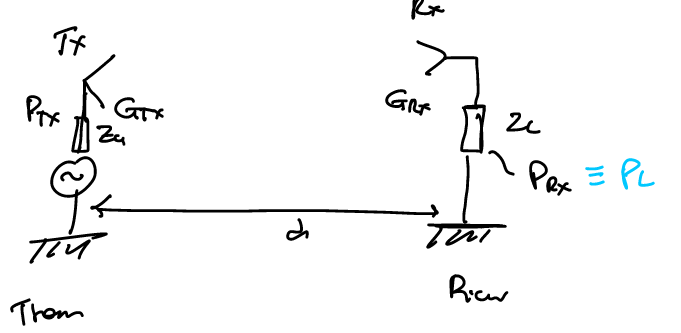
\includegraphics[scale=0.3]{immagini/tx_rx_far.png}
\end{figure}\\\\
il trasmettitore sarà caratterizzato da guadagno e potenza entrante mentre il ricevitore dal guadagno e dalla potenza rilasciata sul carico, allora (Friis)
\begin{equation}
	P_{RX} = P_{TX} G_{TX} G_{RX} \tau_{TX} \tau_{RX} (\frac{\lambda4\pi d})^2 \eta_p
\end{equation}
dove abbiamo:
\begin{itemize}
	\item $\tau_{TX}$ vale 
	\begin{equation}
		\tau_{TX} = 4\pi \dfrac{R_{TX} R_G}{\abs{Z_{TX} + Z_G}^2}
	\end{equation}
	mentre $\tau{RX}$
	\begin{equation}
		\tau_{RX} = 4\pi \dfrac{R_{RX} R_L}{\abs{Z_{RX} + Z_L}^2}
	\end{equation}
	e valgono 1 quando c'è adattamento coniugato: 
	\[
	\begin{cases}
		\tau_{TX} = 1 & \text{se} Z_{TX} = Z_G^*\\
		\tau_{RX} = 1 & \text{se} Z_{RX} = Z_L^*
	\end{cases}
	\]
	
	\item I prodotti sono il guadagno realizzato di TX ed RX 
	\begin{equation}
		G_{TX} \cdot \tau_{TX} = \tilde{G}_{TX}
	\end{equation}
	\begin{equation}
		G_{RX} \cdot \tau_{RX} = \tilde{G}_{RX}
	\end{equation}
	(rx tiene conto del fatto che non tutta la potenza raccolta può essere trasferita al carico perché può esserci del disallineamento).
	
	\item La $\eta_P$ tiene conto di come sono allineate la polarizzazioni fra le due antenne (efficienza di polarizzazione), matematicamente: 
	\begin{equation}
		\eta_P = \abs{\underline{\hat{h}}_{RX} \cdot \underline{\hat{h}}_{TX}}^2
	\end{equation}
	
	\item Il termine $(\frac{\lambda_0}{4 \pi d})^2$ è l'attenuazione di spazio libero, quindi la densità di potenza si attenua per volumi più grandi in quanto si distribuisce man mano che ci allontaniamo su sfere più grandi.\\Il $^2$ vale solo per lo spazio libero, altrimenti ci sarà un valore più altro se ci sono riflessioni da terreno pareti etc...
\end{itemize}


\chapter{Lezione 8}
\section{Far field - link simmetrici}
Abbiamo considerato il link diretto, dove abbiamo che i due dispositivi sono posti a distanza grande rispetto alla distanza di Fraunhofer.\\Continuiamo con link diretti, ricaviamo dalla formula di Friis la distanza massima del collegamento: introduciamo una p del ricevitore che è la power sensitivity del ricevitore: se $P_{rx} \geq p_{rx}$ allora li link sarà attivo altrimenti non si stabilisce.\\Considerando l'uguaglianza, $P_{rx} = p_{rx}$, possiamo trovare la distanza massima per cui tale collegamento si stabilisce: facciamo Friis$^{-1}$ e troviamo che
\begin{equation}
	d_{max} = \frac{\lambda}{4\pi} \sqrt{\dfrac{G_{TX} P_{TX}G_{RX}\tau_{TX} \tau_{RX}}{p_{rx}} \eta_P}	
\end{equation}
dove:
\begin{itemize}
	\item se il tx è adattato, abbiamo una proporzionalità $\propto \sqrt{\frac{G_{RX}}{p_{RX}}}$
	\item se invece c'è adattamento anche con il ricevitore c'è proporzionalità con  $\propto \sqrt{G_{RX}}$
\end{itemize}
In dB, avremo che 
\begin{equation}
	d_{max}\bigg\rvert_{dB} \propto \frac{1}{2} G_{RX}\bigg\rvert_{dB}
\end{equation}
sappiamo che 3dB è circa un 2x di guadagno, ogni 6dB (4 volte di guadagno) si ha un raddoppio della distanza del link (la radice la porta a 2).\\Invece, un aumento di guadagno di 3dB dice che la distanza di lettura aumenta di un fattore $\sqrt{2}$ (circa 1 volta e mezza) (IMPORTANTE).\\Facciamo un grafico per questo concetto:\\
\begin{figure}[!h]
	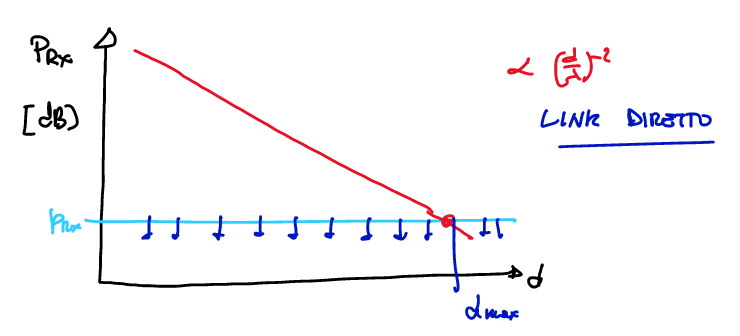
\includegraphics[scale=0.4]{immagini/gain_dist.png}
\end{figure}\\\\
c'è un'attenuazione che andrebbe come $(\frac{d}{\lambda})^{-2}$. Avendo quindi fissato il sistema di lettura, un modo per aumentare la distanza è cercare di abbassare la sensitivity (ma ci sono i limiti fisici ad un certo punto).\\Per link simmetrici vale la stessa cosa, basta invertire rx con tx, in questo caso il trasponder è dotato di una sorgente locale di alimentazione.

\section{Far field - link asimmetrici}
Qui i ruoli fra transponder ed interrogatore non si scambiano mai, applicheremo quindi nuovamente un protocollo di modulazione dell'impedenza, ma non nell'accoppiamento bensì nel back scattering (riflessione).\\Immaginiamo la seguente situazione:\\
\begin{figure}[!h]
	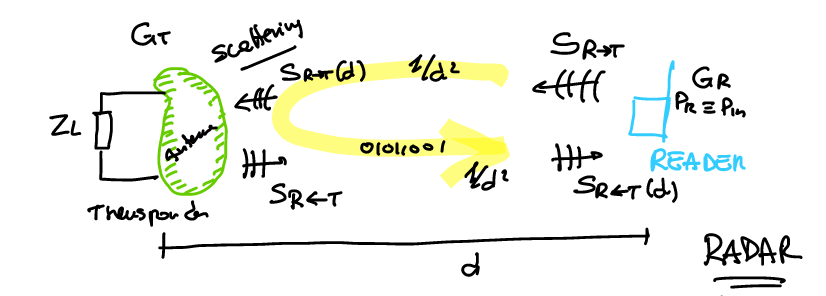
\includegraphics[scale=0.4]{immagini/back_scatt.png}
\end{figure}
\\\\la distanza d è di campo lontano, il reader avrà un suo guadagno $G_R$ ed anche il transponder $G_T$.\\Il reader manderà un segnale ed il transponder lo andrà a riflettere modulandolo: avremo un vettore di Pointing dal transponder verso il reader e poi ci sarà un giro di round trip indietro, abbiamo un fenomeno di \textbf{scattering}, che verrà pilotata dal carico.\\Questo è il classico modello radar, dove c'è un antenna che manda impulsi verso un aereo ma qui la differenza è che il segnale che torna indietro deve portare informazione ovvero una sequenza binaria.\\Scriviamo la densità di potenza 
\begin{equation}
	S_{R \rightarrow T}(d) = \frac{1}{2Z_0}\abs{E_{R \rightarrow T}(d)}^2	
\end{equation}
che si può anche scrivere come 
\begin{equation}
	S_{R \rightarrow T}(d) = I_{R \rightarrow T} \cdot \frac{1}{d^2}
\end{equation}
dove la I è l'intensità di radiazione che è densità di potenza per unità di angolo solido ($\frac{W}{sk}$).\\Entra in gioco nel guadagno dell'antenna trasmittente
\begin{equation}
	G_R = \frac{I_R 4\pi}{P_R}	
\end{equation}
da cui possiamo ricavare 
\begin{equation}
	P_R = \frac{P_{in}G_R}{4 \pi}	
\end{equation}
la inseriamo nell'espressione della densità di potenza ottenendo 
\begin{equation}
	S_{R \rightarrow T}(d) = \frac{P_{in}G_R}{4 \pi d^2}	
\end{equation}
che ci dice come si attenua la potenza man mano che ci si allontana da una sfera di raggio d.\\Introduciamo ora il concetto di \textbf{radar cross-section}: è l'area di uno scatteratore isotropico (riflette allo stesso modo in tutte le direzioni), quindi una sferetta metallica, che una volta investita dal campo retro-diffonde nella direzione dove c'è il mio oggetto la stessa quantità di potenza.\\È la $\sigma$, che va valutata in campo lontano ($d \rightarrow \infty$):
\begin{equation}
	\sigma = \lim\limits_{r \rightarrow \infty} 4 \pi r^2 \dfrac{S^{scatt}}{S^{in}} = \lim\limits_{r \rightarrow \infty} 4 \pi r^2 \dfrac{\abs{E^{scatt}}^2}{\abs{E^{in}}^2}
\end{equation}
Come si utilizza: conosciamo il campo incidente, possiamo quindi calcolare il campo che emerge dal transponder e torna indietro dal ricevitore: 
\begin{equation}
	S_{R \leftarrow T}(d) = \sigma \dfrac{S_{R \rightarrow T}(d)}{4\pi d^2}
\end{equation}
è la potenza $S_{R \leftarrow T}(d)$ e che quindi porterà il segnale che torna indietro.\\La potenza rilasciata sul carico del ricevitore sarà uguale a: 
\begin{equation}
	P_{R \leftarrow T}S_{R \leftarrow T}(d) \cdot A_{C,R}
\end{equation}
dove $A_C$ è l'area efficace del reader, ovvero una superficie equivalente che se investita da un'onda raccoglie una quantità di potenza uguale da quella che avrebbe raccolto l'antenna (ed è più piccola dell'area geometrica): 
\begin{equation}
	A_e = \lambda^2 \frac{G}{4 \pi}
\end{equation}
Mettendo quindi tutto dentro: 
\begin{equation}
	P_{R \leftarrow T} = \dfrac{P_{in}G_RA_{e,R}}{(4\pi d^2)^2} \eta_P \sigma_T
\end{equation}
ci aggiungiamo $\eta_P$, che è il \textbf{polarization loss factor}, perché se abbiamo un oggetto di una certa forma ed irradiamo con un campo, per effetto della forma probabilmente il campo scatterato avrà una forma differente, quindi quando incide sull'antenna può non avere la stessa polarizzazione di quando è partito e quindi si tiene in conto con questo fattore.\\Questa è l'equazione del radar, dipende anche dalla capacità di scatterare del transponder in una direzione rispetto che in un'altra.\\Abbiamo anche che $\sigma$ può essere considerata in due casi:
\begin{itemize}
	\item monostatica: il segnale è raccolto dalla stessa antenna che interroga
	\item bistatico: abbiamo due antenne, una illumina il bersaglio ed un'altra prende il segnale retro-diffuso (tipicamente c'è un vantaggio per quanto riguarda la qualità del segnale)
\end{itemize}
ragioniamo con situazione monostatica:\\la potenza che torna indietro è $\propto \frac{1}{d^4}$ perché deve fare un round trip quindi abbiamo due attenuazioni da $\frac{1}{d^2}$ quindi il segnale retrodiffuso è molto flebile rispetto ad un oggetto che sta trasmettendo di suo.\\Dobbiamo ora fare in modo che arrivi dell'informazione: occorre intanto isolare il dispositivo da tutto il riflesso dell'ambiente. Questo si ottiene con la modulazione, in modo che il segnale che si sovrappone al disturbo oscilli.\\Passiamo ad un'antenna che abbia un'impedenza d'ingresso $Z_a$ ed un carico $Z_L$ con un generatore equivalente che tiene conto del campo che arriva, possiamo esprimere $\sigma$ come
\begin{equation}
	\sigma = \frac{\lambda^2}{4 \pi} G \abs{A - \Gamma^*}^2 
\end{equation}
quindi è lo scattering di un dispositivo caricato.\\$\Gamma^*$ è un coefficiente di riflessione generalizzato, dato dal coefficiente che vedo fra l'antenna ricevente ed il suo carico. Ha come differenza rispetto al classico che c'è un complesso coniugato, perché c'è qualcosa che deve immagazzinare energia.\\ A è un complesso che dipende da forma e soprattutto dimensione dell'antenna scatterante: se la dimensione di tale antenna è $L << \lambda$ allora $A \simeq 1$. In queste condizioni la $\sigma$ del transponder sarà data da:
\begin{equation}
	\sigma_T = \frac{\lambda^2}{4\pi}G_T^2 \abs{1 - \dfrac{Z_L - Z_{in,T}^*}{Z_L + Z_{in,T}}^2}
\end{equation}
da cui, avendo $Z_{in,T} = Z_A$ e sviluppando il comun denominatore:
\begin{equation}
	\abs{\dfrac{Z_L + Z_{in,T}-Z_L +Z_{in,L}^*}{Z_L + Z_{in,T}}^2} = \dfrac{4R_{in,T}^2}{\abs{Z_L + Z_{in,T}}^2}
\end{equation}
ottenendo infine
\begin{equation}
	\sigma_T = \frac{\lambda^2}{4 \pi} G_T^2 \dfrac{4R_{in,T}^2}{\abs{Z_L + Z_{in,T}}^2} \eta_P 
\end{equation}
aggiungiamo di nuovo l'efficienza di polarizzazione perché l'oggetto può cambiare la polarizzazione.\\Questa è quindi l'area di scattering equivalente con un guadagno $G_T$ ed una certa impedenza del carico ($Z_L$), che  quella che possiamo variare per far variare l'RCS: possiamo quindi controllare quanto questo oggetto rifletta, se lo facciamo on due stati cambia l'informazione che torna indietro e quindi possiamo mandare informazione.\\Abbiamo che
\begin{equation}
	P_{R \leftarrow T} = (\frac{\lambda}{4 \pi d})^4 P_{in} G_R^2 G_T^2 \dfrac{4 R_{in,T}^2}{\abs{Z_L + Z_{in,T}}^2} \eta_P^2	
\end{equation} 
ci interessa che l'equazione sia dominabile andando ad agire sull'impedenza del carico.

\subsubsection{Modulazione di impedenza}
Immaginiamo di avere due stati:
\begin{itemize}
	\item 0, associato ad un'impedenza di carico che sia virtualmente un circuito aperto $Z_L \rightarrow \infty$, e quindi $P_{R \rightarrow T} = 0$
	\item per lo stato 1 si può scegliere: $Z_L = 0$ (corto circuito) che ci da una potenza 
	\begin{equation}
		P_{R \leftarrow T} = (\frac{\lambda}{4 \pi d})^4 P_{in}G_R^2G_T^2 \cdot \dfrac{4 R_{in,T}^2}{\abs{Z_{in,T}}^2} \eta_P^2 \neq 0
	\end{equation}
\end{itemize}
così possiamo cambiare a piacimento la potenza retro diffusa.\\Una scelta di questi due livelli ha un grosso limite: l'oggetto comincia a riflettere ciò che arriva, ma se il RX switcha fra $\infty$ e 0, l'aspetto critico è che, funzionando solo con l'energia che arriva da lontano, non raccolgo quindi potenza: non c'è un carico collegato, quindi la corrente raccolta non può essere immagazzinata.\\Conviene quindi che uno dei due stati sia compresa fra $0$ ed $\infty$, quindi prendiamo $Z_L = Z_{IN,T}^*$ dove quindi in questo stato assorbe e immagazzina energia, mentre nell'altro caso no: 
\begin{equation}
	P_{R \leftarrow T} = (\frac{\lambda}{4 \pi d})^4 P_{in} G_R^2G_T^2\eta_P^2
\end{equation}
non c'è più dipendenza fra le impedenze. Quindi, nel caso 1 non abbiamo carica remota per il dispositivo, perché non è in grado di raccoglierla.\\Vediamo ora come avviene effettivamente la comunicazione: nello spazio possiamo avere persone, altri oggetti che saranno di dimensioni sicuramente più grandi di quelle di tx ed rx. Quando tx produce il suo campo, immaginiamo un'onda continua che si distribuisce in varie direzioni avremo una riflessione non modulata, quindi la stessa sinusoide con la stessa frequenza (attenuata) che finirà sull'rx e poi l'effetto prodotto dalla modulazione di impedenza:\\ 
\begin{figure}[!h]
	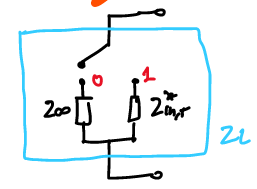
\includegraphics[scale=0.3]{immagini/mod_transp_01.png}
\end{figure}
\\\\abbiamo quindi nel carico del transponder nuovamente uno switch che connette due stati.\\Avremo quindi l'inviluppo con dentro l'onda che viene riflessa: ha la stessa frequenza del reader ma è modulata in ampiezza.\\Sul reader ci sarà la somma delle onde blu e rosse, l'ambiente grande rifletterà molto di più dell'oggetto che trasmette:\\
\begin{figure}[!h]
	\includegraphics[scale=0.3]{immagini/onda_verso_reader.png}
\end{figure}
\\\\ai capi del transponder vedremo quindi un qualcosa del genere:\\
\begin{figure}[!h]
	\includegraphics[scale=0.3]{immagini/ris_capi_transp.png}
\end{figure}
\\\\avremo quindi il segnale totale al reader, tolta la sinusoide rimane l'inviluppo e possiamo estrarre il valore inviato.\\Si chiama \textbf{modulazione di back scattering}, che è la tecnologia con cui funzionano tutti i sistemi di identificazione in radiofrequenza.\\Per la distanza massima del collegamento, dobbiamo tenere conto che 
\begin{itemize}
	\item il link diretto ($R \rightarrow T$),governato dalla formula di Friis serve ad accendere ed alimentare il transponder. Questo va come $(\frac{d}{\lambda})^2$ e si attiva quando $P_{R \rightarrow T} \geq P_T$
	\item il link inverso ($R \leftarrow T$), che va da transponder a reader e serve a modulare il backscattering. Va come $(\frac{d}{\lambda})^4$ Si attiva quando $P_{R \leftarrow T} \geq P_R$
\end{itemize}
il link si stabilisce quindi quando sono verificate ambe due le condizioni. Anche qui facciamo un grafico per capire la distanza massima del collegamento:\\
\begin{figure}[!h]
	\includegraphics[scale=0.2]{immagini/bs_max_d.png}
\end{figure}
\\\\ dove $p_R << p_T$ in quanto $p_R: -100dBm \% -70 dBm$ mentre $p_T: -20 dBm \% -5 dBm$, 

avremo quindi che $d_{max} = min\{d_D, d_I\}$ tipicamente il bottleneck è il link al quale compete la lunghezza più breve che è quasi sempre il link diretto.

\subsection{Logica di modulazione}
Cosa c'è nel transponder per acquisire energia e pilotare il transponder alto/basso: c'è una logica di modulazione che ha delle parti analogiche e delle parti digitali.\\Lo schema è il seguente:\\
\begin{figure}[!h]
	\includegraphics[scale=0.3]{immagini/log_mod.png}
\end{figure}\\\\
la prima cosa che avviene è un passaggio da analogico a digitale, c'è un rettificatore (immaginiamo un diodo collegato ad un condensatore, come se fosse la batteria virtuale del dispositivo) si passa quindi da AC a DC, la corrente alimenterà i componenti, primo fra cui il modulatore.\\Il modulatore comanda il carico e lo fa aprire o chiudere fra due valori, la frequenza a cui vengono fatte queste operazioni è tipicamente più bassa della $f_0$ di interrogazione: c'è un clock che scandisce tale frequenza, quindi anche il segnale di clock serve per gestire il modulatore. Abbiamo poi la RAM che mantiene l'informazione, da cui si legge e su cui si scrive.\\Tutta l'attività è svolta da un circuito integrato che è molto piccolo (chip da 0.5mm - 3mm)\\La prima parte è analogica dove avviene l'energy harvesting, ovvero il raccogliere l'energia, poi c'è il blocco di data modulation ed infine il data access che sono parti digitali.\\Il blocco analogico mette in contatto col mondo esterno, quello digitale serve per fare le operazioni.\\Da un punto di vista a radio frequenza, ci interessa la $Z_L$ per fare i calcoli di adattamento: vedremo l'impedenza del primo blocco analogico: avremo una parte reale dovuta alle perdite e poi un condensatore che serve ad immagazzinare l'energia che arriva da fuori, che può essere serie o parallelo\\
\begin{figure}[!h]
	\includegraphics[scale=0.3]{immagini/parte_imm.png}
\end{figure}\\\\avremo che $Z_C = R_{IC} - \frac{1}{j \omega C_{IC}}$ dove la parte $R_{IC}$ è tra $1 \Omega - 20 \Omega$, mentre il denominatore stra fra $100 - 200 \Omega$, è quindi questo il circuito a cui l'antenna di deve adattare per avere un $\tau_T = 1$, deve avvenire che\\ 
\[
	\begin{cases}
	R_{in,T} = R_{ic}\\
	X_{in,T} = -X_{in,C}	
	\end{cases}
\]
\\quindi l'antenna deve essere progettata per lavorare non in risonanza (induttanza ?), sarà l'insieme ad essere risonante.

\chapter{Lezione 9}
\section{Lezioncina di storia}
Abbiamo visto vari meccanismi di comunicazione sul corpo umano, sia a bassissima distanza con oggetti nel corpo, sia con oggetti sul corpo ed anche come possa avvenire la trasmissione di informazione senza usare batteria.\\Vediamo un implementazione di queste tecnologie di comunicazione basate su modulazione, introduciamo l'identificazione a radio frequenza: nata come evoluzione del codice a barre ed evoluta nelle applicazioni sensoristiche.\\Leon Theremin: inventore Russo dell'800, noto per il \textbf{theremin}: strumento musica suonato con le mani, sfrutta l'EM per suonare (ha un dipolo ed un loop), quindi muovendo le mani si può cambiare timbro ed altezza del suono.\\Guerra fredda: America e Russia non si vogliono bene ( :'( ), donarono all'ambasciatore Russo (?) un'antenna nascosta senza batterie, così che gli Americani avevano ascoltato le comunicazioni. Primo oggetto spia della storia inventato da Theremin, \textbf{the great seal bug}, la cosa interessante è che non aveva fonte di alimentazione: monopolo, che termina in una membrana sottile che è quindi una cavità risonante (un microfono a condensatore), le onde sonore mettevano in risonanza l'oggetto ma così non viene trasmesso nulla. Al di fuori, la spia inviava una portante a 300MHz, che viene raccolta dal monopolo. Questo vede una capacità variabile e gli cambia la frequenza di risonanza effettuando una modulazione in ampiezza (back scattering, 80 anni fa :O).\\\\È il primo esempio di dispositivo di spionaggio.\\Passati gli anni, venne ripreso per applicazioni civili

\section{IoT - introduzione}
La tecnologia dell'RFID si innesta nel contesto di come sta cambiando l'Internet adesso: l'Internet di ieri è una comunicazione host-to-host passando per la rete, oggi internet si sta "spalmando" nel mondo, quindi si mescola al tessuto quotidiano diventandone parte integrante.\\Già 30 anni fa si ipotizzava che il PC sarebbe stato spezzato e distribuito in casa su diversi schermi, senza più doversi sedere davanti al PC fisso.\\Quasi tutti gli oggetti oggi hanno delle espansioni digitali (es libri, QR code etc...), SPIME: (SPace + tIME), nell'internet di domani avremo un sistema nervoso che ingloba sia linee che trasmettono dati che nodi che includono sensori ed hanno capacità di captare cosa accade intorno.\\Tutti i sensori di mare, terra etc... servono per avere una comprensione maggiore per poter poi prendere delle decisioni in maniera più consapevole, il tutto è sia in macro-scala che micro-scala, ad esempio oggetti che possono essere impiantati nel corpo umano per capire meglio come questo funzioni.\\Arriviamo all'IoT, il presente: sensori apposti su qualunque tipo di oggetto nella manifattura dei dispositivi e comunicano con il nucleo di Internet mediante la comunicazione wireless.\\Ha molte declinazioni, fra cui "Industria 4.0", in cui non c'è solo il controllo automatico, la robotica ma anche l'interconnessione fra gli oggetti.\\Per avere IoT serve:
\begin{itemize}
	\item capacità di etichettare gli oggetti
	\item capacità di misurare una grandezza fisica
	\item la capacità di essere localizzato
\end{itemize}
es: il cellulare fa IoT, in quanto fra i compiti che svolge geolocalizza (AAAA GOOGLE SA DOVE SONO AIUTO), tracciando la posizione nel tempo: è possibile creare un "digital twin" del mondo reale, nel quale riusciamo a ricostruire anche le interazioni logiche e fisiche.\\Applicazioni dell'IoT: siamo ancora agli albori, si può immaginare di usare i dati in combinazione con AI per l'agricoltura di precisione (riducendo i pesticidi), smart cities, medicina smart etc... da qui viene estratta una "saggezza" ovvero la capacità di prendere decisioni.\\Il grosso degli oggetti interconnessi sono
\begin{itemize}
	\item automobili
	\item webcams
	\item ...
\end{itemize}
Noi (loro) siamo (sono) interessati in Internet of Helthcare Things: sono oggetti che possano essere identificati univocamente, connessi ad internet e capaci di comunicare l'un l'altro ed usati in ambiente medico. Cosa si può fare:
\begin{itemize}
	\item localizzare gli asset: in un ospedale ci sono molti oggetti, che si perdono. A livello minimo se ne fa il tracking
	\item gestione automatica delle risorse, dove in senso lato è anche capire lo stato di salute del paziente
\end{itemize}
Vantaggi:
\begin{enumerate}
	\item punto di vista del paziente: può essere monitorato in continuo da remoto, quindi poter avere la possibilità di avere warning nel caso in cui qualche parametro vitale stia andando fuori controllo (anche ad es. se si cade).\\C'è anche possibilità di avere assistenza da remoto in caso di eventi come cadute e non ultimo la possibilità di trasferire dati ad una centrale di controllo remota.\\Infine, consulti medici da remoto ed automatic reminder, ovvero la possibilità che la rete ricordi che devo fare delle cose come prendere delle medicine
	\item staff medico: un po' il duale, ovvero la possibilità di avere un accesso remoto allo storico del paziente.\\Poter usare algoritmi (AI) per individuare nei dati dei pattern anomali (pattern recognition?). Accesso alla cartella clinica del paziente con un web browser.
	\item manager: può meglio controllare il fatto che alcuni dispositivi vengano rubati, ma può anche avere una notifica quando questi escono da una certa area.\\Può fare analisi statistiche sul consumo di apparecchiature, ottimizzare il personale in una sala operatoria, capire come si muove il personale durante un intervento.\\Non ultimo, pianificare la manutenzione preventiva.
\end{enumerate}
Un oggetto è detto interconnesso quando ha una o più di queste caratteristiche:
\begin{itemize}
	\item identificazione
	\item localizzazione
	\item auto-diagnosi
	\item sensing
	\item attuazione (anche da remoto)
	\item local computing (edge computing: es, estrarre delle feature e mandare solo quelle nel cloud e non tutti i dati pesanti)
\end{itemize}
per interconnettere l'oggetto, si usa elettronica microscopica: oggetti piccoli quanto granelli di sabbia, che si collegano ad antenne di forma variabile in base alla frequenza, ottenendo una catena per cui c'è:
\begin{itemize}
	\item sensore, spesso senza batteria che contiene un ID e lo stato fisico di ciò che misura
	\item acceso da remoto con la tecnica di modulazione in back-scattering
	\item l'oggetto intermedio acquisisce l'informazione e lo manda nel cloud
\end{itemize}
È, a livello minimo, il \textbf{primo metro dell'IoT}, da cui si possono implementare tutti i servizi aggiuntivi.

\section{RFID}

In un sistema di identificazione ci sono:
\begin{itemize}
	\item identificatore che tx ed rx, dove ci sono aspetti di antenne, propagazione ed eventualmente sensistica
	\item transponder, spesso chiamato tag in quanto è nato come evoluzione del codice a barre. Riceve un comando, si attiva e rimanda un dato
\end{itemize}
ragioniamo su dispositivi di etichettatura EM: 
\begin{itemize}
	\item in principio ci sono state le etichette stampate, dove c'è tutto ciò che serve sapere e si legge
	\item codice a barre, salto concettuale enorme. È una rappresentazione visiva di un "numero" (\textbf{NUMERELLO SOTTO}). Rispetto al precedente, l'informazione non è scritta nel codice a barre, che appunto contiene solo un codice ed è quindi un puntatore ad un file dove c'è effettivamente l'informazione.\\Quindi si entra da tutt'altra parte dove poi si legge il dato: viene letto in maniera ottica, la distanza è di pochi cm (ma scandit ha fottuto questa distanza).
	\item carte magnetiche o smart card: funziona concettualmente come il codice a barre, ma mentre quest'ultimo è leggibile, qui è nascosto in un chip o codificato nella striscia magnetica quindi per leggerlo occorre dare energia dall'esterno. Possiamo quindi immagazzinare più dati, in alcuni casi riscriverli, ma senza adeguato lettore o software io, \textbf{UOMO DELLA STRADA} non posso leggere il dato
	\item RFID, dove il comportamento è lo stesso della smart card ma la lettura avviene in modalità wireless, quindi senza contatto galvanico.\\Anche qui c'è un puntatore e quindi il dato può essere cambiato senza cambiare il codice.
\end{itemize}
Differenza fra barcode ed RFID:
\begin{itemize}
	\item quantità di dati: in RFID c'è un microchip che può contenere fino a Kb di dati, barcode poche centinaia di bit
	\item RFID è difficile da leggere "in strada", barcode si
	\item se il barcode si riga o si incrosta non si legge, RFID è più tollerante
	\item se barcode è coperto manca di leggibilità ottica, RFID è meno sensibile
	\item copia o modifica non autorizzata: codice a barre si può copiare, RFID è difficile
	\item barcode si leggono uno alla volta, RFID si possono leggere "apparentemente" in più alla volta
	\item maggiore distanza di lettura di RFID (2m), cambia proprio la finalità del sistema
\end{itemize}
l'idea del transponder, prima di Theremin è nata durante la II WW, poi Theremin e nel 48' è uscito il primo articolo che descrive un sistema RFID completo.\\Già una decina di anni dopo ci sono anti-taccheggio (sistemi ad 1 bit senza elettronica).\\Avanzo dell'elettronica, per monitorare gli animali, anni 90' sistema molto noto è il Toll system (telepass) o l'immobilizer dell'automobile (es auto che non hanno chiavi).\\Nuovo secolo: inchiostri conduttivi, oggetti di tutti i tipi e chi più ne ha più ne metta.\\\\Funzionamento: un oggetto che include un microchiop ed un antenna e poi c'è un lettore: il lettore manda energia o comandi, il transponder raccoglie l'onda e rimanda un'informazione modulandola. Quando il tag passa sotto al lettore si stabilisce la comunicazione, non è necessaria la visibilità ottica fra reader e tag ed inoltre si possono leggere più tag alla volta.
\subsection{Classificazione}
Abbiamo 3 tipologie di tag e transponder:
\begin{itemize}
	\item attivi: hanno una fonte di alimentazione, tipicamente una batteria. Hanno a che fare tipicamente con i link simmetrici, possono trasmettere anche senza back scattering, hanno costi elevati ed autonomia scarsa, un esempio sono i tile (tracker BL) possono essere letti fino a 100aia di metri
	\item semi-passivi: tag a batteria ma non la usano per trasmettere ma solo per attività di bordo ovvero l'acquisizione del dato sensoristico che richiede poca energia mentre la comunicazione continua ad avvenire per riflessione. Serve anche per amplificare la capacità del chip, così che questo possa accendersi anche se la distanza è molta. Capacità elevata (ordine di anni, es il telepass: la batteria dura 4-5 anni), sono anche detti BAP (Battery Assisted Passive)
	\item passivi: il grosso che si trova, alimentati da remoto e funzionano solo con backscattering modulation. Costi anche più bassi di 5cent, distanze coperte minore di 20m.
\end{itemize}
Hanno campi di applicazione differenti: su una maglietta di Decathlon di mette un passivo, in un contenitore di vaccini di cui si vuole monitorare la temperatura si mette attivo o semi-passivo.\\SI può anche classificare in base alla memoria:
\begin{itemize}
	\item tag a bit unico: trasmettono un informazione binaria (ON/OFF) e sono usati come sistemi anti-taccheggio: c'è un "varco" formato da coil ed abbiamo il tag, funziona in due modalità:
	\begin{enumerate}
		\item sistema acusto-magnetico: ci sono due strisce di metallo vicine. La prima striscia è fatta di materiale ferro magnetico amorfo che quando eccitato da un campo magnetico ad opportuna frequenza oscilla (come una corda). tipicamente riceve toni a 58KHz, quindi oscillando va a modulare il campo EM. Il coil dell'anti-taccheggio si accorgerà quindi che c'è qualcosa. Di fianco c'è il secondo, che invece è un magnete, puù rigido del primo, che tende ad amplificare il campo magnetico prodotto dall'interrogatore. Ha un effetto di enfasi sulla risonanza della prima striscia, non è in contatto con la prima.\\La prima striscia serve a comunicare che c'è al varco, la seconda striscia fa si che, se deattivata, il disturbo osservato dal varco è più flebile (per de-attivarlo viene mandato un campo EM che lo rovina, viene de-magnetizzata la seconda strip). Altrimenti, il segnale sarà forte ed il varco suonerà.
		\item codice a barre + adesivo dove dentro c'è un coil (spesso sta nei libri). Il coil si richiude su due piazzole, una di fronte all'altra, quindi su un condensatore che porta in risonanza il circuito, è come avere un piccolo circuito (RLC), il dispositivo quindi concatena un po' di campo EM prodotto dal varco e quindi questo si rende conto che c'è l'oggetto (sono risonanti). Per portarlo fuori dalla risonanza, occorre rovinare il coil, ad esempio bucandolo, ma nei negozi si mette in un cestino dove c'è un coil più grosso che genera un campo elevato che produce quindi una ddp molto intensa ai capi del materiale e quindi il materiale che sta nel mezzo(che può essere plastica etc...) riceve un cambiamento in permettività 
	\end{enumerate}
	\item tag con memoria, che sono read /write
\end{itemize}
Le frequenze sono state standardizzate sia a livello regionale che mondiale:\\
(copia dalle slides le due immagini)

\subsection{Tag ed accoppiamento magnetico}
Sistema più complesso:\\
\begin{figure}[!h]
	\includegraphics[scale=0.3]{immagini/tag-magn.png}
\end{figure}
\\\\abbiamo ancora il coil e per chiudere il circuito occorre realizzare un pezzo di conduttore dalla parte opposta e si chiude con il condensatore di tuning, infine abbiamo il microchip che produce la modulazione capacitiva.\\Il coil ha più spire perché $B \propto N \cdot I$, questa è una versione in cui il filo che produce il coil è avvolto in un cilindretto di ferrite, che ha una permeabilità relativa, è un dispositivo impiantabile (dangerous things vende sta roba, nome molto confortante). (funzionamento, vedi sopra), all'interno del microchip abbiamo i pad, il rettificatore all'interno che permette il passaggio AC-DC quindi parte analogica + parte digitale (come lo schema di sopra).

\subsection{NFC}
È un sistema HF, basato su accoppiamento induttivo e modulazione capacitiva, (gli oggetti sono coil) la differenza è nello standard di comunicazione nato per mettere in piedi una comunicazione bidirezionale quando due oggetti NFC vengono accostati a pochi mm o cm.\\Si stabilisce una rete p2p e si scambiano i dati, la frequenza è quella di 15-56 MHz ed ormai lo hanno quasi tutti i cellulari (usato per lo più per i pagamenti).\\Un sistema di questo tipo ha varie declinazioni di utilizzo:
\begin{itemize}
	\item leggere un tag NFC
	\item usato come TAG, ovvero altri oggetti lo leggono
\end{itemize} 
il dispositivo può essere quindi sia iniziatore che transponder, la comunicazione è sempre passiva (mediante modulazione), ormai (bho nme ricordo che dovevo scrivere), inoltre la comunicazione è cifrata.
Il protocollo di sicurezza più usato per l'NCF è MIFAR.


\chapter{Lezione 10}
\section{Tag ad accomppiamento EM}
Sono nella banda 860 MHz- 960 MHz, sono antenne vere e proprie (principalmente dipoli) con forme molto differenti: ricorre spesso la configurazione a "meandro" perché permette di ottimizzare le dimensioni ed il t-match (generalizzazione del dipolo ripiegato) che serve per adattare l'impedenza. Ci sono poi dipoli spessi, il fatto che siano larghi serve ad ottenere una banda più larga: non serve perché la comunicazione è a banda larga, ma serve per compensare il fatto che poggiando l'antenna su diversi materiali questa tende a desintonizzarsi: compensa la variazione di prestazione dovuta al fatto non si sa a priori dove su che i dispositivi verranno posti i dipoli; ma fare dipoli spessi a priori ha impatto sul costo.\\Abbiamo visto diverse misure (vedi capitoli prima):
\begin{itemize}
	\item max distanza di lettura
	\item da un punto di vista elettrico, possiamo considerare un microchip come circuito RC, dove la capacità tiene conto della quantità di energia immagazzinata e la resistenza tiene conto di eventuali perdite. Si cerca quindi di ottenere adattamento coniugato, così che l'insieme antenna + microchip sia un circuito risonante.\\L'antenna di per se è induttiva, mettendole insieme occorre che il dispositivo risoni alla frequenza di lavoro.
	\item $\tau$ è coefficiente di tx in potenza, deve essere vicino ad 1 ed il massimo si ha in adattamento coniugato
\end{itemize}
Il $\tau$ è proprio il coefficiente più importante quando si progetta il tag (oltre al guadagno), questo entrava nella formula di Friis, quindi la massima distanza è $\propto \sqrt{G_T \tau}$, vediamo quindi come cambia la distanza di lettura: (immagine)
per un $\tau$ circa 0.6 la distanza di lettura è scesa del 20\%, quindi per un $\tau \geq 0.7$ abbiamo un adattamento discreto. Qui non conta tanto se usiamo tutta la potenza bensì a che distanza riusciamo a leggere, 0.7 è un valore da tenere sotto controllo.\\Notiamo inoltre che la $r_{max}$ è $\propto \sqrt{G_T \tau}$, quindi ogni volta che (ragionando in dB) aumentiamo di 6dB abbiamo un raddoppio della distanza e può fare molto la differenza.

\subsection{Sensibilità del chip}
Si parte dalla legge di Moore, dove si è passati da chip con molti transistor a multicore (per via dei limiti fisici).Qualcosa è accaduto anche qui, in termini della potenza necessaria per aggiungere un microchip:\\
\begin{figure}[!h]
	\includegraphics[scale=0.3]{immagini/pot_microchip.png}
\end{figure}
\\\\siamo passati da 1mW di 20 anni fa a 0.1mW, passando da una distanza di 20m a quella di 2m di 20 anni fa.

\subsection{Modulazione}
Abbiamo visto che quando il tag deve mandare indietro informazione cambierà l'ampiezza del segnale riflesso mediante modulazione in ampiezza, c'è una logica interna che commuta fra i due stati (immagine).\\La modulazione serve a fare in modo che il segnale da trasmettere venga "incasellata" in un certo canale di frequenza: se abbiamo un segnale in banda base, ma il segnale che voglio trasmettere non può usare la banda attuale, occorre spostarsi avanti in frequenza individuando una "finestra" e occorre fare in modo che si sposti il segnale.\\Si moltiplica quindi per una sinusoide, che è una delta di Dirac, avremo lo stesso segnale valutato nel punto $\omega - \omega_0$\\
\begin{figure}[!h]
	\includegraphics[scale=0.4]{immagini/modulazione.png}
\end{figure}
\\\\Possiamo quindi moltiplicare tanti segnali in tanti canali differenti:
\begin{itemize}
	\item S($\omega$) è il segnale che porta l'informazione (modulante)
	\item c'è la portante, segnale monocromatico ($\delta(\omega - \omega_0)$)
\end{itemize}
(immagine)
immaginiamo che questo sia il segnale da trasmettere m(t) e sia M il picco del segnale. Questa è la modulante, poi abbiamo la sinusoide che ha come picco A, la a(t). Quando ne facciamo il prodotto, otteniamo un segnale che sarà fatto così: (immagine) il segnale rosso è l'inviluppo, la portante oscillerà all'interno dell'inviluppo. Questo ci permette di inviare informazione sul canale che ci serve. In ricezione si fa una demodulazione e si recupera il segnale in banda base (la prima).\\Si definisce quindi l'indice di modulazione M che è il valore massimo della modulante diviso il picco della portante: $m = \frac{M}{A}$ in \%, ad esempio m = 0.5 vuol dire che: se la modulante è una ancora sinusoide, il segnale portato oscillerà fra: A $\pm$ mA, quindi se vale il 50\%, il max andrà fra 0.5 ed 1.5 se ammettiamo che la portante abbia ampiezza unitaria.\\Quanto più vicino ad 1 (l'indice di modulazione), più semplice sarà decodificare e recuperare il segnale in banda base quando si fa la demodulazione.\\\\Abbiamo a che fare con una modulazione in cui m(t) è un segnale digitale: dobbiamo trasmettere bit da reader a tag e viceversa, quindi la modulante sarà un segnale che ha un livello alto ed uno basso, possiamo quindi avere:\\
\begin{figure}[!h]
	\includegraphics[scale=0.2]{immagini/modulazioni-differenti.png}
\end{figure}

\begin{itemize}
	\item una modulazione in ampiezza dove al livello basso corrisponde uno 0 (OOK, ASK);
	\item una modulazione in frequenza a livello 1 abbiamo una sinusoide con periodo più breve e a livello 0 una sinusoide con passo più alto, vantaggio è che trasmetto sempre energia ma con frequenze differenti (FSK);
	\item un altro caso è la PSK: quando passo da 0 ad 1 moltiplico per -1, anche qui usiamo una sola frequenza ma inverto la fase.
\end{itemize}
Su queste modulazioni di base sono costruite quelle che si trovano nell'RFID, in particolare prima di trasmettere il dato viene fatto un \textbf{encoding}: lo 0 e l'1 vengono codificati come combinazioni di livelli alti e bassi, serve anche per gestire in maniera efficiente la potenza a disposizione.\\Abbiamo ad esempio la PIE:\\
\begin{figure}[!h]
	\includegraphics[scale=0.3]{immagini/pie.png}
\end{figure}
\\\\dove 
\begin{itemize}
	\item 0 è rappresentato da livello alto e poi una transizione
	\item 1 è rappresentato da livello alto per più tempo e poi una transizione
\end{itemize}
questo permette di avere una maggiore immunità al rumore, tra l'altro il reader che usa questa modulazione trasmette sempre energia, così che il chip potrà sempre accendersi.\\Nel reader, si può controllare il tempo tari, agendo su di esso si può ottimizzare la perdita di informazione e la velocità di interrogazione: maggiore tar i, più lenta è l'interrogazione ma più robusto rispetto ad agenti esterni.\\Vediamo quindi lo schema di reader/tag:
\begin{itemize}
	\item reader fa il coding
	\item c'è poi modulazione in ampiezza con un certo indice di modulazione (ordine del 90\%, piuttosto profondo) ed abbiamo il segnale modulato. Ingrandendolo, vediamo delle oscillazioni
	\item il segnale entra nel chip, c'è il blocco che produce il segnale in continua per alimentare l'elettronica, la parte in radio frequenza viene demodulata per decodificare la stessa stringa binaria (al di la delle possibili perdite)
\end{itemize}
Lato chip, questo usa una specie di modulazione in frequenza, per applicarla serve ogni volta che si passa dal valore alto al basso si usano due sinusoidi di frequenza diverse ma chi le da al tag, non ha elettronica per generarle.\\È stata inventata una modulazione tale per cui:
\begin{itemize}
	\item la portante rimane la stessa
	\item c'è encoding sui bit che deve trasmettere il chip che producono una sotto-frequenza:\\ 
	\begin{figure}[!h]
		\includegraphics[scale=0.3]{immagini/data-encoding.png}
	\end{figure}
	\\\\lo 0 e l'1 sono dati da due segnali diversi, quando c'è uno 0 c'è un inversione. È come se lo zero fosse associato ad un'onda quadra di frequenza doppia. La frequenza è la stessa, ma a valle dell'encoding ho introdotto una diversa frequenza, ogni volta che si passa da un bit all'altro (anche da 1 ad 1) si moltiplica per -1 (c'è anche un po' di modulazione in fase).
\end{itemize}
La catena è quindi questa:\\
\begin{figure}[!h]
	\includegraphics[scale=0.2]{immagini/read-to-tag-mod.png}
\end{figure}\\\\
l'antenna raccoglie il segnale dal reader, avviene il coding: modulazione in ampiezza, si va poi ad aprire e chiudere il circuito in modo che il segnale sarà alto o basso in base a come si apre/chiude e sulla cresta della sinusoide c'è una piccola variazione che è la sinusoide modulata in ampiezza che si sovrappone al rumore ambientale.\\Una volta rimosso il rumore (che è costante), si ottiene una sinusoide sporca ma che si può riconoscere.\\Man mano che ci si allontana in reader avrà difficoltà a riconoscere la sinusoide e questo dipende dalla sensitivity del reader ed anche dal coefficiente di modulazione del tag, quindi il collo di bottiglia è il link inverso dal tag al reader.

\subsubsection{Potenze}
La quantità di potenza trasmissibile in RFID non è per nulla banale: abbiamo visto che è legata alla distanza di lettura.\\Si usano frequenze libere, quindi c'è un limite di emissione: quello europeo è riassunto in seguito\\
\begin{figure}[!h]
	\includegraphics[scale=0.2]{immagini/limiti-tag-em.png}
\end{figure}\\\\
EIRP indica l'intensità di campo che sto generando, che è il prodotto 
\begin{equation}
	EIRP = ERP \cdot 1.6
\end{equation}
negli USA è 4W perché siamo a frequenze maggiori, quindi attenuazione maggiore che è compensata con un po' di aumento di potenza.\\È fondamentale quando si fa il budget.

\section{Memorizzazione - UHF Gen 2 tag}
I microchip hanno una memoria, divisa in banchi ed in più importanti sono due:
\begin{itemize}
	\item EPC, dove ci si scrive il codice del prodotto sul quale viene apposto il tag (es il NUMERELLO del codice a barre). È memoria scrivibile
	\item tid memory: è il seriale del microchip, stringa non scrivibile. È posta nel produttore, ogni chip ha un codice diverso e permette la distinzione. C'è un problema di bit (ricorda ipv4)
	\item user memory: si può usare per scrivere dati utente, normalmente si possono scrivere poche parole
	\item zona protetta dove è possibile scrivere una password: tipico comando è il kill che serve a danneggiare permanentemente il microchip (es dopo un acquisto), il comando richiede la password
	\item CRC-16 che serve per integrità
\end{itemize}
(copia immagine va, NO).\\EPC ha avuto debutto 20 anni fa, ad opera di Wal*Mart che ha imposto l'uso di tag RFID, poi è arrivato il Department of Defense, ora in Italia la polizia di stato.

\section{Sicurezza di dispositivi medicali}
Abbiamo visto molti scenari di comunicazione che hanno a che fare con il corpo umano, ora dobbiamo tenere conto che gli oggetti sono soggetti a vulnerabilità (\textsf{\textbf{c'è  tanta gente cattiva :(}}).\\Immaginiamo di avere diversi dispositivi nel corpo, che possono essere connessi con altri dispositivi per formare una \textbf{body area network}, sia per applicazioni biomedicali che sportive. Possiamo avere dispositivi impiantai che svolgono delle azioni salva vita, come elettro-stimolatori, pacemaker etc... che devono svolgere un processo con una certa cadenza di azioni ed acquisiscono molte informazioni sulla nostra salute. Avendo impiantato un dispositivo abbiamo "aperto" una canale wireless che è fondamentale per due aspetti:
\begin{itemize}
	\item molti dei dispositivi nel tempo vengono configurati. Es: pacemaker viene periodicamente rivalutati in termini della configurazione. Il pacemaker ha un coil, viene poggiato un altro coil e riprogrammato. Lo può fare anche un mal intenzionato
	\item soprattutto i dispositivi wearable devono trasmettere dati fuori, anche elettro o cardiostimolatori mandano dati. Abbiamo un canale in ingresso ed in uscita
\end{itemize}
i dispositivi sono vulnerabili ad attacchi di tipo fisico ed informatico.\\I dispositivi fisici che vanno sul corpo necessitano di poter avere:
\begin{itemize}
	\item identificazione, ad esempio se facciamo un intervento occorre sapere che ci sono degli eventuali dispositivi impiantati, ad esempio la (americana) ha pensato di inserire degli RFID nei dispositivi impiantati
	\item configurabilità ed aggiornamento: si può fare aggiornamento del software anche di dispositivi impiantati
	\item auditable: se il dispositivo fallisce, occorre avere dei file di log per capire cosa va male. Serve sia per progettare meglio il dispositivo che per l'agenzia delle assicurazioni
\end{itemize}
il punto critico con i dispositivi medici è che questi gestiscono \textbf{dati personali}: questa è la parola chiave che ha che fare con la certificazione dei dispositivi medici.\\Abbiamo le seguenti definizioni:
\begin{itemize}
	\item un dato personale è un'associazione di un'ID personale ed un record di attività (es: nome con il numero di passi al giorno)
	\item una record di attività associa uno pseudonimo ad un dato relativamente ad attività, transazioni, locazioni, o altre persone
	\item uno pseudonimo può essere nome e cognome ma anche un codice, che di per se non dice nulla ma da qualche parte in un DB si arriva al nome e cognome. Deve essere univoco e rappresentabile con un set univoco di valori.\\Abbiamo quindi dati personali e pseudonimi.
\end{itemize}
La gestione dei dati personali apre due grossi capitoli:
\begin{itemize}
	\item security: imporre dei confini contro utenti non autorizzati, quindi proteggere i dati da accessi non autorizzati. Il problema qui è fare in modo che i dati non siano acceduti a dati a cui non può (anche in chiaro). Qui occorre proteggersi da accessi non autorizzati, es: i dispositivi medici devono essere protetti dalle modifiche ai dati. Va risolto a livello fisico;
	\item privacy: l'utente deve avere consapevolezza di chi sta utilizzando e chi userà i dati, quindi anche eventualmente che possano essere vendute. La privacy è quindi definire un limite alle politiche relativamente all'uso del dato, quindi dare all'utente il controllo dell'informazione su chi manipola i dati e chi li usa, qui può esserci breccia sulla confidenzialità. Si firma un contratto.
\end{itemize}
hanno un peso molto maggiore quando si ha a che fare con dispositivi medici, perché i dati sono dati sanitari. Tutto ciò che ha a che fare con i dati sensibili deve essere legato a security e privacy, quindi si sta passando alla parte di security and privacy by design.\\I due aspetti si combinano:\\
\begin{figure}[!h]
	\includegraphics[scale=0.3]{immagini/sec-priv.png}
\end{figure}
\\\\es: nel caso 3, possiamo accedere ai dati ma magari non possiamo usarli come vogliamo.

\subsection{Fondamenti di sicurezza}
Abbiamo diverse proprietà:
\begin{itemize}
	\item autenticazione: poter dimostrare che un'entità può accedere ai dati (es con password). Lato malevolo, c'è lo spoofing, quindi impersonare un'entità che è qualificata per accedere a dei dati.
	\item confidenzialità: si scambiano informazioni su un canale, ci può essere lato malevolo eavsedropping, quindi intercettazione di dati. Molto più semplice se il canale è di tipo wireless
	\item integrità: devo garantire lato servizio che l'informazione che memorizzo e quella che trasmetto non siano state in alcun modo modificate. Lato malevolo può esserci interesse a modificare il dato acquisito dal sensore
	\item disponibilità, ovvero garantire che le risorse del sistema siano istantanee e continue in qualunque momento, non possiamo ammettere disservizi. Può esserci un tentativo di DoS lato attaccante, ad esempio mandando una serie di informazioni inutili che rende la comunicazione col dispositivo inutilizzabili.
\end{itemize}
Abbiamo quindi il seguente schema:\\
\begin{figure}[!h]
	\includegraphics[scale=0.3]{immagini/schema-sicurezza.png}
\end{figure}\\\\
lo skimmer è un dispositivo che legge i dati del dispositivo medico cercando di rubarli. C'è poi il tamperer (effrattore) che cerca di provocare un malfunzionamento nel dispositivo.\\La privacy ha diversi obiettivi:
\begin{enumerate}
	\item il fatto di avere un dispositivo impiantato non può essere noto;
	\item device-type privacy: se il dispositivo è visibile, non può essere noto il modello
	\item specific device id: non si può sapere il codice del dispositivo
	\item measurement and log privacy: entità non autorizzatre non possono avere accesso ai dati di telemetria
	\item non deve essere possibile identificare un paziente da un dispositivo
	\item tracciamento, le entità non autorizzate non possono usare i dati del dispositivo medico non solo per identificare ma per tracciare
\end{enumerate}
la fase di design del sistema deve anche includere una fase di privacy assessment, quindi prima di mettere in vendita il dispositivo occorre verificare che vi siano procedure che garantiscono gli obiettivi.

\subsection{Tipi di attacco}
Abbiamo due tipi di attacco:
\begin{itemize}
	\item passivo: l'avversario si limita ad ascoltare
	\item attivo, l'avversario può iniettare informazioni
\end{itemize}
può essere:
\begin{itemize}
	\item interno: l'avversario può essere qualcuno che può essere autoirzzato
	\item esterno
\end{itemize}
\begin{itemize}
	\item singolo
	\item associazione criminale
\end{itemize}
non esiste la sicurezza al 100\%, si può solo aumentare la sicurezza e più si aumenta la sicurezza può il "malintenzionato" deve avere un livello di conoscenza maggiore.\\Il target dell'attacco può essere
\begin{itemize}
	\item paziente, acquisire informazioni come dove si trova, la malattia (diagnosi) e creargli un fastidio psico fisico
	\item dispositivo o produttore, può acquisire l'informazione per spionaggio industriale
	\item sistema che gestisce le risorse, può voler usare il dispositivo in maniera non autorizzata o compromettere la rete
\end{itemize}
Le minacce possono quindi avvenire:
\begin{itemize}
	\item al sistema di telemetria, magari posso far si che il dato non sia più accurato
	\item al software: coordina sia il sensore che il sistema di telemetrica
	\item all'hardware o interfaccia di sensore
\end{itemize}
abbiamo quindi le due grandi classi di sicurezza informatica:
\begin{itemize}
	\item cybersecurity: proteggere da un attacco dispositivi che includono procedure o programmi informatici. Si attacca un sistema informatico, tipicamente con un malware.
	\item physical security: protezione da azioni fisiche ed eventi che possono causare perdita di dati o funzionalità. Significa anche protezione rispetto ad incendi, atti di vandalismo etc... qui c'è un attacco di tipo EM. Attacchi fatti a dispositivo fatti da componenti hardware
\end{itemize}
sono completamente differenti ma che hanno diverse tecnologie di mitigazione: il primo è il grosso del problema, il secondo è più subdolo perché non si sa dove sta.\\L'utente che ha oggetti wearable deve stare attento  a diverse cose, ora è cruciale sia per un fattore di pre-design che di post design.

\chapter{Lezione 11}
\section{Security and privacy threats}
Attacco passivo: fa eavsedropping su dati privati, quindi anche un dispositivo impiantato potrebbe avere dati come diagnosi o ECG, l'effetto di captazione non mette a repentaglio il funzionamento del dispositivo, ma è una violazione della privacy.\\Gli attacchi sono stati dimostrati su dispositivi off-the-shelf (comuni, non sofisticati).\\\\Gli attacchi attivi invece consistono nell'inviare un comando non autorizzato al dispositivo, di tipo fisico e che può mettere in difficoltà il dispositivo
\begin{itemize}
	\item spegnere un pacemaker da fuori;
	\item defibrillatore aggressivo, che rilascia uno shock al cuore;
\end{itemize}
esempio realmente accaduto: sistema che rilascia insulina in modalità controllata, misura il livello di glucosio e deve rilasciare l'insulina. Sul dispositivo hanno individuato problemi di privacy security: potevano essere artefatte delle letture di livelli di insulina ed usare la valvola in maniera impropria, somministrando dosi basse o elevate.\\Cosa si può fare: la via maestra è quella dell'encryption, così che anche se le informazioni vengono rilevate non si ci può fare nulla oppure fare in modo che il device rilasci informazione solo su autorizzazione:\\
\begin{figure}[!h]
	\includegraphics[scale=0.3]{immagini/dev-security.png}
\end{figure}
si usa RSA, il dispositivo medico e l'interrogatore hanno le due chiavi e nota una chiave è difficilissimo recuperare l'altra. È richiesta un'attività di calcolo importante, quindi vuol dire un incremento di energia e di risorse. La chiave è contenuta nel dispositivo ed è protetta dall'accesso esterno.\\Ma così come ci si ingegna a cercare tecniche crittografiche sofisticate, dall'altro c'è la crittoanalisi: cercare di capire come funziona il cifrario. Si da per scontato che l'attaccante conosca come è fatto il cifratore, l'unica cosa che deve fare è individuare la chiave segreta. Chi progetta i dispositivi deve fare del proprio meglio per rendere il recupero della sk il più ardo possibile ammettendo che sia noto il protocollo, l'hardware etc...\\Per rubare la chiave, da un punto di visto fisico, si può applicare un side channel attack: un side channel non proviene tanto dall'algoritmo ma dall'implementazione fisica (nei circuiti e componenti), così da permettere che vengano estratti numeri e cerco di capire come l'effetto fisico, elettronico meccanico possa.\\È difficile fare penetration test perché l'informazine recuperata può essere elettrica, termina, acustica etc...\\Basandosi su analisi temporale: serve avere conoscenza tecnica. Es: il segnale seguente è un tentativo di scoprire la chiave segreta del cifrario RSA, usando un'analisi in potenza. Il picco dell'algoritmo dice che si stanno facendo delle azioni senza moltiplicazioni, mentre quella di destra include le moltiplicazioni. Quindi, con un approccio statistico si può capire come vengono codificati 0 ed 1.\\\\
4 tipi di side channel:
\begin{itemize}
	\item Timining: basato sulla misura di quanto tempo viene occupato da alcuni task computazionali, quanto ci mette il dispositivo a comparare una password fornita dall'attaccante con quella incognita della vittima. Si osservano le variazioni sul tempo che viene usato per fare delle operazioni crittografiche si può trovare la chiave, avendo molti trial a disposizione;
	\item Power-monitoring attack: fa uso dell'informazione sulla variazione di potenza consumata dall'hardware durante il calcolo. Osservando la CPU, abbiamo molte informazioni su quanta potenza sta consumando durante le operazioni. Occorre avere accesso nel dispositivo
	\item acoustic crypto analysis: in alcuni casi, mentre il sistema lavora le parti meccaniche possono produrre dei suoni associate alle operazioni di crittografia
	\item attacchi EM: grossa branca, non necessitano contatto fisico col dispositivo. Tutti gli elementi elettronici emettono onde EM, a frequenze preferenziali, nel dispositivo sono delle micro-antenne che producono campi che non volontariamente rivelano informazioni a patto che non siano ben progettati.
\end{itemize}
Negli attacchi EM si cerca di misurare la sk misurando la variazione EM emessa dal dispositivo ed applicando signal processing in maniera massiva. Nota la sk possiamo entrare in maniera libera al dispositivo, questi attacchi sono tipicamente passivi, ma in alcuni casi possono essere attacchi dove si manda un segnale che rovini il dispositivo. Se si ha la possibilità si possono fare delle analisi più accurate andando a spacchettare il dispositivo, togliendo l'involucro etc... per avvicinarsi di più alla sorgente emittente.\\Le emissioni avvengono perché i dispositivi hanno due front-ends:
\begin{itemize}
	\item analogico, per acquisizione dati dei sensori, per fare harvesting di energia, per comunicare il dato...
	\item digitale, è fatta di transistor che computano fra due livelli alto/basso per processare informazioni binarie. La corrente scorre e vengono prodotte delle onde quadre in banda base e quindi questa transizione basso/alto è molto netta, quindi la frasformata di Fourier darà un segnale con lo spettro molto elevato: la corrente continua non irradia, man mano che la frequenza comincia a salire il movimento degli elettroni produce un'irradiazione che contiene informazioni di cosa sta accadendo all'interno.
\end{itemize}
Per prendere le informazioni, il modo più facile è usare un coil ad induzione: (immagine) si avvicina al dispositivo emittente, l'informazione va ad un digital converter che recupera la forma d'onda \\
\begin{figure}[!h]
	\includegraphics[scale=0.3]{immagini/time-freq-rsa.png}
	\caption{x tempi ed y frequenze}
\end{figure}\\\\
Tipicamente abbiamo la noise, l'informazione è sui picchi che ci dicono che ci sono delle transizioni importanti.

\subsection{Emissione}
L'emissione può essere diretta ed in generale non intenzionale. L'emissione diretta è legata alle correnti che portano il segnale da un circuito all'altro, man mano che passano come effetto collaterale irradiano su una banda piuttosto larga, le componenti a frequenze più elevate sono le più appetibili per l'attaccante perché sono lontane dal rumore. Occorre avvicinarsi al dispositivo con i coil di lettura, in alcuni casi per ottenere buoni risultati occorre fare unpacking del dispositivo. Le correnti sono quindi intenzionali e producono delle emissioni intenzionali, va contrastato il fenomeno in progettazione.\\Ci sono poi le emissioni non intenzionali: quando la corrente si propaga, interagendo con altri dispositivi, fanno si che venga indotto una emanazione di nuove componenti spettrali, rivelando delle informazioni anche di questo ulteriore dispositivo, quindi indirettamente possiamo sapere cose su un dispositivo che magari sta facendo elaborazione.\\Piccole osservazioni, che spesso sono ignorate dal progettista, è estremamente delicato. Vi sarà un segnale digitale, che può portare a produrre un segnale che è modulato in ampiezza e facendoli interagire troveremo che la sinusoide viene parzialmente modulato, quindi il disturbo sinusoidale del dispositivo 1 + il segnale del dispositivo 2 fanno si che si abbia una modulazione in ampiezza non intenzionale su cosa sta facendo il dispositivo 2: (immagine).\\Per catturare le emissioni:
\begin{itemize}
	\item accesso al dispositivo
	\item potersi avvicinare per captare
	\item catturare i dati in campo lontano, usando delle antenne direttive: persona con il medical device, l'attaccante deve dotarsi di antenna direttiva e può pensare di catturare i dati a distanza in modo che non sia visto. Per dispositivi passivi è molto improbabile, mentre per bluetooth è fattibile.
\end{itemize}

\subsection{Esempio: attacco Mifare}
Mifare è un protocollo di sicurezza proprietario della società NxP che produce dispositivi RFID, NFC... spinoff della Philips e sono fra i maggiori produttori di chip.\\Le due chiavi sono una dentro alla serratura ed una della carta:
\begin{itemize}
	\item primo step è autenticazione, se viene stabilito che le chiavi siano accoppiate si va avanti altrimenti nulla
	\item attacco: l'attaccante arriva con un dispositivo che finge di essere una carta, poi comincia a captare cosa il reader risponde 
	\item scarica il dato dalla carta impostare e recupera la chiave crittografica
	\item attacco: si passa col coil vicino alla carta utente carpendone i dati. Il dispositivo aveva impersonificato il lettore fisso.
\end{itemize}
quindi la lettura può essere effettuata in maniera fisica, quanto più il sistema è semplice maggiore è la probabilità che siano poco sicuri. L'aumento di sicurezza è sempre relativa ad un aumento di consumo di potenza e quindi di una minore autonomia.\\È un attacco passivo, che legge senza dare fastidio al dispositivo

\subsection{Fault-induction attack}
Si mette il dispositivo in condizioni di lavorare male, così che mi manderà informazioni più ricche di quelle in condizioni ideali, così da avere più dati su cui applicare la cryptoanalysis. Facendo funzionare un dispositivo in maniera errata può mostrare comportamenti non protetti in fase di progettazione, si fanno lavorare fuori specifica per ottenere più informazioni.\\I danni possono essere permanenti, arrivando a danneggiare il dispositivo crittografico, producendo:
\begin{itemize}
	\item reset memoria
	\item piccoli tagli al bus dati
\end{itemize}
oppure produrre un malfunzionamento transitorio, facendo ad esempio in modo di mandare un segnale a frequenze maggiori, aumentando la temperatura di funzionamento, rivelando codici a cui altrimenti non avrei avuto accesso.\\Si può poi anche mandare radiazione focalizzata che possa mettere in difficoltà il dispositivo.\\Progettando un dispositivo occorre quindi fare in modo che l'attaccante:
\begin{itemize}
	\item non consumi la batteria
	\item non abbia oveflow dei dati
	\item non ci sia jam della comunicazione
\end{itemize}
La suscettibilità dice quanto un dispositivo è incline a raccogliere dei disturbi che produce verso l'esterno.\\Nel caso passivo domina l'emissione, anche essa quantificabile, qui dipende dalla suscettibilità.\\
\textsf{sindrome della Havana}: non molti anni fa, sono stati riportati dei sintomi biofisici da alcuni ambasciatori Americani: la vittima sentiva una specie di suono fastidioso, che veniva percepito da un posto specifico ma dove poi non c'era nulla, altri sentivano una specie di vibrazione come una risonanza meccanica.\\L'effetto è stato documentato in articolo del 2018: la congettura è che i diplomatici fossero stati attaccati da un'antenna a microonde che mandava una onda dalla forma di una specie di "palla", in modo che se ci fosse un dispositivo impiantato il danno fosse stato importate. Quindi prima di andare sul posto, se fa la bonifica EM così da stare più sicuri.
\section{Privacy}
La capacità di poter controllare come vengono utilizzare le informazioni personali, non molto tempo fa (2004) la FDA (equivalente del CE) ha approvato l'utilizzo di dispositivi RFID impiantati così da poter accedere ai dati medici anche quando l'utente non è in grado di cooperare.\\L'attaccante non deve essere in grado di tracciare il dispositivo medico, dobbiamo avere il controllo della nostra posizione, di quale dato viene utilizzato e dell'uso che se ne fa. Dati privati:
\begin{itemize}
	\item nome
	\item storia medica
	\item tracking, ovvero evoluzione nel tempo delle informazioni
\end{itemize}
\subsection{Violazione della privacy}
Viene costruita una storia dell'utente senza che esso ne sia a conoscenza, quindi c'è privacy breach in quanto viene mostrato l'ID personale ad una parte non autorizzata + tracking che rileva la registrazione di un fenomeno. Siamo in un centro commerciale: Helen si compra un cappello, tutti gli oggetti hanno un etichetta EM, dove c'è un puntatore col quale il negozio può risalire alle informazioni. Il cappello è quindi ora un oggetto digitale, in quanto l'etichetta ha un identificativo univoco in grado di fornire dati.\\Helen ha il cappello, lo compra e può pagarlo con la carta di credito. Il negozio sa che Helen ha acquistato il cappello \#1, supponiamo che l'informazione resti privata.\\Helen esce con sto cappello difettato e decide di non togliere l'etichetta perché c'ha un armadio digitale e se diverte a cataloga cappelli e scarpe (tacci tua Helen).\\Continua a passeggiare per negozi e quando entra nel negozio, siccome ci sono sicuramente dei varchi, attraversandolo questo si rende conto che sta passando un tag RFID rivela il codice del cappello. Dallo store B passa a C, D ed E e se c'è un sistema di controllo degli accessi centralizzato, si riesce a ricostruire il cappello \#1 e quindi tracciato la persona.\\A na certa, Helen incontra un'amica Suzie che ha acquistato un maglione, pure lei co sta mania de tene le etichette (so matte). Quindi abbiamo due entità di cui sappiamo quali traiettorie hanno percorso: sebbene non sia stato commesso nessun illecito, viene prodotta molta informazione da un'etichetta con RFID, le informazioni possono essere rivendute in quanto i negozi possono avere la facoltà di rivenderle ad aziende terzi.\\Si può fare la profilazione del gusto, inoltre le informazioni specifiche della persona non appaiono in nessun dato pubblico ma basta recuperare l'associazione cappello - Helen per ricondurre tutto a lei.\\\\Ci si muove in una zona "grigia" per quanto riguarda la legalità, ci sono ancora dei punti dove l'informazione viene acquisita in maniera non nota.
\section{Security and privacy by design}
Il ruolo dell'ingegnere in questi casi è di prevenire delle "sbavature" di questo tipo e quindi di applicare delle misure di security and privacy by design, che accompagnino il dispositivo durante tutto il suo ciclo di vita: sia quando viene impiantato che aggiornato etc...\\Sta avvenendo una trasformazione delle regole per l'immissione nel mercato dei dispositivi medici:
\begin{itemize}
	\item aspetti di biocompatibilità
	\item requisiti sulla compatibilità elettromagnetica
	\item anche il software va descritto (vedi SERT)
	\item necessità di assicurare che siano stati considerati anche aspetti di sicurezza e privacy
\end{itemize}
l'FDA considera le linee guida come motivo per rigettare la domanda di immissione.\\C'è un aspetto collaterale: rendere i dispositivi più sicuri prevede di complicare il dispositivo.\\Usando sistemi crittografici viene ridotta la possibilità di accede al dispositivo in maniera libera: se un paziente sta in India (\textbf{cit*}) occorre fare in modo che i dati siano leggibili, ma se non ci sono i sistemi adeguati. Occorre bilanciare l'usabilità con la sicurezza.

\subsection{Mitigazione degli attacchi}
Si sta andando verso la creazione di chiavi che abbiano una genesi di tipo biometrico: costruisco una chiave misurando un fenomeno fisico come l'ECG, in quanto è noto che i segnali generati sono diversi da individuo ad individuo, anche la variabilità fra i battiti cardiaci.\\Il dispositivo medico ed il lettore non si scambiano una chiave fissa, bensì viene volta per volta costruita misurando un fenomeno fisico che cambia volta per volta: il cerotto o l'aggeggio smart fa delle misurazioni che producono due chiavi identiche se misurano ad esempio il battito cardiaco, sappiamo che la misurazione sta avvenendo sul corpo.\\\\Altra possibilità è fare in modo che la lettura possa avvenire solo a piccole distanze: il dispositivo che legge deve sapere quanto ci mette a leggere il dato così da sapere quanto è distante.\\\\In ultimo, si usa un 3° dispositivo, il watch dog elettronico, che si frappone fra il MD ed il lettore:
\begin{itemize}
	\item il lettore non si autentica col dispositivo medico ma lo fa con lo shield
	\item il MD può avere una elettronica semplice, la potenza crittografica sta nel watch dog.
	\item il lettore si fa prima riconoscere dallo shield, che interroga il dispositivo medico e restituisce la risposta
\end{itemize}
Variazione sul tema: lo shield produce un jamming sul dispositivo medico così che il lettore non possa interagirvi, una volta che il lettore si è autenticato con lo shield quest'ultimo tira giù la barriera e può avvenire la comunicazione.\\\\Ultimo, usare un canale diverso da quello della comunicazione per l'autenticazione (es 500 KHz) oppure usare un'autenticazione di tipo diverso:
\begin{itemize}
	\item ottico
	\item tattile: per leggere il dato, avviciniamo il dito per far si che la frequenza si adatti e si trasmetta il dato
\end{itemize}
\subsection{Contromisure}
Si lega alla branca dell'EMC (EM Compatibility), molto di quel know si trasmette in sicurezza:
\begin{itemize}
	\item schermare il dispositivo per ridurre la potenza del segnale, quando si può fare, così da non permettere la lettura esterna
	\item randomizzare il segnale trasmesso, si mischia il segnale fittizio
\end{itemize}

\chapter{Lezione 12}
\section{Compatibilità EM}
Le problematiche che ci possono essere sono riconducibili a  
\begin{itemize}
	\item emissione
	\item suscettibilità 
\end{itemize}
entriamo ora nel dominio della compatibilità EM, vedremo in particolare
\begin{itemize}
	\item emissione radiata: ha a che fare con la capacità di rivelare segreti, ma anche produrre interferenze verso altri dispositivi vicini
	\item suscettibilità radiata: è una proprietà o un effetto legato alla ricezione di disturbi che siano non intenzionali o di tipo malevolo.
\end{itemize}
è una branca dell'ingegneria molto sviluppata negli anni.\\Introduciamo il concetto di \textbf{disturbo}, tipicamente si fa riferimento a questo schema qui:\\
\begin{figure}[!h]
	\includegraphics[scale=0.3]{immagini/schema_distrurbo.png}
\end{figure}\\\\
il secondo blocco può essere sia la vittima che anche l'effrattore, quindi il malevolo.\\Affinché i due interagiscano fra di loro è necessario che vi sia un canale, quindi un percorso di accoppiamento in modo che il campo prodotto dall'emettitore raggiunga la vittima e viceversa.\\ Per avere l'interazione devono esserci tutti e 3 i pezzi, è il classico schema dell'interferenza EM (EMI).\\Come avviene l'emissione di un segnale: per effetto di correnti, quindi immaginiamo il seguente schema:\\ 
\begin{figure}[!h]
	\includegraphics[scale=0.3]{immagini/schema_emissione.png}
\end{figure}
\\\\abbiamo dei dispositivi legati fra di loro da bus dati, ovvero che devono trasportare segnali.\\Può poi capitare che il dispositivo sia collegato alla presa di rete, le correnti che scorrono devono farlo per necessità, se il loro contenuto spettarle è elevato viene prodotta un'emissione, che può produrne un'altra nel dispositivo D$_L$ che può fornire informazioni in maniera involontaria.\\\\La suscettibilità è il caso duale: lo schema è lo stesso, tutti i percorsi dai quali i produce energia possono raccoglierla, quindi i fili possono divenire antenne: se ci sono delle aperture, il campo può uscire ma anche entrare dall'esterno.\\In entrambe i casi, il disturbo viene emesso/raccolto per radiazione, esistono anche di tipo condotto dove il canale sono dei fili che raccolgono il segnale e lo trasmettono da altre parti, chiaramente in questo caso il canale è più efficiente dell'etere in quanto c'è meno attenuazione.\\Vediamo due modelli per capire come funzioniamo i fenomeni e da quali parametri sono determinati
\subsection{Modelli di emissione}
Consideriamo nuovamente una coppia di dispositivi, che possono anche essere due circuiti integrati in un PCB:\\
\begin{figure}[!h]
	\includegraphics[scale=0.2]{immagini/pcb.png}
\end{figure}
\\\\i dispositivi sono interconnessi, sui fili passeranno delle correnti che dovrebbero essere di conduzione. L'effetto radiativo dovrebbe tendere a bilanciarsi, ma la situazione non è così pulita: un circuito pcb è fatto da linee che non sono del tutto isolate, quindi se immaginiamo di porre un oggetto metallico vicino, si satbiliranno delle interazioni con i fili (che possiamo schematizzare come dei condensatori) che faranno si che le correnti non siano più bilanciate. Chiamiamo nel nuovo modello le correnti $I_1$ ed $I_2$ generiche e non meglio specificate. Quando abbiamo due correnti diverse, si possono sempre scomporre in due set di correnti: possiamo introdurre delle \textbf{correnti di modo comune}, che chiameremo $I_C$ e delle \textbf{correnti di modo differenziale} $I_D$, possiamo scrivere come sovrapposizione degli effetti:
\begin{itemize}
	\item $I_1 = I_C + I_D$
	\item $I_2 = I_C - I_D$
\end{itemize}
e ricavare le due:
\begin{itemize}
	\item $I_C = \frac{I_1 + I_2}{2}$
	\item $I_D = \frac{I_1 - I_2}{2}$
\end{itemize}
possiamo quindi rifare il disegno:\\
\begin{figure}[!h]
	\includegraphics[scale=0.3]{immagini/correnti_d.png}
\end{figure}
\\\\vanno in qualche modo sovrapposte, applicando la sovrapposizione degli effetti.\\Le correnti di modo differenziale sono quelle che dobbiamo avere nel dispositivo, con cui trasferiamo potenza e dati. Le correnti di modo comune sono degli effetti collaterali, legate all'interazione con oggetti vicini, possiamo immaginarle come "antenne nascoste" e sono un problema da un punto di vista del funzionamento perché produrranno irradiazione, ma da un punto di vista della sicurezza sono una vulnerabilità perché tx al di fuori della basette delle informazioni.\\Per fare delle analisi quantitative, immaginiamo che i fili siano paralleli ed aporossimabili a dei dipoli:\\
\begin{figure}[!h]
	\includegraphics[scale=0.3]{immagini/rapp_array.png}
\end{figure}
\\\\ammettiamo che i fili siano lunghi $l$ e la spaziatura sia $s$, avremo poi le due correnti.\\L'oggetto viene considerato con il \textbf{metodo degli Array}: questo è un array di due fili, possiamo inserire le posizioni 
\begin{itemize}
	\item $y_1 = -\frac{s}{2}$;
	\item $y_2 = \frac{s}{2}$	
\end{itemize}
e valutiamo l'irradiazione dei fili come se fossero un array.\\Facciamo delle ipotesi:
\begin{itemize}
	\item campo lontano
	\item trascuriamo gli effetti di oggetti vicini
\end{itemize}
se abbiamo fili rettilinei disposti in questo modo, il campo elettrico avrà una componente $E_{\theta}$ che sarà:
\begin{equation}
	E_{\theta} = M I(0) \frac{e^{-jk_0 r}}{r} f(\theta)	
\end{equation}
è la corrente in $z = 0$, $f(\theta)$ trattandosi di un dipolo non dipende da $\phi$.\\Se L $<< \lambda$ perché stiamo parlando di linee di conduzione quindi sono tratti piccoli possiamo immaginare che i fili siano dei dipoli elementari, quindi la funzione di radiazione è 
\begin{equation}
	f(\theta) = sin \theta	
\end{equation}
\begin{equation}
	M = \frac{j \eta_0 k_0}{4 \pi} L = j\frac{120\pi 2\pi}{c 4 \pi} fL = j\frac{60 \pi}{c } f \cdot L
\end{equation}
C'è l'effetto che l'intensità del campo aumenta anche con la frequenza, è il campo del singolo filo, consideriamo quello dei due fili e ne facciamo la somma con la \textbf{teoria degli array}:
\begin{equation}
	E_{\theta}^A = E_{\theta}^1 + E_{\theta}^2 = M \frac{e^{-jk_0 r}}{r} F(\theta, \phi) sin \theta	
\end{equation}
dove 
\begin{equation}
	F(\theta, \phi) = \sum\limits_{n=1}^{2} I_n e^{jk_0 \underline{\rho_n}\cdot \hat{\underline{r}}}
\end{equation}
è il \textbf{fattore di array} ed abbiamo:
\begin{itemize}
	\item $\underline{\rho_n} = y_n\underline{\hat{y}}$;
	\item $\underline{\hat{r}}$, versore di osservazione
\end{itemize}
Abbiamo quindi
\begin{equation}
	\underline{\rho_n}\cdot \hat{\underline{r}} = y_n sin\theta sin\phi
\end{equation}
c'è dentro $\hat{\underline{r}} \cdot \hat{\underline{y}}$ e quindi otteniamo
\begin{equation}
	E_{\theta}^A = M \dfrac{e^{-jk_0r}}{r} [I_1 e^{-jk_0\frac{s}{2}sin\theta sin\phi} + I_2e^{+jk_0\frac{s}{2}sin\theta sin\phi}]sin\theta
\end{equation}
Per ripulire l'espressione, andiamo ad osservare cosa succede su un piano che attraversa i due fili, semplifichiamo per $\theta = \frac{\pi}{2}$:\\
\begin{figure}[!h]
	\includegraphics[scale=0.3]{immagini/sez_fili.png}
\end{figure}
\\\\quindi ci mettiamo sul piano giallo.\\L'espressione che otteniamo è 
\begin{equation}
	E_{\theta}^A = M \dfrac{e^{-jk_0r}}{r} [I_1 e^{-jk_0\frac{s}{2}sin\phi} + I_2e^{+jk_0\frac{s}{2}sin\phi}]
\end{equation}
guardiamo il dispositivo in sezione e vediamo cosa succede fra i due elementi.\\Possiamo particolareggiare l'espressione dei due casi dei due modi.
\subsubsection{Modo differenziale}
La condizione è che $I_1 = I_D$ ed $I_2 = -I_D$ e quindi la $E_{\theta}^A$ sarà dato da
\begin{equation}
	E_{\theta}^A = -\bar{j}f \cdot L \dfrac{e^{-jk_0r}}{r}2jsin(k_0\frac{s}{2}sin\phi)\cdot I_D = \frac{120\pi}{c}f\cdot L \dfrac{e^{-jk_0r}}{r}sin(k_0\frac{s}{2}sin\phi)\cdot I_D
\end{equation}
(NB: esponenziale è il termine di onda sferica!) il $k_0$... viene dalla formula di Eulero.\\Come è fatto l'andamento in coordinate polari:\\considerando $\phi = 0$, il sin fa 0 e quindi il campo è 0, il campo prodotto è fatto nel seguente modo:\\
\begin{figure}[!h]
	\includegraphics[scale=0.4]{immagini/campo_modo_diff.png}
\end{figure}
\\\\.L'irradiazione massima si ha per $\phi = \pm 90°$, dove abbiamo
\begin{equation}
	\abs{E_{\theta, max}^D (\phi = 90°)} = \frac{120 \pi}{c} \frac{f \cdot L}{r} sin k_0 \frac{s}{2} \abs{I_D} 
\end{equation}
se ammettiamo che la spaziatura $s << \lambda$ (ed è lecito), allora abbiamo $sin k_0 \frac{s}{2} \approx k_0 \frac{s}{2}$ ma abbiamo anche
\begin{equation}
	sink_0\frac{s}{2} \approx k_0 \frac{s}{2}
\end{equation}
e
\begin{equation}
	\frac{2\pi}{\lambda} \frac{s}{2} = \frac{2\pi}{c}\frac{s\cdot f}{2} = \frac{\pi f \cdot s}{c}
\end{equation}
e quindi infine 
\begin{equation}
	\abs{E_{\theta}^D}_{max} = \frac{120 \pi}{c} \frac{f \cdot L}{r} \pi \frac{f\cdot s}{c}
\end{equation}
(nb: c è la velocità della luce!!), che numericamente è $1,31 \cdot 10^{-14} \frac{f^2 L s}{r} \abs{I_D}$.\\Analizzando, vediamo che dipende dalla corrente di modo differenziale, quindi normalizziamo per la corrente di conduzione ed otteniamo 
\begin{equation}
	\dfrac{\abs{E_{\theta}^D}_{max}}{\abs{I_D}} = 1,31 \cdot 10^{-14} \frac{f^2 L s}{r}
\end{equation}
che ha unità di misura $[\tfrac{V}{m}] [A^{-1}] = \tfrac{\Omega}{m}$ e quindi è la \textbf{Funzione di Leakage}, quindi non è affatto vero che una linea di trasmissione non irradia, tale irradiazione dipende dal quadrato della frequenza e questa è la ragione per cui le linee di trasmissione non si usano mai a frequenza elevata.\\C'è poi la dipendenza dal prodotto (L $\cdot$s), dove se i fili sono lunghi L e la distanza è s questa rappresenta l'area fra i due fili, quindi un modo per ridurre l'irradiazione è
\begin{itemize}
	\item non avere delle tracce lunghe, ridurre la lunghezza dei fili
	\item avere delle tracce molto vicine, diminuire s
\end{itemize}
Questi sono gli aspetti che devono essere tenuti conto nella security dy design

\subsubsection{Modo comune}
Qui abbiamo $I_1 = I_2 = I_C$ e questo nasce dallo sbilanciamento delle linee di conduzione per effetto dell'accoppiamento con degli oggetti vicini.\\Otteniamo un'espressione simile dove però avremo dei coseni al posto dei seni
\begin{equation}
	E_{\theta}^C = M \frac{e^{-jk_0r}}{r}I_C 2 cos(k_0 \frac{s}{2}sin\phi)sin\theta 
\end{equation}
Ci mettiamo anche qui nella condizione sul piano ($\theta = \frac{pi}{2}$) e possiamo disegnare il diagramma di irradiazione:\\ 
\begin{figure}[!h]
	\includegraphics[scale=0.4]{immagini/irrad_modo_comune.png}
\end{figure}
\\\\è un diagramma abbastanza omni-direzionale, quindi non c'è nessuna direzione verso cui riusciamo a proteggere l'informazione. Sempre considerando $k_0 s << 1$ possiamo approssimare il cos ad 1.\\ Qui, per $\phi = 0$ abbiamo la massima radiazione ed otteniamo un campo massimo 
\begin{equation}
	E_{\theta, max}^C \approx 2M \dfrac{e^{-jk_0r}}{n}I_C = 2j \frac{60\pi}{c} f \cdot L \dfrac{e^{-jk_0r}}{r} I_C
\end{equation}
Anche ora possiamo calcolare una funzione di trasferimento che prescinde dal valore della corrente di modo comune ottenendo 
\begin{equation}
	\dfrac{\abs{E_{\theta, max}^C}}{\abs{I_C}} = \frac{120 \pi}{c}\frac{f \cdot L}{r} = 1.26 \cdot 10^{-6} f \cdot \frac{L}{r}	
\end{equation}
Qui vediamo che dipende solo con la prima potenza dalla frequenza, quindi la crescita è meno spedita del caso precedente. Dipende poi dalla lunghezza dei fili, non dipende più dalla distanza perché è come avere un unico dipolo un po' più grande sulla quale scorre una corrente che è la somma delle due, è poi inversamente proporzionale alla distanza.\\Il coefficiente è molto più alto dell'altro $10^{-6} >> 10^{-14}$ quindi l'effetto è molto più aggressivo: piccole correnti di modo comune possono produrre elevati livelli di campo irradiato, comunicando all'esterno delle informazioni su cosa sta avvenendo all'interno.\\\\ \textbf{esempio:}\\immaginiamo di stare ad una frequenza di $100 MHz$, che può essere la frequenza di clock di un dispositivo biomedicale. Immaginiamo che 
\begin{itemize}
	\item i fili abbiamo la lunghezza L = 1cm;
	\item s = 1mm;
	\item osserviamo il fenomeno ad r = 1m di distanza;
\end{itemize}
Calcoliamo:
\begin{itemize}
	\item la funzione di trasferimento del modo differenziale: $1.31 10^{-14} 10^{16}10^{-2}10^{-3} = 1.31 \cdot 10^{-3} \frac{\Omega}{m}$. Quindi $1mA$ produrrà $1.3 \cdot 10^{-6} V/m$ di emissione, che è basso ma è un valore più alto di quello che il telefono riesce a percepire e quindi identificabile e misurabile
	\item modo comune: $1.26 10^{-6} 10^{8} 10^{-2}$ = $1.26 \frac{\Omega}{m}$, quindi confrontato con quello di sopra abbiamo effettivamente che $1mA \rightarrow 1.26 \frac{mV}{m}$ che è un livello di campo facilmente individuabile
\end{itemize}
se non si possono fare collegamenti corti e vicini, l'unica cosa che si può fare è richiudere il circuito in una scatola PEC, che è un oggetto metallico che blocca l'irradiazione spuria, ma non si può fare sempre (ad esempio in molti dispositivi medici impiantati o da "spalmare" sul corpo umano)

\subsection{Suscettibilità}
È legata all'inclinazione di un dispositivo elettronico di raccogliere disturbi provenienti dall'esterno.\\Facciamo sempre un modello:\\
\begin{figure}[!h]
	\includegraphics[scale=0.3]{immagini/suscettibilità_modello.png}
\end{figure}
\\\\due dispositivi collegati da un bus, possiamo modellare i dispositivi con due carichi reali $R_L$ ed $R_S$, con le tensioni $V_S$ e $V_L$, L è la lunghezza ed s la spaziatura.\\Immaginiamo che da fuori arrivi un campo EM, dove il campo elettrico si propaga nella direzione indicata, polarizzato verticalmente (E), mentre il campo magnetico entrante nel foglio (H). Il campo investe il dispositivo radente, abbiamo:
\begin{itemize}
	\item
	\item $\underline{E^i} = \underline{E_y^i} \cdot \underline{\hat{y}}$
	\item $\underline{H^i} = -\underline{H_z^i} \cdot \underline{\hat{z}}$
\end{itemize}
vogliamo esprimere le due tensioni sia rispetto alla geometria che rispetto al campo incidente.\\Consideriamo una "fettina" di lunghezza H(??) $\cdot$ x, che modelliamo come un'induttanza ed una capacità (tutte per unità di lunghezza):\\
\begin{figure}[!h]
	\includegraphics[scale=0.4]{immagini/suscett_schema.png}
\end{figure}
\\\\Abbiamo un spessore lungo $\Delta x$ e vale:
\begin{equation}
	c = \pi \epsilon_0 \epsilon_r \frac{1}{ln \frac{s}{r\omega}} [\tfrac{F}{m}]
\end{equation}
e poi abbiamo 
\begin{equation}
	l = \frac{\mu_0}{\pi} ln \frac{s}{r\omega} [\tfrac{H}{m}]
\end{equation}
possiamo tenere conto di
\begin{enumerate}
	\item un generatore di corrente equivalente: si ottiene calcolando la tensione indotta $V_C$ dal campo elettrico incidente, che è data dalla circuitazione del campo E:
	\begin{equation}
		V_C = -\int\limits_{0}^{s} \underline{E^i} \cdot \underline{dy} = -\int\limits_{0}^{s} E_y^i dy
	\end{equation}
	e poi abbiamo la corrente $I^i$ che viene iniettata per effetto del campo incidente
	\begin{equation}
		I^i = \frac{V_C}{X_C} = -j\omega c \int\limits_{0}^{s} E_y^i dy
	\end{equation}
	\item un generatore di tensione, può essere in serie o in parallelo: consideriamo nuovamente il pezzo di filo di prima, immaginando che faccia parte di una spira chiusa dove una parte è un condensatore ed il resto una curva matematica.\\Verrà generata una forza elettromotrice indotta (sempre la circuitazione) 
	\begin{equation}
		emf = \oint_{\mathscr{C}} \underline{E^i} \cdot \underline{dl}	
	\end{equation}
	È una forza potenziale che vale qualunque sia il percorso chiuso, possiamo esprimerla in funzione di H, mediante il \textbf{teorema di Stokes} che dice che
	\begin{equation}
		emf = \oint_{\mathscr{C}} \underline{E^i} \cdot \underline{dl} = \iint_{S(\mathscr{C})} \nabla x \underline{E} \cdot \underline{\hat{u}} de
	\end{equation}
	 ($\mathscr{C}$ è il contorno chiuso).\\Otteniamo quindi una emf in funzione del campo magnetico 
	 \begin{equation}
	 	emf = V^i = j\omega \mu_0 \int_{0}^{s} H_z dy
	 \end{equation}
	 È una tensione per unità di lunghezza
\end{enumerate}
Consideriamo quindi il circuitino di prima\\
\begin{figure}[!h]
	\includegraphics[scale=0.3]{immagini/susc_circ_2.png}
\end{figure}
\\\\Se ammettiamo che i fili siano molto vicini rispetto alla lunghezza d'onda $s << \lambda$ possiamo assumere che il campo elettrico incidente sia costante per $0 < y < s$, possiamo quindi calcolare gli integrali moltiplicando semplicemente per s, ottenendo 
\begin{equation}
	V^i = j \omega \mu_0 H_z^i \cdot s
\end{equation}
e 
\begin{equation}
	I^i = -j \omega c E_y^i \cdot s
\end{equation}	
se poi immaginiamo che $L << \lambda$, abbiamo che tutta la linea è assimilabile ad quanto segue:\\
\begin{figure}[!h]
	\includegraphics[scale=0.3]{immagini/susc_circ_3.png}
\end{figure}
\\\\vediamo due casi:
\begin{itemize}
	\item $V^i$ ON e $I^i$ OFF (togliamo il generatore):
	\begin{equation}
		V_S = \frac{R_S}{R_S R_L} V^i L
	\end{equation}
	e
	\begin{equation}
		V_L = -\frac{R_S}{R_S R_L} V^i L
	\end{equation}
	\item $V^i$ OFF e $I^i$ ON
	\begin{equation}
		V_S = \frac{R_S R_L}{R_S R_L} I^i L	
	\end{equation}
	e $V_L$ sarà uguale 
\end{itemize}
possiamo quindi scrivere la tensione totale 
\begin{equation}
	V_L = - \dfrac{R_L}{R_S + R_L} + j \omega \mu_0 H_z^i (s\cdot L) - j \omega c E_y^i (s \cdot L) \frac{R_S R_L}{R_S R_L}
\end{equation}
Questa tensione può creare problemi di funzionamento al dispositivo 2, dipende nuovamente dall'area sottesa ai fili, quindi nuovamente i fili devono essere corti e vicini.
\subsubsection{Considerazioni}
$P_L$ che è la potenza raccolta sul carico L, che è data da 
\begin{equation}
	P_L = \frac{1}{2} \dfrac{\abs{V_L}^2}{R_C}
\end{equation}
Per fare in modo che la potenza raccolta dal dispositivo sia piccola, è necessario che $R_L$ sia molto elevato, al limite per $\infty$ il dispositivo sarebbe immune, ma l'impedenza di terminazione dipende dalle operazioni che deve fare il dispositivo.\\Possiamo aggiungere un componente di \textbf{choke}, che serva a tagliare l'effetto del disturbo in maniera selettiva:\\immaginiamo di avere un microchip RFID, che abbia dei piedini ai quali colleghiamo un antenna che farà energy harvesting o trasmetterà informazione.\\Il chip ha anche un'altra coppia di piedini che servono per pilotare un sensore che funziona in corrente DC, non ha quindi meccanismi di protezione. Se arriva un'onda che investe il dispositivo, entreranno delle correnti di radiofrequenza nel dispositivo che produrranno un malfunzionamento, che falserà di molto la lettura di un dato. Si inseriscono due dispositivi di choke che devono generare un'impedenza elevata per evitare che entrino correnti a radiofrequenza, generando però impedenza elevata a frequenze elevate.\\Come deve essere fatto per far passare la continua ma attenuare le frequenze elevate: un induttore, ha un impedenza 
\begin{equation}
	Z_C = j \omega L	
\end{equation}
quindi quando $\omega \rightarrow 0$ e siamo in continua.\\$Z_C = 0$ e quindi il segnale entra e viene processato, ma all'aumentare della frequenza aumenta l'impedenza e quindi taglia la radiofrequenza mentre attenua la continua.\\Lo schema usato tipicamente è il seguente:\\
\begin{figure}[!h]
	\includegraphics[scale=0.3]{immagini/schermi_chokes.png}
\end{figure}
\\\\così che anche se viene raccolta la radio-frequenza il chip è immune perché questa non passa. Questo è quello che tipicamente si fa, distribuire dei choke fatti con induttori o bid di ferrite.

\part{Parte Hardware}

\chapter{Blocco 1 - Introduzione e nozioni di background}

\section{Panoramica dei contenuti}
Vediamo gli attacchi sull'hardware vero e proprio. Vedremo:
\begin{itemize}
	\item sicurezza;
	\item design di componenti hardware;
\end{itemize}
hardware security inquadrata in due tematiche:
\begin{itemize}
	\item trust, sulla catena produttiva che ci ha portato ad avere quel dispositivo. Posso fidarmi di chi ha fatto il dispositivo?
	\item vulnerabilità: il dispositivo non è maliziosamente modificato, ma è suscettibile ad attacchi, tipicamente side channel attack su vari livelli.
\end{itemize}
Vedremo poi le contromisure per gli aspetti di attacchi trust e di tipo vulnerabilità: è come sempre una gara continua tra due fazioni (Cesati cit*), vediamo anche delle primitive per rendere sicuro l'hardware:
\begin{itemize}
	\item TRNG
	\item Physically Unclonable Functions
\end{itemize}
Sarà un approccio molto nozionistico, per avere tutte le chiavi di interpretazione dell'hardware security

\section{Nozioni di background}
L'aspetto di hardware security si inquadra tipicamente nel più ampio campo della \textbf{dependability}: capacità del sistema di operare come ci aspettavamo, che comprende 3 aspetti, siamo in un concetto più ampio. I sistemi dependable si comportano secondo le specifiche di progettazione, 3 aspetti:
\begin{itemize}
	\item qualità, come essere sicuri che il dispositivo non è affetto da guasti di produzione. La produzione delle VLSI è sempre affetta da difetti ed è invalutabile che i difetti creino dei guasti.\\10\% dell'area del chip è usata solo per il "design for test", che sia assicura che il dispositivo non sia guasto.
	\item affidabilità: livello di fiducia che abbiamo che il dispositivo opererà bene nel corso del tempo, contro degli eventi random. I livelli di affidabilità sono tipicamente elevati per permettere che il dispositivo sia affidabile
	\item sicurezza: livello di certezza che il dispositivo funzioni bene sia in fase di produzione che durante la vita utile del dispositivo. IL nemico non sono eventi casuali ma eventi maliziosi.
\end{itemize}
Nell'ottica dei sistemi dependable la security è una declinazione di questo aspetto, infatti tecniche applicate per garantire l'affidabilità e la relibability sono anche usate per la sicurezza.\\Un sistema è sicuro se l'hardware è intoccabile: questo dicono gli esperti di cybersec, il dispositivo è fuori dalla portata dell'attaccante è ci sono dei ciphertext, ma non è più il caso. Ormai il dispositivo stesso è un oggetto di attacco, non più solo il canale. Dividiamo in
\begin{itemize}
	\item hardware trust:
	\begin{itemize}
		\item siamo sicuri che l'hardware sia fatto da sorgenti di cui ci fidiamo?
		\item ci sono modifiche maliziose, ad esempio con trojan?
		\item quali sono gli effetti del trojan?
	\end{itemize}
	\item hardware security
	\begin{itemize}
		\item alla fase di progettazione, c'erano cose che non abbiamo tenuto in considerazione sfruttabili da un attaccante?
		\item Possibili vulnerabilità di side channel
		\item tansient execution attacks (come Spectre e Meltdown)
	\end{itemize}
\end{itemize}
Cos'è l'hardware: è ciò che consideriamo il proof of trust nella crittografica, ma questo concetto è molto poco evidente siccome i dispositivi ormai sono tanti.
\\Già dai tempi della guerra fredda c'erano nozioni di hardware attacks (es. fotocopiatrice hackerata russa), anche ultimamente ci sono stati casi di attacchi basati su trojan volontari: 'kill switch' nelle difese siriane.
\\Successo anche con virus del 91' che creò dei problemi nell'amministrazione Iraquena.
\\Ci sono delle evidenze che possono dare indizio: Huawei, provider network non più fidati, legittimi sospetti che l'hardware sia potenzialmente affetto da problemi, hardware trojan è un pò una "prova di fede", ma non si può pensare che non ci sia a priori soprattutto in dispositivi dove la sicurezza è importante.
\\Anche casi di router CISCO e dispositivi wearable, che devono avere degli aspetti di security perché l'attacco non è necessariamente qualcosa che ruba informazione ma anche DoS, oppure battery drain (sempre tutti hardware trojan) che può causare un DoS.
\\Gli attacchi sono tanti, vedremo anche aspetti di dispositivi contraffatti: esiste un modo dove vendono il dispositivo per ciò che non è a scopi di lucro.
\\Si vendono dispositivi senza test, contraffatti e che potrebbe causare problemi, altro aspetto di problematiche di trust.
\\C'è poi tutta la questione di attacchi di tipo side channel, che ad esempio mettono delle probe direttamente sul chip.

\section{VLSI industry}
Una volta la supply chain era verticale, ma ormai una compagnia che fa tutto da sola è raro\\
\begin{figure}[!h]
	\includegraphics[scale=0.6]{immagini/hardware/supply_chain.png}
\end{figure}
\\\\Andare "foundless" permette di non legarsi a dei volumi limitati della produzione: producendo solo i propri semiconduttori non si riesce a rientrare nei costi, quindi si sfrutta l'economia di scala sfruttando delle found esterne che fanno grossi volumi, ad esempio a Taiwan: faccio il progetto e loro lo realizzano (azienda).
\\È stata la fortuna anche di ARM , disaccoppiamento di IT e di silicio, è buono da un punto di vista economico (modello orizzontale) ma introduce una problematica: si creano vari player:\\
\begin{figure}[!h]
	\includegraphics[scale=0.5]{immagini/hardware/trust_players.png}
	\caption{}
\end{figure}
\\\\ma chiunque dei player può essere non trusted:
\begin{itemize}
	\item può esserci un problema di IP vendor: c'è un esplosione interna di hardware scritti in software: linguaggi che descrivono un hardware da un punto di vista software.
	\\Quando si descrive un chip è usare gli Hardware Description Language (HDL, forse Cesati con sys embedded?). Può aver messo delle modifiche nel codice che attivi qualcosa di non voluto.
	\\La verifica è difficile come in software, si può fare coverage etc... ma un attore sa come farsi non scoprire
	\item system integrator: può esserci sia un problema che chi ha messo insieme le varie IP: un chip composto da core, memorie etc... viene assemblato da un produttore che è un system integrator. Può aggiungere delle modifiche che causino backdoor, leakage informazioni etc... che può causare un attacco
	\item manufactorer: nella parte di produzione, possono essere modificate le performance dei transistor per far fallire il dispositivo
\end{itemize}
quindi i tanti attori potrebbero avere interesse a causare problemi, questo è il System on Chip:\\
\begin{figure}[!h]
	\includegraphics[scale=.5]{immagini/hardware/soc.png}
\end{figure}
\\\\il microprocessore del cellulare non ha solo CPU, ma memoria, cache, interfaccia di I/O etc..., tipicamente come nel caso di ARM, il piccolo pezzetto del processore è messo con le memorie etc... e nel SOC ogni pezzo può venire da una 3° parte non fidata. Facendo tutto in casa sei sicuro, prendendo pezzi da varie parti si rischia di inserire nel dispositivo cose che causano grossi problemi.
\\All'interno della attuale supply chain, abbiamo che normalmente il codice HDL è fatta mediamente negli USA, mentre chi fa verifica e produzione sta in China, quindi ci sono tante entità in gioco.
\\C'è poi il discorso del counterfaiting: usare alcune parti del flusso di produzione per fare prodotti
\begin{itemize}
	\item over-produzione, produce più chip e vende il surplus che non ho richiesto in mercato secondario
	\item alcuni chip vengono buttati perché ci sono dei guasti, qualcuno può tenerseli e venderli sotto banco
\end{itemize}
Esistono poi casi in cui ci sono i recycled IC: soprattutto nel 3° mondo, tanta gente stacca i componenti da dispositivi vecchi, li ripulisce e li rivende come nuovi. Il costo della manodopera è zero e vengono rimessi come nuovi, è un altro problema perché limita la vita utile dei dispositivi elettronici.\\In generale, nella supply chain ci sono tantissime problematiche\\
\begin{figure}[!h]
	\includegraphics[scale=0.4]{immagini/hardware/chain_problems.png}
\end{figure}

\subsection{Definizioni di base}
Soprattutto quando si parla di intellectual property, ci sono 4 forme legalmente definite:
\begin{itemize}
	\item parents, quando si registra una invenzione con un governo, si ottengono i diritti legali di escludere qualunque altro dalla manifattura o dalla vendita;
	\item trademarks, ovvero un nome, frase o suono o simbolo associato ad un servizio o prodotto;
	\item copyrights, leggi che proteggono espressioni scritte o artistiche
	\item trade secrets, ovvero una formula, pattern o compilazione di dati che permette all'utente un vantaggio sui competitor
\end{itemize} 
nel nostro caso come è stato scritto il dispositivo per fare delle cose.
\\Spesso quando si fa un dispositivo elettronico si comprano delle IP come memoria etc... non si sa cosa c'è dentro ed è critico per la sicurezza.
\\Vediamo delle definizioni per la sicurezza, in termini di informazione:
\begin{itemize}
	\item C: rendo noti dati che dovrebbero essere segreti
	\item I: modifico dati che non dovrebbero essere modificati
	\item A: rendere un dispositivo non più accessibile
\end{itemize}
può essere più oscuro cosa è l'hardware security: ci sono le IP, non sappiamo come è stato prodotto l'hardware e quali possono essere le vulnerabilità. Parlando di rischi hardware: aspetti relativi all'IP, fino al deployment:\\
\begin{figure}[!h]
	\includegraphics[scale=0.4]{immagini/hardware/hw_threats.png}
\end{figure}\\\\
possiamo avere aggiunto delle backdoor nell'IP, oppure modificare il dispositivo per renderlo attaccabile.
\\Le soluzioni sono varie, ad esempio per i trojan occorre migliorare la loro detection, mitigare i side channel.\\Parlando di vulnerabilità hardware, intendendo superfici di attacco:
\begin{itemize}
	\item \underline{\textbf{hardware trojan}};
	\item \underline{\textbf{attacchi fisici}};
	\item IP piracy;
	\item IC piracy \& counterfeiting;
	\item tampering;
	\item reverse engineering
	\item 
\end{itemize}
per ogni tipo di problematica ci sono diversi tipi di nemici, fra cui anche enti governativi di 3° parti.

\section{Design dell'harwdare per sistemi sicuri}
Intanto si implementa l'encryption, ma occorre anche essere in grado di evitare gli accessi sui dispositivi.
\\Ci sono dei vincoli in più per dispositivi IoT o embedded: devono lavorare a bassa potenza e con rapporto di power /performance che è elevata, in quanto c'è la batteria e quindi non si può usare tutta la potenza di calcolo e quindi ci non vincoli aggiuntivi in progettazione.
\\La superficie di attacco è ovunque, quindi i parametri di progettazione devono essere non pesanti e compatibili con l'IoT.
\\Vogliamo che il sistema IoT offra: 
\begin{itemize}
	\item funzioni di sicurezza di base;
	\item resistenza alla manomissione;
	\item content security;
	\item identificazione utente;
	\item accesso sicuro alla rete;
	\item disponibilità
	\item sicurezza dello storage;
\end{itemize}
abbiamo però diversi problemi e sfide che possono essere interessanti per domande di ricerca 

\begin{itemize}
	\item fare qualcosa a bassa potenza ma non attaccabile
	\item chip che lavora a bassa potenza ma è scevro da side channel attacks
	\item ...
\end{itemize}
parlando in generale del canale si parla di crittografia: partendo dal sub cipher di Giulio Cesare, fino ad Enigma della II guerra mondiale, ma c' un aspetto interessante sulla crittografia: questa non è migliore se il chip che lo implementa, ricorda la security by obscurity. Nella crittografia moderna il processo è noto e pubblicizzato perché si cerca di trovare un feedback per rilevare delle vulnerabilità. È tutto basato sul fatto che senza la chiave in bruteforcing non si fa nulla, è computazionalmente complesso.\\I problemi sul canale sono:
\begin{itemize}
	\item intercettazioni della conversazione
	\item creazione dal nulla
	\item blocco
\end{itemize}
se riusciamo a superare le vulnerabilità sul canale, riusciamo a fermare questi attacchi. Si parla di cryptology: gara fra chi crea il nuovo cifrario e chi lo rompe "in tempi umani". Partendo da un PT, si ottiene un CT:\\
\begin{figure}[!h]
	\includegraphics[scale=.5]{immagini/hardware/crypto_scheme_base.png}
\end{figure}
\\\\Nel caso della crittologia classica, l'ambiente ostile è solo sul canale, quindi dobbiamo far si che chi cerca di fare dei danni non ci riesca: dobbiamo accorgercene oppure impedirgli di decodificare, si usano quindi una coppia di chiavi, una di ecryption ed una di decryption.
\\Abbiamo che tipicamente:
\begin{itemize}
	\item crittografia simmetrica (AES), più veloci
	\item crittografia asimmetrica (RSA), basati su chiave pubblica, privata e spesso sono usate per fare lo scambio delle chiavi.
\end{itemize}
L'obiettivo della crittoanalisi è rompere il cifrario:
\begin{itemize}
	\item  cercare la frequenza delle lettere se si conosce la lingua
	\item etc...
\end{itemize}
sempre tutti basati sulla conoscenza del cifrato e quindi senza conoscere l'hardware che implementa il cifrario.\\Teoricamente è possibile ipotizzare un sistema crittografico che sia rotto, ma praticamente i sistemi crittografici sono sempre attaccabili ma in termini di tempo.\\Ci sono diversi tipi di chipers:
\begin{itemize}
	\item substitution ciphers: le lettere del plaintext vengono sostituite da altre mediante E;
	\item transposition ciphers: l'ordine delle lettere di P viene ri-arrangiato da E;
	\item product cipher, dove E "=" E$_1$ "+" E$_2$ "+" ... "+" E$_n$;
\end{itemize}
AES tipicamente combina le cose.\\Possono esserci poi degli approcci di attacco:
\begin{itemize}
	\item ricerca esaustiva, se lo spazio delle chiavi è abbastanza piccolo, si tentano tutte le possibili
	\item statistical analysis: è comparabile al modello "unigram" dell'inglese.
	\\L'1-gram mostra la frequenza dei singoli caratteri della lingua, più è lungo C e più l'analisi avrà effetto
\end{itemize}
Un buon cipher:
\begin{itemize}
	\item combina substitution e transposition, quindi ci sono permutazione, scrumble etc... che sono parametri che rendono difficili inferire il plaintext dal ciphertext
	\item DES ed AES sono due implementazioni
\end{itemize}
Abbiamo poi la differenza fra
\begin{itemize}
	\item stream cipher: si codifica ogni bit del plaintext, si sostituisce di volta in volta una lettera con un'altra;
	\item block cipher: si usa un blocco di caratteri che vengono cifrati per intero
\end{itemize}
abbiamo poi la problematica della Public key encryption: stream e block cipher sono basati sull'uso di una chiave segreto condivisa, ma se ho tanti party devo avere qualcosa che va come $O(n^2)$ nel numero di chiavi che limitano molto la crittografia simmetrica, da cui nasce la Pub key encryption:
\begin{itemize}
	\item Diffie Hellman: si usa la chiave pubblica per cifrare e solo la privata per decifrare, si scala ad $O(n)$
	\item il problema è che deve essere facile decifrare il messaggio conoscendo le chiavi ma non deve essere facile ricavare una chiave dell'altra o da un plaintext attack
\end{itemize}
La pub key encryption è circa 10000 volte più lenta della symmetric encryption, quindi tipicamente è usata per iniziare la comunicazione fra due parti e poi passare a chiave simmetrica.

\subsection{Crittoanalisi}
Cerca su canale di trovare il modo di capire se ci sono informazioni che possono essere dedotte o partendo dalla parola crittografata, o dalle parole del plaintext o disponendo della chiave di enc/dec.\\Esistono diversi approcci per poter dedurre il messaggio o la chiave
\begin{itemize}
	\item ciphertext-only attack
	\item known plaintext attack, dove l'analista deve avere sia C che P e cerca di dedurre E tale che
	\begin{equation}
		C = E(P)
	\end{equation}
	\item probable plaintext attack, dove una decifratura parziale fornisce un match parziale con C, quindi da degli indizi
	\item chosen plaintext attack
	\item chosen ciphertext attack
	\item \underline{\textbf{side channel attack}}
\end{itemize}
i primi sono tutti basati sulla conoscenza parziale del plaintext / ciphertext ma non usano il dispositivo.\\Nel caso del side channel attack non ci limitiamo a cercare approcci matematici per dedurre la parola dal palintext, ma cerchiamo di aggiungere informazioni dal dispositivo stesso, quindi per rompere il codice. Riduco i tempi che ci metterei per decifrare / rompere il cifrario.

\section{VLSI design e dependability}
La progettazione di un sistema elettronico parte dalle specifiche, si fa la traduzione:\\
\begin{figure}[!h]
	\includegraphics[scale=.5]{immagini/hardware/vlsi_design.png}
\end{figure}
\\\\si ottengono i wafer, che sono delle "foto" dei chip e che vengono affettate per inserirle nel chip.
\\Il burn in è il test esaustivo del dispositivo per vedere se ci sono delle problematiche, poi viene testato in produzione e mandato al cliente.
\\La progettazione del sistema può essere diviso in vari aspetti, a seconda dei livelli di astrazione.
\\Nel caso di transistor:\\
\begin{figure}[!h]
	\includegraphics[scale=0.5]{immagini/hardware/transistor.png}
\end{figure}
\\\\funzionalmente è come un interruttore controllato da un gate che crea connessione fra un drain ed un source. (???)
\\Sempre per la solita legge di Moore, c'è una crescita esponenziale della densità che si possono mettere nello spazio del silicio: Moore notò che la densità dei transistor raddoppiava di anno in anno ma ormai la cosa è morta perché la legge esponenziale (varia nel campo logaritmico) è limitata (siamo a dimensioni di pochi nanometri).
\\Si ha avuto quindi un technology scale che ha portato ad ottenere miglioramenti delle performance.
\\Per noi il transistor è un interruttore che si apre/chiude in base al valore alto basso di tensione (0/1 valore logico) ed in base ai transistor abbiamo accesso /spento:
\begin{itemize}
	\item il transistor nMOS è tale per cui se il gate è alto, lo switch è ON, altrimenti è OFF
	\item il pMOS è il contrario
\end{itemize}
Il vero successo è stato il cMOS, ovvero combinare i due MOS ed il vantaggio è che non c'è connessione diretta fra ground e $V_{in}$:\\
\begin{figure}[!h]
	\includegraphics[scale=0.5]{immagini/hardware/cmos.png}
\end{figure}
\\\\Il passaggio fra una porta logica ed un'altra causa ritardo, le porte logiche permettono di realizzare qualunque funzione booleana, si possono realizzare le diverse porte anche più complesse.
\\In generale nella cMOS, per implementare la funzione logica:
\begin{itemize}
	\item accendendo quello sotto, l'uscita è 0 e viceversa
\end{itemize}
Tradurre la logica in design (VLSI design) è stato il grande progresso degli ultimi anni, dai tempi del primo computer: si parte dalle specifiche e si crea un chip. Non si scrivono più a mano le equazioni booleane che vogliamo sui chip, in quanto abbiamo miliardi di transistor. Il ciclo quindi prevede:\\
\begin{figure}[!h]
	\includegraphics[scale=0.5]{immagini/hardware/ciclo_design.png}
\end{figure}
\\\\scendendo poi più in basso, l'insieme delle porte logiche è trasformato in un insieme di porte in silicio e poi c'è la fabbricazione.
\\Il processo di produzione dei semiconduttori è fatto mediante foto-litografia, con una frequenza alta (UV per avere una $\lambda$ piccola), è un percorso iterativo.
\\I wafer sono circolari perché vengono persi dai lingotti, creati da un crogiolo di silicio fuso, c'è un seme da cui viene fuori un mono-cristallino enorme.
\\Si affettano in wafer circolari, perché la crescita è concentrica, vengono poi fatte delle metalizzazioni per connettere i transistor.
\\Uno dei primi microprocessori fu l'intel 4004, passando da 2300 transistor ai 4.95 miliardi del ryzen 5.
\\Ci sono diversi requirement di progettazione:
\begin{itemize}
	\item si parte dall'input/output, quindi ad esempio un full adder che prenda come input X,Y,C$_{in}$ e restituisca in output S, C$_{out}$
	\item per la descrizione si usano gli HDL, non si fanno più i transistor bensì si specifica cosa si vuole come in un classico linguaggio di programmazione.
	\\I due più famosi sono VHDL e Verilog
	\item vi è poi il design logico, con le tabelle di verità del componente
	\item successivamente, c'è la schematizzazione del transistor
	\item i transistor infine si trasformano nel layout, ovvero come apparirebbe il vero e proprio chip se si potesse aprire
\end{itemize}
Il processo è quindi iterativo:
\begin{itemize}
	\item fpga, programmabile
	\item asic, dispositivo non modificabile dalla fabbrica
\end{itemize}
e questo riassume gli standard di progettazione attuale.
\\Avendo dei bug hardware nel silicio è un problema (it's not a bug, it's a feature!), mentre nelle FPGA c'è programmabilità ma non sono ottimizzate e non sono ad alte prestazioni quindi si va comunque sugli ASIC che hanno bassi costi.

\subsection{VLSI chip yield}
Parliamo di ASIC: può succedere di tutto, l'aria è filtrata per evitare delle impurità perché quando si produce un semi-conduttore può creare dei difetti e dei guasti nel silicio.
\\C'è quindi un grosso lavoro per aumentare la resa di produzione: un processo produttivo maturo avrà una resa elevata, ma altrimenti sicuramente ci saranno dei chi guasti. Quindi occorre testare tutti i chip che produco, perché la cosa peggiore è avere dei chip guasti che arrivano al cliente rispetto ad avere un chip da buttare.
\\Questo avviene mediante test: si applicano dei vettori al dispositivo e si verificano le uscite attese, è fatto s tutti i chip e per accelerare la velocità del test si modificano i dispositivi elettronici anche per aumentare la copertura del test.
\\Si ha anche un 10\% di perdita di resa del chip, nell'area del test, che è dovuta all'uso per i test. Vogliamo quindi scoprire che è meglio avere una perdita di resa, quindi 20 / 100 chip si buttano piuttosto che avere meno dispositivi fallati in vendita.
\\ Il defect level deve tendere allo 0, ovvero avere dei dispositivi in vendita sicuramente funzionanti, la parte di qualità della dependability è tale per cui i chip hanno defect level bassissimo.
\\Esiste la regola del "10", o anche "20", ovvero che costa sempre 10 volte di più trovare un guasto su un chip incapsulato in un sistema sempre più grande.
\\Il test cerca il numero di chip guasti sul totale, c'è il concetto di clustering che ci aiuta (forse Pellegrini), si usano dei flip-flop scan che permettono di creare una grande catena di scan per avere più osservabilità sui chip e trovare i guasti.\\Si usano queste scan chain, che vengono usate solo in produzione, ma la controllabilità dei flip flop nel chip possono essere usati per fare anche debugging del microprocessore.
\\Il test è quindi applicare i vettori a tutto il circuito ed anche alla scan chain per verificare che non ci siano errori, si fa perché "what you see is not what you get": nel manufacturing non si riesce ad essere deterministici in ciò che si è creato.
\\C'è un implicazione di sicurezza, il fatto che varia il processo produttivo rende in qualche modo il dispositivo "unico": un PUF sfrutta il fatto che ogni chip è diverso dall'altro e quindi di avere una specie di impronta digitale.\\
Parlando di qualità ed affidabilità i due aspetti sono fra loro allacciati: (ricopia)
\begin{itemize}
	\item la qualità ed il test fanno in modo di trovare tutti i guasti a tempo 0
	\item l'affidabilità fa in modo di trovare tutti i guasti che si manifesteranno dopo nel tempo
\end{itemize}

\section{Fault tolerant design}
Le tecniche tornano tutte utili per la security.
\\Per ottenere massima affidabilità si deve aumentare l'hardware usato: in un sistema elettronico, inizialmente, ha un failure rate più elevato per poi calare perché i guasti che stavano per avvenire in produzione scompaiono.
\\Ad un certo tempo, sperabilmente, i dispositivi si guastano costantemente nel tempo per motivi random, per poi crescere verso la fine della vita.
\\Abbiamo questo grafico\\
\begin{figure}[!h]
	\includegraphics[scale=.7]{immagini/hardware/tempo_vita.png}
\end{figure}
\\\\ci aspettiamo di avere un dispositivo che permette di lavorare nella parte centrale.
\\Vediamo la differenza fra
\begin{itemize}
	\item guasto: questione tipicamente fisica, c'è un problema sul componente
	\item fault, errore: conseguenza, esempio il processore deve sommare due addendi. Uno dei due ha un bit flippato e la somma fallisce. Ma può anche accadere che il guasto sia mascherato, ad esempio se riflippo quel bit nel registro, non ho il fault.
	\item failure: se l bitflip avviene su un'immagine, vederemo un pixel di colore diverso. Se invece questo avviene ad esempio sul PC o sull'IP il danno può essere ben più grave.
\end{itemize}
in un sistema complesso il failure rate si misura con la $\lambda_{sys}$ che se non ci sono guasti è la somma: se un ho automobile che funziona su 4 gomme, basta che se ne rompa 1 per avere un sistema che non funziona più
\begin{equation}
	\lambda_{sys} = \sum\limits_{i=1}^{k} \lambda_{c,i}
\end{equation}
se invece abbiamo un camion, c'è della \textbf{ridondanza} che aumenta quindi l'affidabilità.
\\Abbiamo poi:
\begin{itemize}
	\item la legge del fallimento esponenziale:
	\begin{equation}
		R(t) = e^{-\lambda t}
	\end{equation}
	\item Mean Time To Failure:
	\begin{equation}
		MTTF = \int_{0}^{\infty} R(t) dt
	\end{equation}
\end{itemize}
Per misurare l'affidabilità di un sistema, abbiamo i \textbf{reliability block diagram}.\\Il primo caso è quello del diagramma in serie:\\
\begin{figure}[!h]
	\includegraphics[scale=0.7]{immagini/hardware/reliab_serie.png}
\end{figure}
\\\\dove se si rompe un blocco è finita, si blocca il flusso.
\\Abbiamo poi la fault tree analysis:
\begin{figure}[!h]
	\includegraphics[scale=0.7]{immagini/hardware/reliab_tree.png}
\end{figure}
\\\\Si possono anche applicare la Markov chain per calcolare l'affidabilità del sistema.
\\Ci sono poi delle tecniche di ridondanza per migliorare l'affidabilità del sistema: un modo è aumentare le cose che si usano per fare la stessa cosa
\begin{itemize}
	\item Hardware redundancy
	\item Time redundancy
	\item Information redundancy
\end{itemize}
per far si che il sistema viva più a lungo, non viene gratis: devo aumentare la ridondanza, ad esempio passare da x risorse ad x + "qualcosa".\\Le tecniche si possono anche usare per problemi di sicurezza.
\\Si possono:
\begin{itemize}
	\item usare 3 blocchi che fanno la stessa cosa e che vanno nel voter, che da il risultato finale come la maggioranza degli ingressi (TMR). Maschera i guasti, costano in hardware ma hanno questo grosso vantaggio e quindi abbiamo availability del 100\%. Semplice dal punto di vista progettuale
	\item time redundancy: ripetere l'operazione più volte, ad esempio il caso in cui si usano 2 thread per fare la stessa cosa.\\Non usiamo più risorse hardware, ma ci si mette più tempo per fare la stessa cosa (ad esempio flip flop a basso livello). Anche questa è semplice
	\item information redundancy è aggiungere più risorse per fare la stessa cosa: è complessa, si mettono le mani sui dati, ad esempio con i bit in più per la parità per la rivelazione/correzione di errori (L'anima di Giaconi aleggia su di me).
\end{itemize}


\chapter{Blocco 2 - Trust Issues}


\section{Hardware trojan}
Hardware security, nelle problematiche di trust: tutto ciò che fa in modo che noi sospettiamo che qualche attore malizioso sia inserito, iniziamo da cosa è un hw trojan: è un sistema che aggiunto al componente elettronico che usiamo crea un malfunzionamento.
\\Possiamo fare tassonomia degli hw trojan, è abbastanza ampia ma che ci mostra che il trojan può mostrarsi in diversi livelli della produzione di hardware.
\\Siamo nel caso dell'hw trust: siamo sicuri che un sistema sia fatto da sorgenti fidate? Ci sono modifiche nel dispositivo?
\\Un hw trojan è un'aggiunta malevola od una modifica ad un elemento del hardware. Queste modifiche, a differenza di una modifica sw sono permanenti al sistema elettronico e come esso si comporta nella sua missione.
\\Il concetto del trojan viene dal cavallo di Troia etc... bisogna fidarsi ma anche controllare: è una questione di fiducia nel processo che ha portato ad avere il dispositivo.
\\Dobbiamo tenere in considerazione la possibilità che tale modifica possa essere stata introdotta, anche se non ne abbiamo una prova empirica.
\\Siamo familiari a software trojan, come ransomware, etc... Nel caso hardware, c'è un po' un atto di fede: sono presenti nell'hw e occorre fare in modo di scovarli.
\\È analogo a trovare la presenza di un guasto nel dispositivo nella sua produzione, quindi le tecniche di rilevazione dei guasti in produzione è simile alla rilevazione degli hw trojan:
\begin{itemize}
	\item un guasto di produzione è random
	\item hw trojan crea un malfunzionamento dell'hw, ma può essere identificato con tecniche di testing che devono essere pù accurate. Sono difficili da trovare
\end{itemize}
Il problema è che non ci fidiamo di chi ha fatto il circuito integrato o l'IP:
\begin{itemize}
	\item  possiamo avere problemi a livello di IP, ad esempio inserito nel codice dell'HDL
	\item nella foundary, qualcuno aggiunge modifiche al layout 
\end{itemize}
Possiamo fidarci dell'hardware sono se gestito in casa, ma ormai non è più così.Possiamo avere:
\begin{itemize}
	\item IP trust issue: un sistema composto da diversi componenti che sono IP, (vedi immagine sopra) e quindi vendono da 3° parti che potrebbero avere all'interno degli attori malevoli
	\item system integrator
	\item produzione
\end{itemize}
Nel modello attuale orizzontale di produzione, possiamo avere questo: (immagine)\\c'è una parte trusted, ma poi mandando in fabbrica possiamo avere problemi di trust, quindi qualcosa nelle interfacce, la fabbricazione, il test dei dispositivi potrebbe non essere fidato.\\Se degli attori non fidati sono nel mezzo, abbiamo qualcosa non fidato.\\Ma possiamo anche avere che delle IP o delle std sec hanno delle modifiche, quindi diversi attori possono causare problematiche.
\subsection{Esempi di hw trojan}
Si identificano tipicamente due parti:
\begin{itemize}
	\item trigger: basandosi sulla combinazione di segnali interni al sistema fa partire l'effetto del trojan
	\item payload: effetto del trojan
\end{itemize}
esempi:\\
\begin{figure}[!h]
	\includegraphics[scale=0.3]{immagini/hardware/hw_trojan.png}
\end{figure}
\\\\nell'esempio combinatorio, se A e B sono 0, il valore di C viene invertito per l'effetto del trojan, si attiva ogni volta che c'è combinazione di ingressi.
\\Qualcosa di più elaborato è un trojan sequenziale: l'attivazione non è sempre basata sula combinazione degli ingressi, ma anche dal tempo.
\\Quando q1 e q2 sono pari ad 1, il clock passa da 0 ad 1, dopo alcuni cicli di clock il contatore arriva ad avere il bit più significativo ad 1, che diventa l'effetto payload in modo che il valore di ER cambi. C'è quindi ad esempio una macchina a stati che crea la condizione per far partire il payload.
\\Il trojan può anche non necessariamente modificare la funzione interna del dispositivo:\\
\begin{figure}[!h]
	\includegraphics[scale=0.4]{immagini/hardware/MOLE.png}
\end{figure}
\\\\qui il trojan crea una emissione EM da parte del chip, che viene catturata a valle da qualcuno che fa side channel observation. In questo caso, abbiamo un crypto module (AES) con la chiave di k bit, che vengono anche captati da un trojan che mischiando con un PRNG carica un condensatorino nel dispositivo.
\\Caricando /scaricando il condensatore, per via del movimento di cariche, ci sono delle emissioni EM, che possono essere captate per vedere il contenuto della chiave.
\\Il trojan è chiamato MOLE (spia), la parte colorata serve per far trapelare la chiave, ma invece di fare carica /scarica del condensatore che sarebbe troppo ovvio si aggiunge un PRNG che almeno apparentemente disaccoppia le emissioni EM dal contenuto della chiave.

\subsection{Trovare i trojan}
La verifica fatta nel flusso di progettazione del VLSI, si fanno verifiche sull'hardware, sul fatto che porte logiche abbiano gli output attesi etc...
\\Per test e verifica cerchiamo cose non intenzionali, quindi è più facile, mentre nel caso di trojan è più complesso perché sono messi a posta per essere difficilmente trovabili.
\\Le funzionalità trovate potrebbero anche essere non documentate.
\\Un altro tipico caso di problematiche dei trojan è una silicon backdoor: metto un antenna in un dispositivo per ricevere / emettere informazioni da un attore malizioso.
\\Può causare malfunzionamenti, è complesso trovare la problematica se non è documentata, perché se l'antenna non è attiva in lettura /scrittura non ce ne accorgiamo, si trovano con tecniche che vedono emissioni EM, densità di potenza etc...
\\Altre tecniche possono essere anche silicon time bomb, che può causare grossi problemi affidabilistici:
\begin{itemize}
	\item può capitare dopo molto tempo
	\item è fatto con molti pattern, magari combinazioni molto rare di segnali interni che causano il malfunzionamento
\end{itemize}
può essere triggerato da:
\begin{itemize}
	\item counter
	\item chiavi interne
\end{itemize}
può anche essere fatto a diversi livelli, anche non attivarlo "manualmente" ma far si che l'effetto si attivi su combinazione di segnali interni o su guasti.
\\Le applicazioni dove possono verificarsi i pericoli sono molteplici, i trojan possono interessare ogni tipo di applicazione, possiamo vedere un'idea dei possibili modelli di attacco nella filiera produttiva:\\\\
\begin{table}[!h]
	\begin{tabular}{|c|c|c|c|c|}
		\hline\hline
		Model & Description & 3PIP Vendor & SoC Developer & Foundry\\
		\hline\hline
		A & Untrusted 3PIP vendor & {\color{red} Untrusted} & Trusted & Trusted\\
		\hline
		B & Untrusted foundry &  Trusted & Trusted & {\color{red} Untrusted}\\
		\hline
		C & Untrusted EDA tool or rogue  & Trusted & {\color{red} Untrusted} & Trusted\\
		\hline
		D & Commercial-off-the-shelf component & {\color{red} Untrusted} & {\color{red} Untrusted} & {\color{red} Untrusted}\\
		\hline
		E & Untrusted design house & {\color{red} Untrusted} & {\color{red} Untrusted} & Trusted\\
		\hline
		F & Fabless SoC design house & {\color{red} Untrusted} & Trusted & {\color{red} Untrusted}\\
		\hline
		G & Untrusted SoC developer with trusted IPs & Trusted & {\color{red} Untrusted} & {\color{red} Untrusted}\\
		\hline\hline
	\end{tabular}
\end{table}
\\\\nei dispositivi off-the-shelf possiamo avere addirittura che non sia trusted nulla, il trust ha un costo relativo alla verifica di tutti gli attori che realizzano il componente.
\\Per verificare ad esempio un 3PIP, ad esempio un processore, potremmo verificare che faccia tutto ciò che deve ma vuol dire ho la versione "golden" dell'IP core ma non è sempre vero che ce lo abbia, quindi quando compriamo a "scatola chiusa" è complesso trovare cose non documentate.

\section{Tassonomia dei trojan}
Possiamo separarli per diversi aspetti:\\
\begin{figure}[!h]
	\includegraphics[scale=0.5]{immagini/hardware/troj_taxonomy.png}
\end{figure}
\\\\uno stesso trojan ha delle caratteristiche in ciascuno dei punti: diciamo che se li contiamo tutti, abbiamo la combinazione dei diversi aspetti.
\\In ciascuno ci sono dei livelli che vanno dal basso verso l'alto, inoltre ad esempio un cambiamento delle funzionalità può essere rilevato con un test, ma un leak di informazioni è più complesso da rilevare etc... In base al livello o al tipo di attributo, può essere più o meno facile la rilevazione mediante test (il livello rtl è quello del HDL).
\\Possiamo quindi fare una distinzione per:
\begin{enumerate}
	\item Fase di inserzione:
	\begin{itemize}
		\item fase delle specifiche: in questa fase possono essere alterate le specifiche sulle funzionalità o altri requisiti di design
		\item fase di design: qui lo sviluppatore può usare blocchi di 3PIP e celle standard, il trojan può essere posto ad esempio in una libreria delle celle standard
		\item fase di fabricazione: i developers creano un mask set ed usano i wafer per produrre i dies.
		\\Un esempio di trojan è un cambiamento leggero alla mask
		\item fase di testing: si possono inserire trojan per fare leakage di informazioni
		\item fase di assemblaggio: qui i developers assemblano il chip testato ed altri componenti hardware su un circuito PCB stampato.
		\\Può essere fatto un assemblaggio malevolo che introduca trojan
	\end{itemize}
	\item Livello di astrazione:
	\begin{itemize}
		\item livello di sistema: qui ci sono i diversi moduli hardware, interconnessioni e protocolli di comunicazione. I trojan possono essere attivati dai moduli stessi
		\item register-transfer level: livello RTL, i design del chip descrivono ogni modulo funzionalmente in termini dei registri, segnali e funzioni booleane.
		\\Un trojan può essere facilmente progettato ed inserito in fase di RTL perché l'attaccante ha pieno controllo sulle funzionalità di design
		\item livello di gate: la SoC è rappresentata come un insieme di gate logici interconnessi.
		\\Un attaccante può controllare con attenzione tutti gli aspetti del trojan inserito
		\item livello dei transistor: a questo livello chi scrive il trojan ha controllo sulle caratteristiche del circuito, come la potenza ed il tempo.
		\item livello fisico: il trojan può essere inserito andando a modificare le dimensioni dei cavi e le distanze fra gli elementi del circuito
	\end{itemize}
	\item Meccanismo di attivazione:
	\begin{itemize}
		\item sempre ON: i trojan sono sempre attivi e non necessitano un trigger
		\item trigger interno: i trojan sono attivati all'interno del device target
		\item trigger esterni: i trojan sono attivati da un input inviato sul modulo target
	\end{itemize}
	\item Payload:
	\begin{itemize}
		\item Leak information: un trojan che vuole esfiltrare delle informazioni, come dati sensibili
		\item Denial-of-Service: l'obiettivo è un DoS, quindi ad esempio l'esaurimento delle risorse
	\end{itemize}
	\item Locazione:
	\begin{itemize}
		\item logica random: un trojan può essere inserito nella porzione della random logic di un SoC
		\item processing unit: embeddato nelle unità logiche che sono parte del processore
		\item Cryptographic accelerator: i cryptomoduli sono spesso target dei trojan in quanto lavorano con degli assests, come chiavi private e plaintext sensibili
		\item unità di memoria: i trojan sono nei blocchi di memoria
		\item porte di I/O: il trojan può risiedere sopra o dentro il PCB
		\item Power supply: i SoC moderni includono un grande numero di regolatori distribuiti etc... dove possono essere messi dei trojan
		\item clock grid: i trojan possono cambiare la frequenza del clock
	\end{itemize}
\end{enumerate}
Vediamo alcuni esempi, anche per capire come lo stesso trojan abbia diverse caratteristiche

\subsection{Esempi di trojan}
\begin{figure}[!h]
	\includegraphics[scale=0.4]{immagini/hardware/exa_troj_1.png}
\end{figure}
Un trojan di questo tipo ha qualcosa che ad un certo punto cambia il valore di qualcosa, si rileva se si riesce a vedere il cambiamento durante il test.
\\Il downgrade performance va ad aumentare le capacità sulle piste di collegamento, aumentando i carichi capacitivi o resistivi, quindi aumento le $\tau$ (costante dei condensatori) ovvero peggioro i tempi di ritardo da una porta logica ad un'altra.
\\Il sistema può quindi non riuscire a rispettare il clock per cui è stato progettato. Il tempo di propagazione attraverso una porta logica si basa sui tempi di carica e scarica dei condensatori che sono ad ingressi ed uscite della porta logica stessa.
\\Il clock del sistema è limitato da quanto velocemente si caricano / scaricano i condensatori, quindi nel progetto cerchiamo di ridurre i $\tau$, per creare danno quindi aumento questi apposta in modo da causare ritardi che creerebbero dei problemi nella rete combinatoria, quindi il sistema non funziona più.
\\Gli stesso trojan hanno diverse manifestazioni in base al livello di astrazione su cui si trova: il primo è ad un gate level, nel secondo caso siamo a physical level, connessioni fra transistor.\\Anche i trigger cambiano: caso 1 abbiamo un contatore che attiva il trojan, caso due viene aggiunto un condensatore in più (porte logiche sono implementate con transitor), quindi le performance peggiorano perché c'è un condensatore in più da caricare.\\\\Esistono molti benchmark di trojan, esiste un repository (trust-hub.org) che riporta i trojan con la stessa tassonomia. È utile per evitare di trovare trojan in hardware.

\section{FPGA}
Sono possibili target di trojan. Sono composte da:
\begin{itemize}
	\item elementi logici
	\item interfaccia di I/O
	\item interconnessioni programmabili
\end{itemize}
è hardware riprogrammabile quante volte voglio.
\\In generale, le FPGA sono array di risorse logiche interconnesse:\\ 
\begin{figure}[!h]
	\includegraphics[scale=0.6]{immagini/hardware/fpga.png}
\end{figure}
\\\\possiamo programmare la funzione logica di ciasun LE ma anche le interconnessioni fra i LE.
\\Nel LE ho:
\begin{itemize}
	\item lookup table
	\item flip flop
	\item multiplexer
\end{itemize}
La lookup table è una tabella di verità programmabile, abbiamo una memoria dove a locazione (0,1) mettiamo un bit e così via... 
\\Se siamo in grado di programmare il contenuto di 4 entry, possiamo programmare 16 diverse tabelle
\begin{figure}[!h]
	\includegraphics[scale=0.4]{immagini/hardware/le_conf.png}
\end{figure}
\\\\I due grandi vendor di FPGA erano Altera (ora acquisita da Intel) e Xilings (acquisito da AMD) e questo ci dice tanto su quanto importanti stanno diventando le FPGA.
\\Usiamo dei CAD tool che permettono di sintetizzare qualunque progetto in HDL in dei bitstream che si sintetizza in una FPGA, questo rende l'hardware softwarizzato.

\subsection{Hardware trojan in FPGA}
Possono interessare diversi livelli:
\begin{itemize}
	\item IP block, ovvero quello che è il bitsream che programma le FPGA. Non è facile trovarli perché gli stream sono cifrati e non possiamo fare reversing del bistream e quindi metterci un torjan lo rende difficile da trovare;
	\item Abbiamo poi la FPGA fabric. possiamo avere connessioni non volute, porte logiche in più etc...
\end{itemize}
In entrambe i casi, possono essere dipendenti dall'IP o indipendenti:
\begin{itemize}
	\item \item trojan dipendenti dagli IP, quindi dove una foundry malevola o un vendor di FPGA può implementare un trojan hardware che monitora i valori logici di diverse tabelle di lookup nella fabric
	\item non dipendenti dall'IP, quindi una foundry o vendor malevoli possono implementare il trojan nel chip della FPGA in modo completamente indipendente dall'IP che viene caricata in essi.
	\\Il trojan occupa una piccola parte delle risorse della FPGA
\end{itemize}
C'è anche la differenza in base al payload:
\begin{itemize}
	\item malfunzionamento: trojan hardware nelle FPGA che causano dei malfunzionamenti corrompendo le LUT oppure i valori nelle SRAM
	\item leakage dell'IP: oggi le FPGA, come detto, hanno la possibilità di cifrare il bitsream per poter proteggere l'IP che è caricato nel dispositivo stesso.
	\\Comunque, l'encryption protegge solo da un attacco diretto, quindi mediante un trojan hardware è possibile aggirare tale protezione
\end{itemize}


\chapter{Blocco 3 - Problemi di vulnerabilità}

\section{Recap}
Per le problematiche i trust, si parla in primo luogo di hw trojan. Quando noi parliamo di hw security c'è un opponent che vuole causare delle problematiche: possiamo avere modifiche del'hw causate da agenti malintenzionati.\\Inquadriamo questo come problematica di hw trust, la problematica è dove i trojan compaiono e questo può avvenire in tutta la catena produttiva: IP, integrazione, produzione, etc... ci sono diversi livelli di inserimento.\\Questo ritorna nella tassonomia, un trojan avrà una sua proiezione su ciascuna delle qualità dell'immagine, questo è in generale il modo in cui si definiscono i trojan.\\Abbiamo sempre payload + trigger: ad esempio il trigger può essere l'aggiunta nel circuito di una NOR (??) (rivedi l'immagine).\\Trojan sequenziali hanno un'attivazione più complessa, perché serve la combinazione di stati, posiamo poi avere dei trojan che abbiano come effetto un DoS, ad esempio cambiare un bit del PC facendo hijacking di ciò che stava facendo il processore: a decode stage c'è un'eccezione, si va quindi in trap e quindi DoS.\\Spesso i trojan sono cose che vengono realizzate e risolte.\\Esempio del leak di una chiave (es di AES): MOLE, capta i valori della chiave e carica / scarica dei condensatori che generano dei campi EM in modo che le emissioni siano monitorate, sfruttando il side channel. Combinazione di:
\begin{itemize}
	\item modifica hardware
	\item sfruttare un side channel
\end{itemize}
non si può trovare il trojan, almeno funzionalmente, perché le operazioni vengono fatte dal processore. Quindi per verificarlo, possiamo vedere l'assorbimento di potenza medio del circuito, oppure vedere le costanti RC (tipiche dei circuiti elettronici) così che se abbiamo dei fan out aggiunti in più avremo dei ritardi maggiori ma è comunque difficile.\\È complesso trovarli perché mentre si fanno i test sappiamo quali possono essere i difetti, li possiamo prevedere, mentre qui:
\begin{itemize}
	\item non sappiamo come sono fatti i trojan;
	\item non sappiamo come è fatto il circuito (IP), potrebbe essere stato modificato;
\end{itemize}
Si possono anche avere dei trojan che si inseriscono a livello di testing, mediante tecniche di scan si può boicottare il comportamento del dispositivo.\\Ci sono anche casi di attivazione esterna, ad esempio combinazioni di input esterne o anche delle antenne che si accoppiano con un attaccante esterno per causare malfunzionamenti.\\Il payload può poi essere un DoS, un attacco alle performance, un leak delle informazioni o anche \underline{un aumento delle $\tau$ per abbassare le frequenze di lavoro (??)}.\\Gli stessi trojan possono avere due descrizioni diverse in base alla tassonomia: un \textbf{change functionality}, che magari aggiunge delle porte logiche come una porta OR o XOR, può fare diverse cose. Il payload può essere introdotto a livello di porte logiche, o magari ho mandato in foundary tutta la descrizione del chip e quando viene fatta la metalizzazione del chip qualcuno peggiora le performance elettriche aumentando ad esempio i carichi capacitivi o resistivi così da avere delle performance peggiori.\\Abbiamo quindi modifiche o a livello logico oppure a livello fisico.\\FPGA: software hardware codesing, molto interessanti, poco costose e permettono di scrivere hardware che giri sulle FPGA.\\Hanno grosso potenziale ed anche su sbocchi lavorativi, molto a confine fra software ed hardware.\\Le soluzioni qui si possono creare mettendo le mani proprio sull'architettura.\\Da un punto di vista di sicurezza di sono due punti di attacco:
\begin{itemize}
	\item l'hardware di cui sono fatte, in quanto sono fatte di blocchi che poi vengono collegati mediante software, quindi possiamo modificare il blocco (foundary)
	\item trojan che sono nella parte di programmazione, nell'IP block: il bitstream non è in chiaro, fare reverse engineering non è facile:
	\begin{itemize}
		\item i vendor non lo documentano molto
		\item spesso sono cifrati, vengono vendute delle IP. Si lavora quindi su una black box
	\end{itemize}
	Qui i trojan sono anche più plausibili, è come se fosse software
\end{itemize}


\section{Vulnerabilità hardware}
L'altro lato della medaglia, focalizzeremo la vulnerabilità sul side channel: nel mondo ideale è isolato da chi vuole attaccare.
\\La vulnerabilità è basata sul fatto che questa cosa non è più vera, si basa sul concetto del \textbf{side channel attack}: ci sono attacchi che funzionano anche sul test, se le strutture di test che vengono messe lì e non usate dopo le uso per trovare i segreti, la root of trust non vale più (isolamento totale).
\\La crittografia è basata sull'astrazione matematica: basandosi solo sulle informazioni che ho sul canale, servirebbe tempo molto lungo per fare bruteforcing e trovare la parola in chiaro.
\\Qui abbiamo più informazioni che ci permettono di diminuire il tempo necessario al ricavare l'informazione in chiaro.
\\Parliamo quindi di side channel attacks fisici, che permettono di ottenere ulteriori informazioni per poter rompere la crittografia.
\\Nel caso reale, gli attacchi possono avvenire su tutto il canale e non solo sugli end points.
\\I side channel che si possono usare sono tanti:
\begin{itemize}
	\item uso di potenza, assorbimento di corrente
	\item emissioni EM
	\item emissioni ottiche delle giunzioni, più invasivo
	\item timing e ritardi generali nei processori
	\item acustici
\end{itemize}
vederemo i primi due per lo più.
\\Il tipico setup è dato da:
\begin{itemize}
	\item dispositivo sotto attacco
	\item input ed output passati al dispositivo
\end{itemize}
vediamo tutte le informazioni che il dispositivo può tirare fuori, misurandole con oscilloscopi, probes etc...
\\Esistono anche setup economici che permettono mediante probes appositi di rompere la crittografia sul dispositivo target.
\\Abbiamo anche qui una tassonomia:\\
\begin{figure}[!h]
	\includegraphics[scale=0.4]{immagini/hardware/hw_vuln_taxo.png}
\end{figure}
\\\\possiamo già classificare due branche:
\begin{itemize}
	\item attacchi passivi: non si fa nulla sul dispositivo. Non aggiungo ingressi che permettono di cambiare lo stato del dispositivo per aumentare cosa io posso osservare. Faccio solo osservabilità, "origlio" ulteriori dati, senza modificare nulla
	\begin{itemize}
		\item attacchi invasivi, metto dei probe sul chip
		\item analisi della potenza: cerchiamo di correlare il segreto alla potenza osservata
		\item analisi elettromagnetica: correliamo il segreto alle emissioni EM
		\item timing: come sopra ma correlo al tempo
	\end{itemize}
	\item attacchi di tipo attivo: metto le mani nell'hardware, aggiungiamo dei nostri input per aumentare lo spazio delle cose che possiamo osservare. Possono essere
	\begin{itemize}
		\item glitching, introduco degli errori;
		\item modifico il clock;
		\item disturbo EM;
		\item glitching con il laser, l'equivalente delle particelle ionizzanti
	\end{itemize}
\end{itemize}
possiamo anche avere degli approcci invasivi: se vogliamo vedere delle informazioni, ad esempio attività in memoria, lo vediamo come emissioni di fotoni ma occorre aprire il dispositivo ed osservare, quindi il side channel è invasivo e costoso.
\\Probing: mettere dei mini-sensori per vedere i valori di tensione, per cui serve:
\begin{itemize}
	\item avere una visione completa del target
	\item è facile poter creare dei danni nel dispositivo
\end{itemize}
Potremmo poi bloccare il RNG, così che la chiave creata sia nota, possiamo poi ricostruire dei fusibili che sono stati distrutti, che magari sono state rotte in seguito al test, in modo da riutilizzarle; è un attività di micro-probing accurata.
\\Ci sono poi le attività di fault injection per introdurre degli errori, ad esempio nei vari round dell'AES, che poi possiamo correlare con le versioni non corrotte in modo da capire in base all'errore, delle informazioni in più.

\section{Attacco}
Quando si attacca, si cerca di scoprire la chiave, vale l'assunzione di Kerckhoff per cui la segretezza deve essere solo nella chiave, il resto è noto, non vogliamo security by obscurity.
\\Gli attacchi side channel hanno una fase in cui si interagisce con l'hardware per ottenere delle caratteristiche fisiche (emissione EM, potenza) e presi i dati ottenuti li correlo con un'analisi a posteriori per capire cosa sta avvenendo nel dispositivo.
\\Possiamo cercare di correlare almeno una parte della chiave, così che dopo sia più semplice la ricerca esaustiva sulla parte mancante (vengono esponenzialmente dimezzate le ricerche da fare).
\subsection{Classificazione degli attacchi} 
Vediamo due categorie:
\begin{itemize}
	\item semplici: cercano di mappare il risultato di un numero limitato di tracce con delle attività del dispositivo. Cerchiamo di capire algoritmicamente cosa sta facendo il dispositivo
	\item differenziale: cerchiamo molte tracce per correlarle con la parola segreta che viene trattata. Cerchiamo di derivare la chiave, abbiamo un modello che correliamo a cosa osserviamo.
\end{itemize}
Per fare il side channel attack, misuriamo la potenza assorbita: non ci interessano né la media né il picco perché non si possono correlare col segreto, voglio fare una correlazione a run time per capire cosa sta accadendo.
\\Occorre poter avere le mani sul dispositivo per catturare le firme di corrente prodotte quando il dispositivo è sotto attacco, è basato sull'idea che non sia invasiva, è stato possibile rompere AES in pochi minuti.
\\Ci sono vari tipi di analisi, vengono create delle tracce di assorbimento e ne servono molte per condurre un'analisi di successo.
\\esempio:
\\smart card, hanno 8 fili e per metterci le mani sopra c'è qualcosa di fisico che nel momento in cui tento di aprirlo, uno shield distrugge il chip, qui si può tentare di fare delle analisi di assorbimento di potenza.
\\Il setup tipico:\\
\begin{figure}[!h]
	\includegraphics[scale=0.4]{immagini/hardware/atk_setup.png}
\end{figure}
\\\\un inverter assorbe corrente quando il valore cambia, se A rimane 0 o 1 non ci sono assorbimenti di potenza, altrimenti sì.
\\Correliamo l'assorbimento di potenza a quello di corrente, ad esempio colleghiamo ad una resistenza, correliamo le uscite di un oscilloscopio alla caduta di potenziale alla cifratura di un plaintext, creiamo un numero elevato di tracce.
\\L'analisi più classica è la SPA (1996): basato su power analysis, cerchiamo di capire le operazioni che stanno avvenendo sul dispositivo.
\\Il vantaggio è che bastano poche tracce per capire il funzionamento, utile se non ho accesso al dispositivo, è inoltre correlabile ad un timing side channel attack, possiamo vedere cosa sta facendo il processore sotto attacco: vedendo le tracce possiamo capire se il dispositivo stava crittografando con chiavi che hanno 0 o 1, possiamo anche applicare degli attacchi basati su ML, classificando i segreti che vengono trattati.
\\esempio:
\begin{figure}[!h]
	\includegraphics[scale=0.6]{immagini/hardware/smart_card_des.png}
\end{figure}
\\\\smart card DES, è un product cipher che ha sia permutazioni che sostituzioni, ad ogni round (che sono 16), c'è una round key generata dalla segreta, si arriva da un blocco di 64 bit di plaintext ad uno di 64 bit di ciphertext, ci sono delle emissioni EM quando vengono compiuti i round: con le tracce, facendo lo zoom, riusciamo a capire le potenziali emissioni EM che possiamo correlare alla funzionalità di ciò che è stato fatto dal round del DES.
\\Può tornare utile perché possiamo, sapendo quali operazioni vengono fatte, se ci sono casi di operazioni condizionali in base al valore della chiave, possiamo sapere se c'è stato uno 0 o un 1, vediamo un pattern algoritmico di un if invece di un then, se queste hanno due manifestazioni di potenza diverse lo vediamo.
\\Anche se ci sono moltiplicazioni si possono vedere, perché hanno complessità che dipendono dal peso di Hamming, ovvero dal numero di 1 che vengono moltiplicati, quindi l'assorbimento può dipendere dal numero di 1 delle chiavi segrete.
\\In più, egli RSA dove ci sono le esponenziazioni, c' è un algoritmo di tipo square and multiply: l'operazione di square è diversa dalla mutliply per ragioni di velocità, qui di nuovo non pensiamo alla possibilità di side channel, qui:
\begin{lstlisting}[mathescape=true]
	exp1 (M, e, N)
	{
		R = M
		for (i = n-2 down to 0)
		{
			R = R$^2$ mod N
			if (ith bit of e is a 1)
				R = R $\cdot$ M mod N
		}
		return R
	}
\end{lstlisting}
ci sono if sui bit del segreto, in base al valore facciamo o solo square oppure sq + mult., con un algoritmo naive le tempistiche ed i pattern di assorbimento sono differenti in base al fatto che l'esponente abbia uno 0 o un 1, quindi il pattern è fatto in modo seguente:\\
\begin{figure}[!h]
	\includegraphics[scale=0.4]{immagini/hardware/pattern.png}
\end{figure}
\\\\vedo gli 0 e gli 1 della chiave $\rightarrow$ RSA rotta.
\\È un attacco anche di tipo timing + delay, correlo a cosa vedo dall'esterno in base a quanto tempo ci mette a fare le operazioni, quindi posso fare delle assunzioni sul peso di Hamming della chiave (quanti 1 ci sono).

\subsubsection{Differtial power analysis}
È il più classico caso di side channel attack, si ottiene con un elevato numero di tracce. Si crea un modello del device fisico dove abbiamo i dati e la chiave e tiriamo fuori da questi un ipotetico modello della power absorption.
\\Man mano correliamo i dati osservati fino ad avere delle correlazioni forti che ci permettono di trovare i valori della parola in plaintext (e della chiave) perché la correlazione è forte.

\subsubsection{Electromagnetic Power Analysis}
Possiamo poi avere la EM power analysis: l'attacco è passivo, si mette una spia collegata ad un osciolloscopio, se c'è una caduta EM sulla spira, ci sono cambiamenti di dati nei transistor, anche qui si posson fare analisi simple o differential, qui cerchiamo di osservare quali sono le correnti circolate nel dispositivo.
\\Qui le tracce sono diverse dal caso della power:\\
\begin{figure}[!h]
	\includegraphics[scale=0.4]{immagini/hardware/power_trace.png}
\end{figure}
\\\\nel caso power le tracce sono smussate, meno rumoroso perché si eliminano le frequenze elevate dai condensatori, le emissioni EM sono invece più rumorose e più acute quindi occorre fare post processing del segnale.
\\Ad esempio, possiamo avere un processore usato per la crittografia:\\
\begin{figure}[!h]
	\includegraphics[scale=0.4]{immagini/hardware/em_anal_proc.png}
\end{figure}
\\\\con l'EM analysis possiamo vedere dove c'è stata attività durante la crittografia, la densità spettrale permette di correlare le attività funzionali e quindi anche di capire dove sono i bit dei segreti e quindi più informazioni = più facilità nel rompere l'algoritmo.
\\La potenza da una sola traccia su tutto il chip, posso solo osservare la potenza assorbita, mentre vedendo le probe nei diversi punti nel chip abbiamo una traccia per ognuno dei componenti hardware e possiamo capire quindi se:
\begin{itemize}
	\item stiamo facendo fetch del dato
	\item stiamo facendo processamento del dato
\end{itemize}
Quindi il vantaggio dell'EMA è che le informazioni locali sono più correlate ai dati, bypassando i condensatori che altrimenti fanno smoothing dell'assorbimento di potenza.
\\Sperimentalmente sono più complesse, lo scan su tutto il chip può essere tedioso e ci sono molte più problematiche da gestire.

\subsubsection{Fault injection attacks}
Il side channel è attivo: inietto un guasto, ad esempio glitchando il clock o l'alimentazione, cambio un bit e quindi l'effetto ad esempio sulle istruzioni è che ne venga eseguita un'altra che può causare dei side effect, quindi sono approcci algoritmici.
\\Facendo questo in massa, è possibile trovare delle correlazioni con la chiave.
\\esempio:\\
\begin{figure}[!h]
	\includegraphics[scale=0.6]{immagini/hardware/fia.png}
\end{figure}
\\\\glitchiamo la chiave in modo che sia fatta da soli zeri, quindi ne vediamo l'effetto in quanto il ciphertext creato è diverso e ci permette di identificare poi il vero valore di k: correliamo alla stessa cifratura della parola che si ottiene senza fare glitching, già trovare un sotto insieme della chiave riduciamo esponenzialmente il numero di ricerche esaustive.
\\Le tecniche possono essere:
\begin{itemize}
	\item di tipo voltage, buono in quanto non invasivo. Ci sono dei voltage smoother che riducono l'effetto, ma toccando il voltage si cambia il comportamento
	\item clock pin, si fa una piccola variazione del clock nel suo andamento oscillatorio, correlando questo effetto con quello "pulito", dopo tante simulazioni possiamo tirare fuori l'effetto sul dato misurato e quindi una rivelazione del dato segreto
	\item disturbi EM
	\item laser, possiamo andare in maniera molto puntuale a flippare dei bit in una locazione del chip. Il problema è che occorre togliere l'incapsulamento del chip, altrimenti il laser non può passare. Siccome il laser è puntuale, si possono flipapre zone del chip dove possiamo immaginare che ci siano parole della crittografia o parti della chiave segreta. L'approccio è però molto invasivo.
\end{itemize}

\subsubsection{Attacchi timing}
Sfruttano vulnerabilità dell'hardware che potrebbero essere osservati da remoto.
\\Se ci colleghiamo ad un dispositivo, mediante analisi accurata del timing, riusciamo a derivare i cicli che ci ha messo un processore per fare delle operazioni, posso inferire la chiave.
\\È un approccio come la SPA, dove assorbo la potenza e vedo dove sono gli 1, anche qui vedo almeno quanti 1 ci sono e lo faccio da remoto: sempre con l'approccio naive, possiamo avere questa misurazione.
\\Sfrutto un ottimizzazione a mio vantaggio, ce ne sono altre quando ci sono delle ottimizzazioni del microprocessore: ricorda OOO, caching, speculative execution, possiamo usarle per inferire il segreto.
\\Nelle micro-architetture, tipicamente c'è un processore in-order, senza OOO, senza branch prediciton: se c'è un errore la pipe e squashata, se serve prendere dati dalla memoria si va in stallo.
\\Per avere ottimizzazione:
\begin{itemize}
	\item branch predicition
	\item OOO
	\item pipelining
\end{itemize}
quando le cose vanno male, si flusha la pipeline e vengono rese non valide le operazioni fatte prima.
\\Il problema è che le operazioni di flush lasciano un impronta nel dispositivo. Abbiamo quindi transient execution attack, con due grandi esempi:
\begin{itemize}
	\item spectre: lettura arbitraria di locazioni di memoria
	\item meltdown permette di leggere tutta la memoria di un sistema
\end{itemize}
dovute all'esecuzione speculativa, della presenza della pipeline e l'OOO.
\\Dipende dall'implementazione dei manufactutrer, come funziona:
\begin{itemize}
	\item preparazione della micro-architettura
	\item parte l'esecuzione di trigger
	\item c'è un esecuzione transiente che porta ad eseguire istruzioni illegali, che porta quindi allo squash della pipeline
	\item la CPU fa il retirement dell'istruzione
	\item si può ricostruire l'informazione
\end{itemize}
Esiste ad esempio il caso del flush + reload: l'attacco è combinato, c'è qualcuno che osserva gli effetti fatti dall'altra fase. Qui:
\begin{itemize}
	\item invalido tutta la cache di primo livello
	\item un dato richiesto va fetchato quindi dalla memoria centrale
	\item osservo un tempo elevato di accesso ai dati, perché il fetch richiede un accesso in memoria
	\item ricarico e vedo tutti tempi lunghi. Ma se nel frattempo l'attaccante, per via di una operazione OOO o speculativa ha fetchato uno dei dati che sta in un indirizzo che ho invalidato e questo è correlabile con un segreto. Quindi al reload, per accedere all'indirizzo dove so che c'è il segreto, ci metterò di meno ad accedervi e saprò che è lì il segreto.
	\\È l'indirizzo correlato al segreto
\end{itemize}
Sono tutti attacco micro-architetturali, ciò che ne viene fuori è che quando si progetta un dispositivo per le performance, non sempre questo è ottimizzato per la security: occorre pensare se le performance vadano a tradire la sicurezza, analogo allo square + multiply dove per ottimizzare non si fa multiply quando c'è 1 all'esponente.

\subsubsection{Attacchi basati sul test}
Potendo vedere il contenuto dei flip flop del dispositivo, potrei anche vedere il contenuto di registri intermedi che contengono parti della chiave AES, blocco quindi l'esecuzione intermedia e cerco di recuperare la chiave:\\
\begin{figure}[!h]
	\includegraphics[scale=0.6]{immagini/hardware/rsa_key.png}
\end{figure}
\\\\Una delle contromisure è la defuse, ovvero si spacca l'hardware usato, tanto lo vederemo meglio quando parliamo delle contromisure(??).


\chapter{Blocco 4 - Contromisure}

\section{Introduzione}
Le contromisure sono le tecniche ad oggi usate per o mitigare o evitare i problemi di trust o vulnerabilità. Parzialmente le tecniche fanno leva su quelle per garantire affidabilità e reliability del sistema.
\\Possiamo vedere un riassunto delle problematiche ma anche delle soluzioni:\\
\begin{figure}[!h]
	\includegraphics[scale=0.5]{immagini/hardware/hw_treats_sol.png}
\end{figure}
\\\\possiamo avere mischiate le problematiche di trust e vulnerability, anche se il prof preferisce separarle.
\\Di nuovo, siamo focalizzati su trojan horses e physical attacks, in campo più ampio si parla anche di
\begin{itemize}
	\item IP piracy
	\item reverse engineering
	\item tampering
	\item ...
\end{itemize} 
ci sono problematiche sia di fiducia che di sicurezza, che possiamo inquadrare in un generico trust.
\\Quando si tratta di attacchi, vogliamo proteggere informazioni di sicurezza nel dispositivo:
\begin{itemize}
	\item on-device key: la chiave privata di un algoritmo di cifratura.
	\\Tipicamente salvate sul chip nella forma di memoria non volatile, se sono scoperte, il requisito di confidenzialità salta
	\item firmware del costruttore: istruzioni di basso livello e firmware proprietario.
	\\Sono valori di IP del costruttore originale 
	\item on-device protected data, oggetto di attacchi dove sia l'attore fa leva con trojan hardware sia con attacchi puramente hardware.
	\item configurazione del device, che contiene i dati di configurazione e determina quali risorse e servizi sono disponibili per un particolare utente.
	\\Un attaccante potrebbe manomettere questi asset per ottenere accesso non autorizzato alle risorse
	\item bit di entropia: se rendo predicibile il TRNG, quindi cosa genera la chiave crittografia, ho sconfitto la crittografia.
\end{itemize}
.Il confine quando si tratta gli asseta attaccati, fra trust e vulnerability, è molto più labile, ovviamente l'attaccante potrebbe anche voler causare DoS.
\\L'ambito è sempre di un attore malevolo che vuole causare un danno di qualunque tipo, quindi riassumendo i possibili attacchi:\\
\begin{figure}[!h]
	\includegraphics[scale=0.3]{immagini/hardware/attacks.png}
\end{figure}
\\\\possiamo anche parlare di j-tag: sta su tutti i chip, usata da chi programma hardware (FPGA) per fare debugging, ad esempio accedere al processore, si può fare step-by-step execution tramite questa porta.
\\Nasce come protocollo di test di produzione, che può essere soggetto ad attacchi.

\section{Contromisure contro i trust issues}
\subsection{IP trust}
Il primo problema può essere di IP trust, dovrei verificare un IP e come faccio a farlo?
\\Possiamo avere IP di diverso livello in base a quanto le possiamo manipolare, ma alla fine ne facciamo uso senza conoscerne il contenuto a fondo, sono protette da copyright.
\\Non abbiamo quindi un golden model (perché altrimenti sarebbe open), potrei usare le specifiche come golden che però magari non mi permettono di conoscerne il funzionamento al 100\%.
\\Per capire se l'IP si comporta come dovrebbe, esistono diversi livelli di astrazione dove poter agire:
\\nella fase di pre-sintesi, l'IP soft è solo codice HDL, dopo la sintesi il codice verrà tradotto in una netlist a livello di gate.
\\La verifica formale e la coverage analysis sono usate per assicurarsi che la netslist sia fidata.
\\Possiamo quindi distinguere diversi tipi di controlli:
\begin{itemize}
	\item formal verification: possiamo fare tracing e verifica come nel software testing.
	\\È un modo che può coprire delle problematiche che sono state introdotte a livello di specifica o a livello di progettazione. 
	\\Vengono quindi fatte:
	\begin{itemize}
		\item property checking: ogni requisito è definito come un asserzione nei testbench ed è controllato
		\item equivalent checking: controllo fra RTL (codice come il C), la netlist ed il GDSII file;
		\item model checking: il sistema è descritto in codice C o HDL, viene fatto un insieme di proprietà e si verifica che l'implementazione verifichi il modello formale;
	\end{itemize};
	\item coverage analysis: verifica che nel codice ci siano diversi livelli di coverage, che vengono verificati con un profiler usando dei benchmark significativi per vedere se il codice viene utilizzato.
	\\es: una macchina a stati nascosta che si attivano tramite una molto rara combinazione di ingressi, mediante code coverage potrei trovare del codice che non viene mai eseguito.
	\\Se un asserzione fallisce, può esserci un problema di IP trust.\\Altra cosa è il coverage, se non viene attivata una parte di codice, ci può essere del codice nascosto proprio perché l'attivazione dei trojan è pensata per essere rara.
	\\Possono esserci diverse metriche di coverage:
	\begin{itemize}
		\item code coverage:
		\begin{itemize}
			\item line coverage
			\item statement coverage
			\item FSM coverage
			\item toggle coverage
		\end{itemize}
		\item functional coverage, dove verifichiamo le asserzioni
	\end{itemize}
\end{itemize}

\subsection{IC (System) trust}
Provengono da tecniche per verificare il silicio.
\\Il problema qui è che l'avversario (payload etc..) potrebbe essere messo a posta per non venire scoperto.
\\Dopo la sintesi, il prodotto deve comportarsi da specifica, qui il problema è che i trojan sono piccoli e difficili da trovare, quindi gli approcci del test in production funzionano poco, non sono efficaci perché nel test di produzione ci focalizziamo sui difetti di produzione che sono predicibili ma non su qualcosa aggiunto maliziosamente.
\\Abbiamo la tassonomia per la rilevazione dei trojan:\\
\begin{figure}[!h]
	\includegraphics[scale=0.4]{immagini/hardware/ic_troj.png}
\end{figure}
\\\\si può fare sia in maniera distruttiva che non distruttiva.\\
Nel secondo approccio, una volta avuto il chip (siamo a livello IC, è stato già prodotto), possiamo:
\begin{itemize}
	\item mettere approcci di run time monitor: abbiamo messo delle ridondanze nel chip per verificare se run time qualcosa va storto.
	\\I difetti malevoli che si attivano come time bomb le stano perché ho queste ridondanze che cercano errori random ma anche maliziosi. Può verificare sia problematiche di trust che anche di affidabilità
	\item a livello di test, il famoso test di produzione. Si può fare sia logic test o un test che usa i side channel, che sono usati per verificare se ci sono delle emissioni, assorbimenti di potenza, corrente quiescente o transitoria che possono rivelare la presenza di trojan.
\end{itemize}
L'approccio distruttivo serve per verificare se un lotto è affetto da trojan, quindi lo distruggiamo: questo vuol dire dis-encapsularlo e fare una specie di affettatura di layer di metalizzazione, con agenti chimici o meccanici.
\\Facciamo delle "foto" con cad di ogni livello prima di rimuoverlo, guardando le caratteristiche fisiche del dispositivo capiamo cosa fa e quindi se ci sono dei trojan. È costoso e potenzialmente non risolutivo dovuti ad errori che possono esserci nel processo, inoltre a meno di capire al volo se un transistor doveva esserci o meno, occorre capire se il layout corrisponde con quello reale: io ho fatto il pape-out (il golden) mandato in foundary, dove è stato modificato maliziosamente, quindi se non ho il golden non posso verificarlo.

\subsection{Approccio del logic test}
Mutua le tecniche di test che vengono fatte in produzione. Devo generare dei vettori di test che triggerino il trojan e poi osservare il comportamento del payload.
\\Ad esempio:\\
\begin{figure}[!h]
	\includegraphics[scale=0.4]{immagini/hardware/troj_activ.png}
\end{figure}
\\\\il pro è che se riusciamo ad avere dei vettori funzionali e strutturali buoni usiamo tecniche note per trovare i trojan, in maniera rapida.
\\Se però i test sono fatti "alla cieca", il tasso di successo è basso, poiché esiste tutta una letteratura che riduce il numero di vettori necessari per trovare i problemi e comunque occorre fare del lavoro aggiuntivo per ridurne ancora il numero e serve la conoscenza del layout.
\\Senza sapere il layout occorre anche fare delle assunzioni, quindi ho diversi contro: (slides)
\begin{itemize}
	\item la difficoltà nel eccitare od osservare nodi a bassa controllabilità o bassa osservabilità
	\item i trojan sono fatti per essere attivati in condizioni rare
	\item il test che si basa sulla ricerca delle attivazioni nelle net, non può ad esempio trovare trojan che vengono attivati dall'esterno ad esempio con emissioni EM dall'esterno, o anche trojan che non cambiano le funzionalità ma emettono EM verso l'esterno per info leaking
\end{itemize}
Ad esempio, per test funzionali su un adder (per trojan funzionali), dovremmo passare un numero di input elevato che quindi potrebbero richiedere centinaia di anni:\\
se ad esempio consideriamo un adder con 64 input occorrerebbe effettuare la combinazione di $2^{65}$ input, quindi conti non fattibili.
\\Invece di usare approcci funzionali, si possono applicare approcci strutturali, quindi invece di far fare al dispositivo quello che dovrebbe fare, lo scompongono e lo osservo: è l'approccio tipico del test di produzione, si perde la funzionalità ma ho maggiore controllo ed osservabilità.\\Nel test strutturale si usa comunque un approccio deterministico, so dove sono i guasti sulla net, ma per i trojan non è detto che io sappia dove siano, quindi posso usare approcci statistici come MERO: prendo la netlist, l'approccio cerca di vedere quali sono gli eventi rari (es: 1/4 per lo 0 sulla porta OR), cerchiamo quindi di trovare vettori che stimolino gli eventi rari N volte. Assumiamo che i trojan siano stati messi proprio per essere attivati da eventi rari, i test vector stimolano proprio gli eventi rari nella speranza di trovare i trojan.\\L'articolo di MERO dimostra che la coverage in termini di trojan migliora, ma chiaramente anche la test length aumenta perché faccio toggling degli eventi rari molte più volte. 

\subsection{Analisi side channel - potenza assorbita}
Usiamo l'approccio speculare di quello malevolo: qui l'assorbimento di potenza è un indicatore dell'eventuale presenza di qualcosa di malevolo nel dispositivo stesso.
\\Facciamo attivare (almeno parzialmente) il trojan, che creerà dei picchi di assorbimento di potenza (genera toggle di transitor) che si manifestano come outlayer nell'assorbimento medio del dispositivo.
\\Occorre conoscere il circuito originale, la netlist originale, altrimenti non posso sapere qual è un outlayer: avendola, posso confrontare l'assorbimento di potenza che registro con quello originale.
\\Questi test sono anche usati in test di produzione ad esempio per vedere se ci sono dei transitor sempre accesi, quindi sono usati anche per cercare dispsotivi guasti in produzione.
\\Il problema dell'approccio è che quando si fa la produzione del dispositivo elettronico, nei wafer etc.. c'è la così detta process variation: qualcosa che dice che non tutti i transistor sono nati uguali\\
\begin{figure}[!h]
	\includegraphics[scale=0.4]{immagini/hardware/die_distrib.png}
\end{figure}
\\\\questo porta a delle dimensioni di tutti i parametri che fanno si che tutti i dispositivi non siano identici bensì distribuiti come una Gaussianas, c'è variazione fra i diversi die ma anche nello stesso die.
\\Questo vuol dire che ci sono molte problematiche nella capacità di poter rivelare la presenza effettiva del trojan.
\\I segnali di tipo side channel usati sono:
\begin{itemize}
	\item IDDQ
	\item IDDT, gli switch extra consumano più potenza dinamica
	\item path dealy, vedere i ritardi in una rete combinatoria per cercare delle porte logiche aggiuntive che introducono ritardi
	\item emissioni EM aggiuntive
\end{itemize}
Pro: è efficace per trovare trojan che non causano malfunzionamenti nel circuito, qui ad esempio con emissioni EM vediamo i trojan, non abbiamo il problema che avevamo nei test strutturali (ad esempio il MOLE fa un casino ma non cambia le funzionalità  e quindi col test non si trovava).
\\Contro: la process variation rende complesso trovare i trojan, occorre togliere molto rumore.
\\Inoltre occorre sempre avere i golden chip su cui parametrarsi.
\\I metodi di sensitività prevedono che:
\begin{itemize}
	\item più il trojan piccolo, più la sensitività si abbassa
	\item più la taglia del circuito aumenta e più si abbassa la sensitività
\end{itemize}
in generale, segue la regola:
\begin{equation}
	Sensitivity = \dfrac{I_{tampered} - I_{original}}{I_{original}} \cdot 100\%
\end{equation}
Riassumendo, pro e contro degli approcci di logic testing e side channel analysis:\\\\
\begin{table}[!h]
	\begin{tabular}{c|c|c|}
		\hline
		 & Logic testing & side-channel analysis\\
		 \hline
		 Pros & robusto al rumore nel processo & efficace con trojan grandi\\
		 \hline
		  & efficace per trojan molto piccoli & facile generale test vector efficaci\\
		  \hline
		  Cons & difficile generare vettori di test & vulnerabile al rumore nel processo\\
		  \hline
		   & i trojan grandi sono difficili da scoprire & i trojan piccoli sono difficili da scoprire\\
		   \hline
	\end{tabular}
\end{table}

\subsubsection{Corrente assorbita}
Un altro modo per mitigare il rumore è usare più parametri, come la frequenza massima e la corrente assorbita durante la transizione.
\\Questo permette di togliere di mezzo la variazione: correlando i due parametri, siccome questa dipende dalla variazione, se il dispositivo è tamper (modificato) riusciamo meglio a rivelare la presenza di trojan, i due variano insieme e quindi il rapporto dovrebbe essere costante mentre se c'è un effetto di trojan, magari a parità di corrente riduce la frequenza massima.
\\\\esempio: ipotizziamo un trojan in un benchmark s, inserito in una zona specifica del dispositivo.
\\Vediamo la distribuzione dell'alimentazione modellata come una rete RC:\\ 
\begin{figure}[!h]
	\includegraphics[scale=0.3]{immagini/hardware/alim_mod.png}
\end{figure}
\\\\l'effetto del trojan può causare un assorbimento di corrente maggiore ad esempio nel PP4, mentre magari nel PP1 essendoci più carichi capacitivi c'è un minore assorbimento.
\\C'è quindi un aspetto di località dei trojan: nella rete di distribuzione della potenza, possiamo vedere in uno specifico pad che l'assorbimento di potenza è effettivamente più alta che nel resto del dispositivo, quindi \textbf{sempre sapendo che ho il golden}, possiamo caratterizzare un assorbimento anomalo.
\\Qui il trojan è stato messo in un buco libero (??).

\subsubsection{Integrazione della corrente}
Un altro metodo prevede l'integrazione della corrente: integrando la corrente durante il funzionamento del golden e del tamper, dovrei vedere una differenza importante. Il trojan causerà un assorbimento maggiore della carica nel tempo
\begin{equation}
	Q_{trojan-free}(t) = \int I_{trojan_free}(t) dt
\end{equation}
ed anche
\begin{equation}
	Q_{trojan-inserted}(t) = \int I_{trojan_inserted}(t) dt = \int (I_{trojan_free}(t) + I_{trojan}(t)) dt
\end{equation}
Il metodo è però poco localizzabile rispetto a prima.
\\La power analysis ha comunque dei problemi:
\begin{itemize}
	\item come trovare dei vettori che stimolino i trojan
	\item come ridurre il rumore
	\item località dello switiching (che può essere rilevata con tecniche viste sopra)
	\item random pattern: applichiamo un certo numero di vettori senza osservare i bit sul layout
	\item problemi legati al rumore nella misura
	\item calibrazione per via delle variazione di processo
\end{itemize}

\subsubsection{Delay analysis}
Un altro modo per fare l'analisi dei side channel è con l'analisi dei ritardi:\\
\begin{figure}[!h]
	\includegraphics[scale=0.4]{immagini/hardware/delay.png}
\end{figure}
\\\\abbiamo una rete combinatoria con il trojan che aumenta il carico capacitivo sui nodi, aumentando quindi i ritardi di propagazione, la costante RC è più alta e quindi la frequenza del dispositivo è più bassa.
\\Possiamo usare delle tecniche per rivelare la presenza di ritardi anomali, sempre sapendo il funzionamento ideale:
\\tecniche usate per fare DVFS: nei sistemi embedded c'è un controllore che si occupa di ridurre la potenza assorbita, avendo una batteria è inutile mandare il clock al massimo o tenere le tensioni alti. Guardo gli stati di potenza (i pstate, ovvero i power state che sono fondamentali in dispositivi IoT): dal più basso dove è quasi idle, al più alto (maggiore è lo stato maggiori le prestazioni e l'assorbimento di potenza).
\\Sono tutte tecniche per la riduzione di potenza assorbita. Usano spesso un doppio flop:\\
\begin{figure}[!h]
	\includegraphics[scale=0.3]{immagini/hardware/circuito.png}
\end{figure}
\\\\se il ritardo è elevato perché il circuito combinatorio è lento, la transizione che doveva arrivare al flop non ce la fa prima che quello shadow parallelo campioni.
\\Un flop è attivato col fronte d'onda che sale, l'altro con quello che scende, quindi se c'è differenza fra i due flop la frequenza (lo XOR alla fine compara i due bit e flagga se diversi) è troppo bassa e va alzata.
\\Se quindi c'è un trojan, a parità di tensione e frequenze di funzionamento, vedo dei fail sulla rete combinatoria, sfruttando una tecnica di ridondanza dell'affidabilità.

\subsubsection{Clock sweeping}
Altro è la clock sweeping technique: devo confrontare sempre col golden, se vedo dei ritardi anomali, provando tutti i percorsi possibili, riesco facilmente a dire, in base a quale percorso ha il problema, su quale net si trova il trojan:\\
\begin{figure}[!h]
	\includegraphics[scale=0.3]{immagini/hardware/clock_sweeping.png}
\end{figure}
\\\\
\\Problematiche: rispetto alla power analysis non serve attivare il trojan, si vedono i ritardi. I test sono anche usati in produzione, quindi li posso riusare. Il problema è nella variazione di processo, temperatura e tensione che ovviamente introducono rumore.

\section{Desing per trust dell'hardware}
Oltre agli approcci di prima, possiamo cercare di rendere più difficile a 3° di introdurre dei side channel.\\
Come progettiamo per evitare la presenza dei trojan, o comunque ostacolarne l'inserimento:
\begin{itemize}
	\item tecniche che migliorano la rilevazione dei trojan stessi. Faccio progettazione che li rende più rilevabili
	\item tecniche per prevenire l'inserimento del trojan, con una specie di offuscamento del progetto
\end{itemize}
Per migliorare la detection, possono rimuovere gli eventi rari: i trojan sono messi lì in modo da essere attivati da eventi rari della netlist.
\\Rimuovendo questi eventi, potrei rendere l'inserimento del trojan più difficile e la rilevazione più semplice. Per fare ciò: ipotizziamo di avere questa netlist:\\
\begin{figure}[!h]
	\includegraphics[scale=0.3]{immagini/hardware/netlist_troj.png}
\end{figure}
\\\\il trojan sfrutta degli eventi molto rari, l'attivazione è $\frac{1}{256}$, per renderlo meno raro aumento l'osservabilità mettendo un flop di scan, che viene attivato solo durante il test, il flop è normalmente 0 ma mettendo 1 durante lo scan la probabilità dell'1 aumenta (immagine a dx), quindi posso migliorare la controllabilità e quindi ridurre la probabilità di eventi rari.
\\Questo aiuta sia quando vogliamo vedere la funzionalità del trojan, ma anche per vedere l'assorbimento di potenza (se ci sono pattern anomali) o di delay.
\\Possiamo quindi:
\begin{itemize}
	\item aumentare l'attivazione completa
	\item generare delle attività di switching
	\item attivare più percorsi per migliorare la coverage
\end{itemize}
Possiamo avere tecniche di run time monitoring, a livello di progettazione si modifica la presenza di modifiche maliziose del dispositivo, così che se ci sono dei trojan su FPGA o un trojan su hard IP SoC si possono detectare.
\\Usano tecniche già note per la fault tolerance, ovvero aggiungere dei checker che monitorino il chip, ci sono varie tecniche già usate per avionica, etc... e si possono usare per determinare che l'evento random che causa il problema sia stato inserito in maniera malevola.

\subsection{Design obfuscation}
Rendiamo più complesso ad un attaccante di inserire un trojan, come si offusca il progetto: ipotizziamo di avere questa macchina a stati:\\
\begin{figure}[!h]
	\includegraphics[scale=0.5]{immagini/hardware/fsm_obf.png}
\end{figure}
\\\\aggiungiamo delle transizioni che non servono a nulla, ma confondono l'eventuale attaccante, questo fa si che l'attaccante magari inserisca il trojan in una transizione fra stati che non avverrà mai.
\\Magari il problema del trojan viene creato su una transizione fra due stati che funzionalmente non verrebbero mai usati. Il problema è che si aggiunge ridondanza, inoltre il trojan dovrà essere inserito negli stati inutili, comunque l'idea è rendere più complesso capire la struttura per l'attaccante.
\\Tipicamente in un circuito avanzano degli spazi inutilizzati dove si possono mettere dei checker, ha impatto basso da un punto di vista di layout.
\\Alcuni svantaggi:
\begin{itemize}
	\item deve dirci bene che l'attaccante sbagli, essendo un approccio random avremo una certa probabilità di successo;
	\item introduco ridondanza, quindi più ritardi, più area necessaria ...
\end{itemize}

\section{Contromisure per le problematiche di side channel}
Qui l'obiettivo è rendere più complesso un attacco di tipo side channel:
\begin{itemize}
	\item tecniche di hiding: riduco il rapporto segnale/rumore, aggiungendo ad esempio segnali di rumore mediante un TRNG, che faccia si che non è semplice riconoscere il segnale utile.
	\\È costoso, potrei quindi fare delle modifiche funzionali del dispositivo
	\begin{itemize}
		\item usare i bit anche nel valore negato, così che tutte le transizioni siano sempre binarie e non si capisca quale valore c'è dentro perché ci sono sempre transizioni.
		\item usare logica sincrona
		\item low power design per ridurre le emissioni
		\item shileding: la metallizzazione impedisce le emissioni EM
	\end{itemize}
	\item mascheramento, possiamo ad esempio cambiare gli algoritmi per rendere le cose uniformi (come lo square + mult)
	\item partizionare il progetto, per rendere difficile all'attaccante capire in quali zone c'è il ct e in quale il pt
	\item tecniche di physical security ed anti-tamper, ad esempio facendo si che il decapsulamento distrugga il chip
\end{itemize}
ha comunque tutto un costo.
\\Contromisure contro la DPA:
\begin{itemize}
	\item contromisure applicative, che rendono la randomizzazione del messaggio impossibile:
	\begin{itemize}
		\item fissare alcuni byte del messaggio
		\item vincolare i byte variabili
	\end{itemize}
	\item scorrelare le curve di potenza dai dati:
	\begin{itemize}
		\item in hardware: scrumble di corrente, mediante rumore aggiunto
		\item in software: con data whitering
	\end{itemize}
	\item desync delle N tracce: se l'approccio è tale per cui in una certa fase, ad esempio, si decifra una parola, l'attaccante deve avere tante tracce per poterle correlare.
	\\Se rendiamo ogni taccia diverse dalle altre perché introduco dei delay random, la correlazione delle tracce con il modello è più complesso perché andrebbe anche modellato l'effetto della contromisura.
	\\È molto usato, rendo random il clock e vado contro gli attacchi che usino tante tracce, saranno più complessi
	\begin{itemize}
		\item delay random nel software
		\item ordini random nel software
		\item stati di wait nell'hardware, stalli aggiunti dalla CPU
		\item clock hardware instabili internamente, con shift di fase
	\end{itemize}
\end{itemize}
rendono difficile a chi sta osservando il comportamento della macchina a stati di capire cosa sta accadendo.
\\DPA è potente ma ci sono diversi algoritmi che mitigano gli attacchi.
\\Ad esempio:\\ 
\begin{figure}[!h]
	\includegraphics[scale=0.4]{immagini/hardware/sync_vs_desync.png}
\end{figure}
\\\\quando si de-sincronizza, la tracce assomigliano sempre di più a rumore.
\\\\Attacchi EM: come negli approcci DPA o SPA, ridurre le emissioni radiative o cancellarle
\begin{itemize}
	\item software che cambiano come sono implementate le crypto routine
	\item in hardware:
	\begin{itemize}
		\item confinare la radiazione con un layer metallico (tipo gabbia di Faraday)
		\item creo onde EM che si cancellano
		\item ridurre la radiazione
		\item cancellazione della radiazione
	\end{itemize}
\end{itemize}
Contromisure per le micro-architetture: qui l'attacco non deve poter sfruttare i timing o dell'algoritmo elaborato sul processore:
\begin{itemize}
	\item cambiare il programma, così da evitare dei leak
	\item usare diverse micro-architetture che non creino il side channel
\end{itemize}
esempio: usare la Dual Rail Precharge:
\\qui assorbo potenza sempre, che è molto svantaggioso per sistemi embedded ad esempio, quindi potrei penalizzare un utilizzo ad esempio per dispositivi IoT.
\\Il vantaggio è che avendo sempre l'opposto del segnale, se uno dei due flippa posso sempre verificare l'XOR che deve essere pari ad 1, se non lo è scopro che c'è un problema (è ridondanza spaziale).\\
\begin{figure}[!h]
	\includegraphics[scale=0.4]{immagini/hardware/drpc.png}
\end{figure}
\\\\avere delle transizioni che non abbiano dei picchi così definiti (NAND di sinistra), mentre con A,B ed in negati possono avere sempre una transizione o pe uno o per l'altro, così da vedere sempre una potenza assorbita dinamica ed avere una dissipazione data-independent.
\\Lo svantaggio è comunque di dover avere due porte e dover propagare due segnali, ma avere un segnale che è sempre il negato dell'altro può dare benefici di dependability.
\\A livello di processore:\\
\begin{figure}[!h]
	\includegraphics[scale=0.3]{immagini/hardware/vsc.png}
\end{figure}
\\\\ho un doppio di tutto, solo la instruction memory è unica, se osservo le emissioni, la potenza totale che sarà la somma è costante.
\\Implica una modifica architettura del processore ed ha impatto sulle performance.
\\\\Un approccio che mitighi gli attacchi timining, ovvero le vulnerabilità micro-architetturali che monitorano i ritardi di esecuzione:
\begin{itemize}
	\item modificare l'architettura, per evitare di mischiare lo spazio utente da quello kernel, con delle perfomance penalty;
	\item aggiungere un checker online per analizzare e trovare attività malevole: gli attacchi micro-architetturali sono spesso basati sull'esecuzione ripetitiva di una serie di operazioni che lasciano una firma. Possiamo fare un profiling del codice run time, per poter flaggare e passare ad un exeption handler;
\end{itemize}
per evitare ad esempio un attacco sulla cache possiamo invalidare in maniera più o meno specifica la cache L1, ma poi avrò un miss e sarà come non usare la cache.
\\Open ISA sono l'equivalente delle open OS, da un punto di vista del mantenimento del codice è più facile.
\\\\Contromisure per fault injection: aggiungendo errori (cosa si fa nella FIA), posso avere più informazioni sull'algoritmo crittografico che sto cercando di rompere.
\\Attacchi side channel invasivi, in cui glitchamo power, clock, laser che flippano etc... occorre usare:
\begin{itemize}
	\item tecniche che rilevino la presenza dei guasti
	\item detection di fault injection
	\item detection per fault effect (error)
\end{itemize}
Si potrebbe far si che sia difficile la predizione del timing: nel FIA dobbiamo inserire i trojan in un punto specifico dell'algoritmo di cifratura, così da sapere che l'effetto causerà dalle conseguenze osservabili.
\\Per renderlo difficile:
\begin{itemize}
	\item si crea una maggiore incertezza sul timing dell'esecuzione, aggiungendo jitter nel clock
	\item dummy instruction
	\item operazioni randomizzate
\end{itemize}
così che se si pensa che c'è il ciclo che fa la 4° iterazione di AES, questa è fatta sempre in tempi diversi.
\\Altro modo è fare delle metalizzazioni che impediscono il passaggio del laser.
\\O anche tecniche che:
\begin{itemize}
	\item rilevino il problema:
	\begin{itemize}
		\item fotocellule che rilevino attacchi
		\item sensori bulk
		\item rilevatori di glitch
	\end{itemize} 
\end{itemize}
ci possono essere falsi positivi.
\\Oppure si usano tecniche di ridondanza, di spazio tempo e informazione:
\begin{itemize}
	\item fare due volte la stessa operazione e confrontare il risultato
	\item fare l'operazione ad anche la sua inversa e verificare
	\item aggiungere codici a correzione di errori
	\item gli stessi metodi per trovare errori nel software causati da sorgenti di rumore casuale
\end{itemize}
Infine, tecniche per mitigare la vulnerabilità al test: il test è fatto apposta per osservare e controllare , ma se posso farlo ho sconfitto tutto ciò che è sicurezza, quindi si possono tagliare i ponti oppure cifrare le scan chain.
\\Un'altra cosa che può essere spazio di attacco è che i dispositivi sotto test lascino aperti ponti da osservare nella vita utile. Dopo il test le scan chain vengono staccate così da impedire l'accesso fisico, a questo punto il debug e test successivi non sono più fattibili.
\\Possiamo anche far si che il dispositivo non sia più accessibile da fuori, un tend attuale è il built in self test, ovvero il dispositivo si testa da solo. È già fatto nelle memorie, ma il test logico di un circuito combinatorio sequenziale ancora non lo è ma permetterebbe di non avere accesso da fuori, però può fare problemi nella coverage.
\\Ultima contromisura: invece di tagliare le scan chain o usare il self test, si fa un accesso al dispositivo che sia cifrato: la chiave del dispositivo è nota solo a chi fa il test, il contenuto dello scan chain prima di essere mandato sul dispositivo è cifrato così che un attaccante che non conosce la chiave non possa attaccare.
\\È simile a cosa viene fatto per i bitstream crittografati delle FPGA.


\chapter{Blocco 5 - Hardware Security Primitives}
\section{Randomness in hardware}
Fin ora abbiamo visto tutto ciò che si fa sfruttando tecniche di affidabilità o di qualità.
\\Esistono dei moduli ad hoc a supporto dell'autenticazione o della crittografia. Sono:
\begin{itemize}
	\item PUF
	\item TRGN
\end{itemize}
Usano la randomicità dell'hardware, il "seed" è un fenomeno fisico impredicibile.
\\Questi blocchi sfruttando le sorgenti di randomicità del dispositivo, nel processo ci sono delle randomicità aggiunte che non sono volute, per cui gli hw designer cercando di eliminarle prendendosi del margine ampio.
\\Queste invece la sfruttano a loro vantaggio, le randomicità possono essere:
\begin{itemize}
	\item in fabbricazione, quindi usiamo quella per identificarlo con una "impronta digitale" che sarà sempre la stessa per tutta la vita utile. Sfrutta la process variaibility per i PUF
	\item a run time sfruttiamo diversi eventi che causano generazione randomica di eventi che possiamo usare come seed per le chiavi crittografiche
\end{itemize}

\section{PUF}
Usato tipicamente per l'autenticazione dei dispositivi integrati, esistono:
\begin{itemize}
	\item strong PUF: dopo che il dispositivo viene prodotto, lo caratterizzo. Mandando dei segnali, memorizzo le risposte a queste random challenge. Ora, mando il dispositivo nel mondo e per verificare che sia lui uso una challenge / response pair che dovrebbe non essere replicabile perché non dipende dal layout del dispositivo: anche facendo revering del dispositivo non riesco a ricostruire quelle coppie di C/R.
\end{itemize}
Sono necessarie in quanto le chiavi segrete e gli ID dei circuiti spesso sono salvati in memorie non volatili e queste possono essere attaccate e le chiavi clonate.
\\La "spia" ha con se la chiave, mentre non dovrebbe essere così, l'approccio delle smart card non è fattibile, si possono approcciare con interfacce "non tradizionali";
come faccio a non memorizzare la chiave nel dispositivo, così che chi fa RE troverà solo un circuito: ci sono varie maniere di fare i PUF

\subsection{Silicon PUF}
Sfruttano delle variazioni fisiche che esistono nei circuiti integrati moderni.
\\Le piccole diversità vengono sfruttate per questi fini, la variazione come detto avviene sia nello stesso wafer che fra i diversi wafer.
\\Ognuno ha la sua variabilità e può essere ovunque, viene tenuta in considerazione quando si fa la progettazione, vengono chiamata \textbf{corners}, ovvero tutte le possibili transizioni fra due end di un circuito in modo che si prenda in considerazione che i transistor in media non sono tutti uguali, alcuni sono più veloci altri meno.
\\In realtà sono disposti più o meno su una Gaussiana:\\
\begin{figure}[!h]
	\includegraphics[scale=0.4]{immagini/hardware/proc_variation_distrib.png}
	\caption{}
\end{figure}
\\\\nel circuito ci può essere variazione nella dimensione del condensatore etc... che fa variare la $\tau$ e quindi invece di una $\delta$ (Dirac) abbiamo una Guassiana.
\\È solo uno dei casi di uso, ovvero la frequenza degli oscillatori.
\\Nel PUF devo prima caratterizzare il sistema fisico, per poi tirare fuori i respose bits e posso generare diversi segreti in base alle challenge che mando.
\\Ci sono diversi vantaggi:
\begin{itemize}
	\item la chiave non è salvata
	\item posso generare diverse master keys
\end{itemize}
Ci sono vari approcci per costruirli relativi a dei fenomeni che sono facili da misurare
\subsection{Ring obscillator PUF}
Ci sono N oscillatori che hanno frequenze che dipendono dai transitor che li compongono:\\ 
\begin{figure}[!h]
	\includegraphics[scale=0.4]{immagini/hardware/ro_puf.png}
\end{figure}
\\\\per tirare fuori l'informazione ed abbiamo dei contatori (la cui velocità è random), la response è se i contatori sono andati più veloci o più lenti fra loro mentre la challenge è la scelta degli oscillatori (fatta mediante multiplexer).\\Per avere un output M-bit devo fare un confronto in parallelo di più paia di oscillatori.

\subsection{Arbiter PUF}
Mentre prima la variazione era basata sulla frequenza di oscillazione, qui:
\begin{figure}[!h]
	\includegraphics[scale=0.4]{immagini/hardware/arb_pug.png}
\end{figure}
\begin{itemize}
	\item faccio partire la trasmissione di un segnale all'ingresso di una sequenza di multiplexer
	\item ogni stato ha due multiplexer in cui entra un segnale, possiamo invertire i segnali in base agli ingressi del multiplexer: se il select (sceglie quale input del multiplexer inviare in uscita) è 0, si prende un ingresso, altrimenti l'altro;
\end{itemize}
quindi se c'è un bit uguale ad 1 si inverte il percorso, altrimenti va diretto.
\\C'è una concatenazione di porte logiche, l'obiettivo è che questa è una transizione, alla fine i segnali vanno a finire come ingressi di un flop:
\begin{itemize}
	\item l'ingresso D è quello che campiono
	\item l'ingresso CK è quello che fa campionare
\end{itemize}
se il clock arriva dopo la transizione del D campiono 1, altrimenti 0.
\\Siccome i segnali attraversano il circuito in un certo modo, arriva al flop sfasati e quindi verrà campionato o 0 o 1.
\\Da un punto di vista logico i due segnali dovrebbero essere concorrenti, ma in realtà i segnali dipendono dalla variabilità e dai bit di challenge (che determinato la selezione del mux), l'arbitro FF alla fine decide quale dei due segnali è il più veloce.
\\I ritardi dei percorsi sono dovute alle variazioni di processo di produzione

\subsection{SRAM PUF}
Basato sul tipo di SRAM: le SRAM sono fatte così:\\
\begin{figure}[!h]
	\includegraphics[scale=0.4]{immagini/hardware/sram_puf.png}
\end{figure}
\\\\ci sono due inverter dove l'uscita di uno si chiude sull'ingresso dell'altro ( e vice versa) è un multivibratore bi stabile, ovvero un dispositivo stabile che sta o su 01 o su 10 perché le uscite non fanno altro che confermare il valore.
\\È usata per i registri e per le cache di livello 1 perché sono veloci, ci sono anche altri due transitor per accedere alle informazioni (sono messi in array).
\\Quando accendiamo un dispositivo, lo stato degli inverter dipende dalla variazione del processo produttivo: non c'è una legge che ci dice uno stato di convergenza, lo stato iniziale è indeterminato, dipenderà da molte cose e quindi vendendo l'accensione c'è una capacità di tirare su o giù il segnale in base alla variazione di processo produttivo.
\\Quindi lo stato di ON della ROM all'accensione ha sempre la stessa configurazione di bit a 0 ed a 1.

\subsection{Definizioni dei PUF}
Dobbiamo avere il challenge response pair, possiamo separare i PUF in
\begin{itemize}
	\item strong PUF, un dispositivo può generare un numero di CRP maggiore di $2^{80}$
	\item weak PUF
\end{itemize}
Lo strong PUF può essere tipicamente un arbiter PUF, mentre il weak può essere SRAM PUF, su una memoria da 16 Mbit possiamo avere al più $2^{24}$ risposte, la challenge può essere l'indirizzo del bit e la response il contenuto.
\\Le caratteristiche richieste per il PUF:
\begin{itemize}
	\item non predicibile, non dovrei poter conoscere i CRP sapendone alcuni
	\item non clonabile
	\item uniformi, il numero di 1 e 0 creati dai CRP dovrebbe essere simile, altrimenti potrei azzardare delle risposte
	\item ripetibile nel tempo, non dovrebbero esserci effetti di rumore o invecchiamento che cambino l'effetto della CRP
\end{itemize}
È vero fino ad un certo punto, perché c'è un problema di affidabilità del PUF: non è solo la process variation, ma anche
\begin{itemize}
	\item invecchiamento
	\item rumore termico, ambientale etc...
\end{itemize}
quindi è difficile limitare questi effetti, i metodi prevedono aggiungere ad esempio dei codici a correzione di errore.\\
Ci sono attacchi ai PUF basati su ML che riescono anche efficacemente a predire le CRP mancanti basandosi sull'osservazione di un certo numero di CRP.
\\C'è una predicibilità non evidente, dovuta a fenomeni fisici che sottostanno alla apparente randomicità che si possono predirre.
\\Esistono maniere per mescolare le cose, ma è un problema sulla non predicibilità della risposta soprattutto se provo a ripetere le risposte di qualcuno

\subsection{Applicazioni}
I weak PUF servono piuttosto ad:
\begin{itemize}
	\item identificare un dispositivo
	\item generare una chiave
	\item SRAM based o ring oscillator
\end{itemize}
se il numero di CRP è limitato, ci possono essere approcci che banalmente testano tutte le possibili challenge, i ML approach usano una predicibilità che non può essere solo brute force.
\\Gli strong PUF invece tipicamente sono usati per fare autenticazione, tipicamente sono arbiter PUF.\\\\Il problema maggiore del PUF è se l'ID generato con la SRAM cambi nel tempo per via di invecchiamento etc... quindi si usano dei dati aggiuntivi a supporto, ovvero tecniche di correzione di errori (ridondanza di informazione).
\\Si cerca di correggere eventuali errori del PUF dovuti all'invecchiamento, in modo che durante la vita utile del dispositivo si manda la challenge, se anche le risposte sono diverse vanno corretti con gli (n-k) bit memorizzati, che da soli on dicono nulla sui k bit della risposta.
\\\\Gli strong PUF invece possono essere usati per autenticazione, in quanto dopo la produzione viene fatto C/R col dispositivo, memorizzo le risposte in un DB sicuro ed inaccessibile.
\\Per autenticarlo mando la challenge e mi faccio mandare la risposta per autenticarlo, avendo a disposizione CRP a iosa, anche se alcune non corrispondono per i problemi detti prima possiamo usare gli altri.

\section{TRNG}
I numeri random vengono usati per differenti applicazioni:
\begin{itemize}
	\item encryption / decryption keys
	\item challenges 
	\item slides
\end{itemize}
Un generatore di numeri random reale genera una serie di bit che hanno diverse proprietà:
\begin{itemize}
	\item statisticamente indipendenti
	\item identicamente distribuiti
	\item non predicibile
\end{itemize}
questo genera un entropia positiva, dobbiamo usare fenomeni fisici che creino dati ad alta entropia.
\\Le sorgenti sono tipicamente fisiche, dove la randomicità è legata al fenomeno che non può essere rigenerato algoritmicamente:\\
\begin{figure}[!h]
	\includegraphics[scale=0.4]{immagini/hardware/source_rand.png}
\end{figure}
\\\\Se vogliamo sfruttare i fenomeni:
\begin{itemize}
	\item scegliamo la sorgente di entropia, che può essere differente ma fisica e non predicibile
	\item dobbiamo fare harvesting della sorgente, tradurre in qualcosa che riusciamo a leggere e che non disturbi il processo fisico e raccolga più entropia possibile
	\item fare post processing se ci sono delle imperfezioni nell'entropia
\end{itemize}
Le richieste sono che:
\begin{itemize}
	\item la progettazione dovrebbe essere digitale
	\item la raccolta sia semplice
	\item la non predicibilità non deve essere legata alla complessità dell'harvesting ma alla randomicità del processo
	\item non avere circuiti di correzione 
	\item compatti
	\item design semplice per un'analisi rigorosa
\end{itemize}
L'harvesting deve essere qualcosa che digitalizzi, poi possiamo eventualmente normalizzare la distribuzione di 0 ed 1.
\\Alcuni TRNG possono essere biased ed inoltre la sorgente di entropia può deteriorarsi nel tempo.
\\Alcune funnzioni di PP sono XOR, block cipher etc... ma riducono l'assorbimento

\subsection{Esempio: jitter del clock}
Il clock non passa da 0 ad 1 secco, c'è un andamento di salita perché sono legati a carica / scarica di condensatore.
\\Inoltre, ipotizziamo anche che i clock siano tutti uguali, ma i fronti di salita quando avvengono  non sono sempre esatti, il jitter è proprio la distribuzione del fronte di salita intorno ad una media che dipende da vari fattori:
\begin{itemize}
	\item rumore del semi conduttore
	\item cross-talk
	\item variazioni nel power supply
	\item interazione con CEM esterni
\end{itemize}

\begin{figure}[!h]
	\includegraphics[scale=0.5]{immagini/hardware/jitter.png}
\end{figure}
c'è quindi un'incertezza dovuta al jitter sul tempo di salita del clock.
\\Posso usarli come LSFR che creano dei pattern random nel ring oscillator, campiono i segnali che hanno una fase variabile e catturo questa variabilità:\\
\begin{figure}[!h]
	\includegraphics[scale=0.5]{immagini/hardware/lfsr.png}
\end{figure}
\begin{itemize}
	\item il ring oscillator può essere process variation e variazione ambientale, o jitter random nella fase
	\item selection \& operation unit: la fase random o il ring oscillator può essere tradotto in valori digitali da questa unità, come uno XOR
	\item capture unit: fa si che i valori digitali siano campionati con la frequenza del numero true random
\end{itemize}
Quindi poi otteniamo questo:\\
\begin{figure}[!h]
	\includegraphics[scale=0.4]{immagini/hardware/trng_output.png}
\end{figure}
\\\\abbiamo una sequenza truly random e non predicibile.

\section{Riassunto finale}
\begin{table}[!h]
	\begin{tabular}{|l l l | l l l|}
		Applicazione & variazione di & temperatura & rumore del & invecchiamento & Wear-out (EM)\\
		primitiva & processo & & supplemento di potenza & & \\
		\hline
		design di logica/memoria & malissimo & male & male & male & male\\
		\hline
		PUF & buono & male & male & male & male\\
		\hline
		TRNG & buono & male & buono & male & male\\
		\hline
	\end{tabular}
\end{table}
qualcosa di deterministicamente funzionante da tempo 0 a fine vita ci sono tutta una serie di variazioni negative.
\\Il PUF sfrutta SOLO la process variation, tutte le altre fanno si che esso cambi la risposta e quindi non sia più reliable.
\\Il TRNG ha più "sweet sposts", la temperatura può causare perdita di randomicità, così come aging e wear-out perché danno un bias nella risposta.
\\Nuovamente, riassumendo:
\begin{itemize}
	\item nella progettazione logica vogliamo sempre gli stessi output nel tempo
	\item nel PUF vogliamo uscite diverse per ogni PUF ma sempre identica per lo stesso
	\item nel TRNG uscite diverse e sempre diverse over time
\end{itemize}

\begin{figure}[!h]
	\centering
	\includegraphics[scale=0.6]{immagini/hardware/final.png}
\end{figure}

\part{Parte Localization}









































\end{document}
